
\documentclass[11pt]{book}

\usepackage[margin=1in]{geometry}
\usepackage{longtable}
\usepackage{booktabs}
\usepackage{array}
\usepackage{enumitem}
\usepackage{hyperref}
\usepackage{xcolor}
\usepackage{graphicx}
\usepackage{listings}
\usepackage{amsmath}
\usepackage{authblk}
\usepackage{sectsty}
\usepackage{cmtt}
\usepackage{array}
\sloppy

%\title{\textbf{\huge{Concrete Grand Challenge Experimental Data Documentation and Submission Instructions }}}

\title{\textbf{\huge{CONCRETE GRAND CHALLENGE \vspace{10mm} \\ CIVITA: Computational Infrastructure for Validation, Integration, Testing, and Assessment of Concrete Computational Frameworks  \vspace{10mm}  \\ DOCUMENTATION}}}

\author[]{Grand Challenge Working Group}
%\author[1]{Gianluca Cusatis}
%\author[2]{M.Z. Naser}
%\affil[1]{Department of Civil \& Environmental Engineering, %Northwestern University}
%\affil[2]{Department of Civil \& Environmental Engineering, %Clemson University}



\date{\today}

\newcommand{\fieldtableheader}{\toprule Field & Required & Type & Units & Description & Example \\ \midrule}
\newcommand{\fieldtablefooter}{\bottomrule}

\partfont{\color{blue}\LARGE\bfseries} % changes font/color/size for \part

\begin{document}

\maketitle
\tableofcontents
\newpage

%============================================================
\part{The CIVITA Network}
%============================================================



%============================================================
\part{Experimental Database}
%============================================================

\chapter{Introduction}

\section{Vision}

This document describes the structure, terminology, workflow, and file standards for submitting datasets to the Concrete Grand Challenge Experimental Database. The database structure is primarily designed to support calibration, validation, and benchmarking of concrete computational models through a curated, traceable, and machine-readable collection of experimental data.

The development of the experimental database will proceed in multiple phases, beginning with the current data collection and standardization effort. At this stage, the primary objective is to assemble a large, well-structured, and community-driven repository of experimental data relevant to concrete materials, structural components, and associated physical phenomena. The data are currently being curated through standardized spreadsheet templates that organize information into categories such as literature sources, keywords, material batches, specimen definitions, specimen geometries, reinforcement configurations, test setups, loading histories, measurement devices, printing variables, and experimental observations. The framework is designed to accommodate a broad range of data types, including scalar quantities, curves, tables, images, videos, and multidimensional fields. The current database structure separates reusable specimen-level information from test-level information to reduce redundancy and improve consistency across datasets. The specimen geometry, reinforcement layout, test setups, and devices \& supports schemes currently adopted are based on standardized parametric representations defined in dedicated parametrization libraries.

Furthermore, a major focus of this initial phase is the creation of controlled vocabularies, standardized metadata definitions, and machine-readable schema layers. This includes the use of unique identifiers, hierarchical relationships between entities, predefined taxonomies for mechanisms and test types, standardized parametrization schemes, and consistent naming conventions for files and folders. The goal is to ensure that the collected information is machine-readable, interoperable, and suitable for large-scale data analytics, model calibration, validation, benchmarking, and future AI-assisted workflows. During this phase, data contributors can continue using familiar spreadsheet-based workflows while progressively converging toward a unified and extensible data structure.

An additional component of the evolving infrastructure is the development of machine-readable schema and vocabulary definition layers based on structured formats such as JSON. These files will provide formal definitions of controlled vocabularies, metadata schemas, parameter descriptions, validation rules, unit conventions, parametrization libraries, and hierarchical relationships between database entities. The JSON layer will support automated validation, interoperability with external software platforms, API development, AI-assisted curation workflows, semantic search, ontology development, and future agent-based systems for automated data extraction and interpretation. The use of portable machine-readable schema definitions will also facilitate version control, extensibility, and synchronization between spreadsheet templates, database structures, parametrization libraries, and software tools interacting with the database.

Once the initial data collection effort reaches sufficient maturity, the database will transition to a more robust and scalable architecture based on a PostgreSQL relational database coupled with HDF5 storage for large numerical datasets. In this architecture, PostgreSQL will manage all metadata, indexing, relationships, provenance information, controlled vocabularies, parametrization libraries, schema definitions, search capabilities, and user queries, while HDF5 files will store computationally intensive data such as time histories, multidimensional fields, large tables, images, videos, and other high-volume experimental outputs. JSON-based schema and vocabulary layers will complement this architecture by providing structured machine-readable definitions and validation specifications interfacing with both the relational database and scientific data storage components. This hybrid approach combines the flexibility and query efficiency of relational databases with the performance and scalability of HDF5 for scientific data storage while maintaining extensible, interoperable, and machine-readable metadata standards.

\footnotesize
\section{Concrete Grand Challenge Working Group}

The following table lists the current members of the Concrete Grand Challenge Working Group together with their institutional affiliations and contact information. This initial version of the database structure and collection strategy is the result of the concerted effort of this group. Particular credit goes to \textbf{M.Z. Naser} (Clemson University, \texttt{mznaser@clemson.edu}) for the development of the AI-assisted curation workflow.

\begin{longtable}{p{0.12\textwidth}p{0.12\textwidth}p{0.25\textwidth}p{0.07\textwidth}p{0.30\textwidth}}
\hline
\textbf{First Name} &
\textbf{Last Name} &
\textbf{Institution} &
\textbf{Country} &
\textbf{Email} \\
\hline
\endfirsthead

\hline
\textbf{First Name} &
\textbf{Last Name} &
\textbf{Institution} &
\textbf{Country} &
\textbf{Email} \\
\hline
\endhead

Ab & van den Bos & NLyseConsultants & NED & a.vandenbos@nlyseconsultants.com \\
Ali & Behnood & University of Missisipi & USA & abehnood@olemiss.edu \\
Anca & Ferche & UT at Austin & USA & ferche@austin.utexas.edu \\
Ann & Goodell & Cal Poly & USA & anngood@calpoly.edu \\
Christian & Carloni & Case Western University & USA & cxc966@case.edu \\
Constantino & Menna & University of Naples & ITA & costantino.menna@unina.it \\
Dimitrios & Kalliontzis & University of Huston & USA & dkallion@central.uh.edu \\
Ebenezer & Fanijo & Georgia Tech & USA & ebenfanijo@gatech.edu \\
Ehab & Hamed & The Un. of New South Wales & AUS & e.hamed@unsw.edu.au \\
Eric & Landis & University of Maine & USA & landis@maine.edu \\
Erik & Schlangen & TU Delft & NED & erik.schlangen@tudelft.nl \\
Fabio & Matta & University of South Carolina & USA & mattaf@cec.sc.edu \\
Gabriel & Ackall & Virginia tech & USA & gackall@vt.edu \\
Gianluca & Cusatis & Northwestern University & USA & g-cusatis@northwestern.edu \\
Giovanni & Di Luzio & Politecnico di Milano & ITA & giovanni.diluzio@polimi.it \\
Jan & Cervenka & Cervenka consulting & CZE & jan.cervenka@cervenka.cz \\
Jia-Liang & Le & University of Minnesota & USA & jle@umn.edu \\
Jiaqui & Liu & Northwestern University & USA & jiaqi.liu2@northwestern.edu \\
John & Bolander & UC Davis & USA & jebolander@ucdavis.edu \\
Jorg & Unger & BAM & DEU & joerg.unger@bam.de \\
Kamran & Aghaee & West Virginia State Uni. & USA & kamran.aghaee@wvstateu.edu \\
Luca & Sorelli & Laval University & Canada & luca.sorelli@gci.ulaval.ca \\
Luna & Hasani & Kiewit Corporation & USA & luna.hasani90@gmail.com \\
Matthew & Soltani & Bradley University & USA & msoltani@bradley.edu \\
Mohammed & Alnaggar & ORNL & USA & alnaggarmg@ornl.gov \\
MZ & Naser & Clemson University & USA & mznaser@clemson.edu \\
Nick & Sonnentang & Sunnyday Technologies & USA & nick@sunn3d.com \\
Nishant & Garg & UIUC & USA & nishantg@illinois.edu \\
Reza & Moini & Princeton University & USA & mmoini@princeton.edu \\
Shady & Gomaa & University of Alabama & USA & sgomaa@ua.edu \\
Stephanie & Paal & Texas A\&M University & USA & spaal@civil.tamu.edu \\
Viktor & Gribniak & Vilnius Gediminas Tech. Un. & LTU & viktor.gribniak@vilniustech.lt \\
Yuchen & Li & Northwestern University & USA & yuchenli2025@u.northwestern.edu \\
\hline
\end{longtable}

%\vspace{0.5cm}

\noindent
For additional information or expressions of interest regarding participation in the Concrete Grand Challenge Working Group, please contact: \textbf{Gianluca Cusatis}, Northwestern University, \texttt{g-cusatis@northwestern.edu}.
\normalsize


\newpage
\chapter{Database Philosophy}

The database is guided by a set of core principles intended to ensure scientific rigor, long-term usability, interoperability, and compatibility with future computational workflows. In particular, the database architecture is designed to align as closely as possible with the FAIR data principles, namely that data should be \textbf{Findable}, \textbf{Accessible}, \textbf{Interoperable}, and \textbf{Reusable}. These principles are implemented through standardized identifiers, controlled vocabularies, machine-readable metadata, explicit provenance tracking, and extensible parametrization libraries.

\vspace{5mm}
The database follows the following main principles.

\begin{enumerate}
    \item {\textbf{Traceability and Provenance}}. Every data item must be traceable to the original literature source. Provenance information such as figure numbers, table references, extraction dates, and curator information should also be preserved whenever possible. This principle is essential to guarantee reproducibility, scientific transparency, and long-term reusability of the data.

    \item {\textbf{Findability}}. All entities within the database are identified through standardized unique identifiers and organized according to a consistent hierarchical structure. Controlled vocabularies, standardized naming conventions, keywords, and machine-readable metadata facilitate indexing, semantic search, filtering, ontology integration, and automated discovery of relevant datasets across different experimental programs and laboratories.

    \item {\textbf{Accessibility}}. The database structure is designed to support long-term accessibility of both metadata and associated experimental files. Metadata are stored in structured spreadsheet and future relational-database formats, while large data objects such as curves, tables, images, videos, and multidimensional datasets are stored as external files referenced through persistent identifiers and standardized folder structures. The framework is intended to support future API-based access, automated querying, and cloud-based data services.

    \item {\textbf{Interoperability and Machine Readability}}. Data are represented using standardized parametrizations, controlled vocabularies, explicit units, machine-readable schema layers, and consistent file formats. The use of structured JSON schema and vocabulary definition files facilitates interoperability with external software platforms, ontology frameworks, computational workflows, digital twin infrastructures, and AI-assisted systems. This principle also enables automated parsing, validation, semantic indexing, and machine learning applications.

    \item {\textbf{Reusability}}. The database is organized to maximize long-term scientific reuse of the data across different applications, including computational model calibration, validation, benchmarking, uncertainty quantification, and machine learning. Standardized parametrization schemes promote consistency and facilitate direct reuse of experimental information in computational workflows.

    \item {\textbf{Separation of Metadata and Data Files}}. The spreadsheet and future relational database layers primarily store metadata, structured descriptors, identifiers, provenance information, and references to external files. Large experimental datasets, such as curves, tables, images, videos, multidimensional fields, and voxel data, are stored separately in dedicated files using standardized formats such as CSV, JSON, HDF5, images, or video formats. This separation improves scalability, maintainability, and computational efficiency.

    \item {\textbf{Extensibility and Community-Driven Evolution}}. The database is designed to evolve over time. Contributors are encouraged to propose additional geometry types, test parametrizations, reinforcement configurations, observed mechanisms, device types, material descriptors, quantity types, ontology mappings, and schema extensions whenever the current libraries and vocabularies are insufficient. The parametrization libraries and machine-readable schema layers are therefore treated as living components of the database infrastructure.

\end{enumerate}

\begin{figure}[h!]
    \centering
    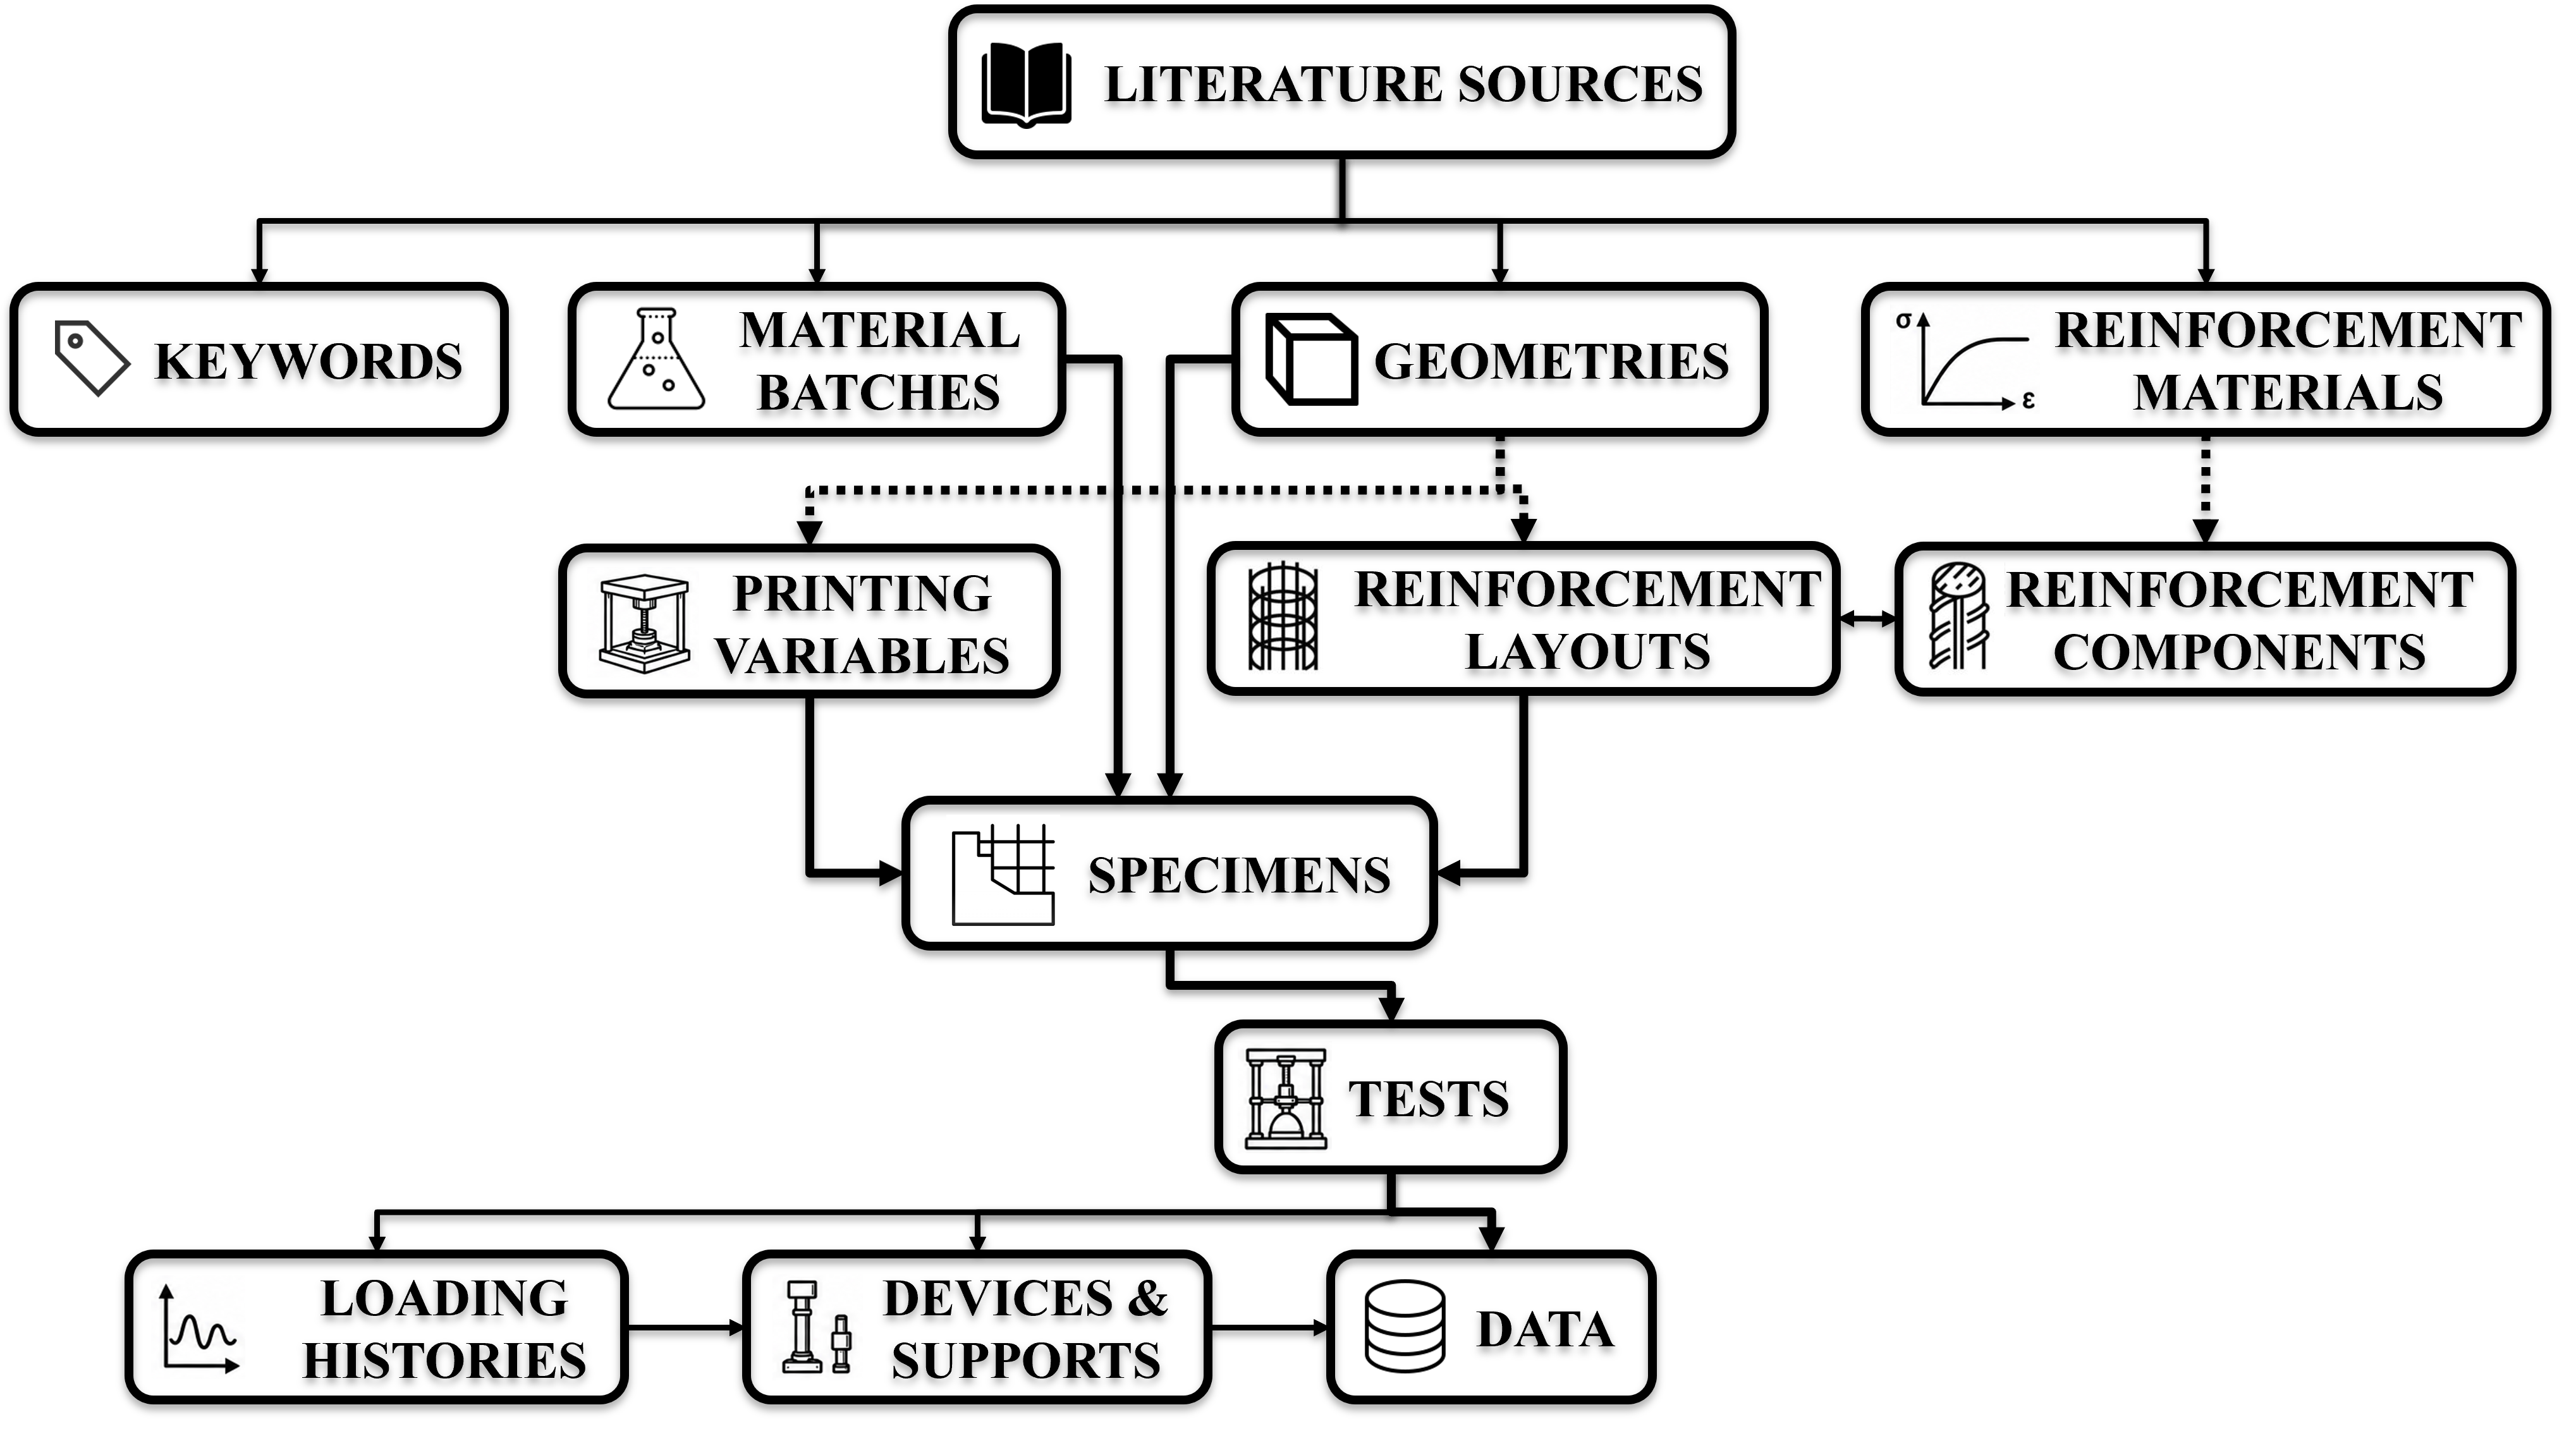
\includegraphics[width=0.9\linewidth]{./figs/database_hierarchy.png}
    \caption{Hierarchical organization of the database showing the relationships between literature sources, material batches, geometries, reinforcement materials, reinforcement components, reinforcement layouts, specimens, tests, devices and supports, loading histories, and experimental data entries.}
    \label{fig:database_hierarchy}
\end{figure}



\section{Database Hierarchy }
The database is organized according to a hierarchical structure designed to preserve the logical relationships between literature sources, material systems, specimen definitions, experimental tests, and associated datasets (Fig.~\ref{fig:database_hierarchy}). At the highest level, each literature source represents a publication, report, thesis, dataset, or experimental campaign from which the data originate. Literature sources are linked to keywords that facilitate indexing, search, and categorization, as well as to reusable definitions of material batches, geometries, reinforcement systems, printing variables, specimens, tests, and associated datasets.

Material batches describe the specific concrete mixtures or material systems investigated within a source. Geometries define reusable specimen geometrical configurations through standardized parametrizations provided in the geometry parametrization library. Printing variables provide reusable definitions relevant to additively manufactured specimens.

The reinforcement hierarchy is organized through three distinct but interconnected entities: reinforcement materials, reinforcement components, and reinforcement layouts. Reinforcement materials define reusable material properties associated with reinforcing systems. Reinforcement components represent individual reinforcement entities, such as longitudinal bar layers, stirrup sets, tie systems, or externally bonded reinforcement elements, and combine reinforcement geometry with the associated reinforcement material definition. Reinforcement layouts and components are associated with a specific geometry. Multiple reinforcement components are then assembled into reusable reinforcement layouts representing complete reinforcement configurations for specimens.

A specimen represents the combination of a material batch, geometry, reinforcement layout (if relevant), and optional printing variables (if relevant) associated with a physical specimen or specimen family.

Specimens are connected to individual tests that contain detailed information about the experimental procedures, environmental conditions, loading configurations, and observed physical mechanisms. Each test serves as the central entity to which additional components are attached, including devices and supports, loading histories, and the collected experimental data. Devices and supports may represent actuators, sensors, fixtures, supports, instrumentation systems, or measurement devices associated with the test setup. Loading histories define loading protocols or time histories associated with a test and, when relevant, with a specific device.

Experimental observations are organized through the data entity, which may include scalar quantities, curves, tables, images, videos, and multidimensional datasets together with their associated provenance and metadata. Data entries may optionally be linked to specific devices and supports when the measurements originate from a particular instrumentation component.


\section{Parametrization Schemes}

A major challenge in building a large-scale experimental database for concrete materials and structures is the enormous variability in specimen configurations, reinforcement layouts, boundary conditions, and testing procedures reported in the literature. Experimental programs are often described using highly heterogeneous terminology, inconsistent geometric definitions, incomplete drawings, or source-specific conventions that are difficult to interpret computationally. While this level of flexibility may be acceptable for traditional human interpretation of journal articles and reports, it creates severe limitations for machine readability and automated data extraction.

To address these challenges, the database adopts \textbf{standardized parametrization schemes} for 
\begin{enumerate}
    \item specimen geometries
    \item test setups
    \item reinforcement layouts
    \item devices, and supports configurations
\end{enumerate}

These parametrization schemes define a limited but extensible set of canonical representations capable of describing the vast majority of experimental configurations encountered in concrete and reinforced concrete mechanics research. The parametrizations are organized through dedicated geometry, test, reinforcement, devices, and supports libraries, described later in this documentation, that define standardized parameter names, coordinate conventions, and required descriptors.

\vspace{5mm}
The adoption of parametrized representations provides several important advantages.

\begin{enumerate}

\item \textbf{Machine readability and interoperability.} Standardized parametrizations transform heterogeneous experimental descriptions into structured machine-readable data. This enables automated parsing, validation, indexing, and integration across datasets originating from different laboratories, countries, and historical periods.

\item \textbf{Consistency across datasets.} Canonical parameter names and coordinate conventions reduce ambiguity and minimize inconsistent interpretations of geometry dimensions, reinforcement locations, support conditions, and loading configurations.

\item \textbf{Efficient storage and reduced redundancy.} Parametric descriptions require only a compact set of defining variables instead of large unstructured textual descriptions or multiple redundant drawings. The same parametrized geometry can also be reused across multiple tests.

\item \textbf{Automated generation of computational models.} Parametrized representations facilitate automatic generation of computational models . This capability is particularly important for future automated calibration, validation, and benchmarking workflows.

\item \textbf{Support for machine learning applications.} Machine learning models require consistent numerical descriptors rather than free-form textual descriptions. Parametrized geometries and reinforcement schemes provide structured low-dimensional feature representations that can be directly used for classification, clustering, regression, surrogate modeling, and uncertainty quantification.

\item \textbf{Scalability and future extensibility.} The parametrization libraries are designed to evolve over time. New geometry types, reinforcement configurations, and test setups can be added while preserving compatibility with existing datasets and workflows.

\item \textbf{Improved traceability and reproducibility.} Standardized parametrizations make it easier to reproduce experiments computationally and verify the consistency of reported dimensions, reinforcement layouts, and loading configurations.

\end{enumerate}

The parametrization schemes adopted in the current version of the database are designed to balance simplicity, extensibility, and practical usability. The objective is not to reproduce every possible geometric detail found in experimental programs, but rather to capture the dominant features required for computational modeling, data analytics, and systematic comparison across datasets. When experimental configurations cannot be adequately represented by the current libraries, contributors are encouraged to propose extensions and additional parametrization types as part of the ongoing evolution of the database framework.

\vspace{5mm}
\noindent
\fbox{%
  \parbox{\linewidth}{%
    \textbf{The absence of an existing parametrization scheme for a particular geometry, reinforcement configuration,  test setup, or device/support configuration is not a reason for exclusion from the database. In such cases, contributors should provide the most complete description possible using available metadata, drawings, images, parameter files, and notes, while also proposing potential extensions to the corresponding parametrization libraries.}
  }%
}



\section{Manual Data Submission}

Each submission must contain a single dataset only, which will be automatically appended to the overall database after validation and processing. Contributors should submit one dataset at a time to simplify quality control, provenance tracking, and integration into the centralized repository. All identifiers must follow the prescribed naming convention and begin with the numerical sequence \texttt{0001} for each new submission category, for example \texttt{SRC0001}, \texttt{BAT0001}, and \texttt{TST0001}. Contributors are expected to populate all relevant cells in the spreadsheet template as completely and accurately as possible.

The submitted dataset must follow the required folder hierarchy and include all relevant supporting files associated with the experimental program. The top-level directory must be named using the source identifier and should contain the completed spreadsheet template together with an optional Python script or Jupyter Notebook capable of plotting and visualizing all experimental curves included in the dataset. The general folder structure is illustrated below:

\begin{verbatim}
SRC0001/
    SRC0001.xlsx
    SRC0001.ipynb
    BAT0001/
        TST0001/
        TST0002/
        .../
    BAT0002/
        TST0003/
        .../
\end{verbatim}

Within each source directory, the spreadsheet stores the metadata and structured information associated with the experimental campaign, while the batch and test subdirectories contain all corresponding files such as CSV tables, loading histories, images, videos, geometry descriptions, measurement data, and other relevant artifacts. Each material batch is represented by a dedicated folder, and each experimental test associated with that batch is stored in its own test folder. Test numbering must remain progressive across all batches belonging to the same source.

Only data and files that can be legally redistributed should be included in the submission. Contributors must not upload copyrighted articles, scanned book chapters, or any other copyrighted material for which redistribution rights are unavailable. The submission should contain only the curated data, associated metadata, and supporting files necessary for interpretation and reuse of the experimental results.

After preparing the dataset and verifying the folder structure, contributors should compress the entire submission into a single ZIP archive using the following naming convention:

\begin{verbatim}
lastname_year_month_day_n.zip
\end{verbatim}

For example:

\begin{verbatim}
cusatis_2026_4-18_1.zip
cusatis_2026_4-18_2.zip
...
\end{verbatim}

The final ZIP archive should then be uploaded through the designated submission portal ({\emph{under development}}). Additional information regarding the upload procedure and repository access will be provided soon.

During ingestion into the centralized database, all local identifiers will be automatically mapped to globally unique database identifiers.

\section{AI-Assisted Data Submission}
{\emph{under development}}

\section{Use of AI Tools in Documentation and Schema Development}
This documentation was prepared with the assistance of artificial intelligence (AI) tools used to support drafting, editing, formatting, organizational tasks, controlled vocabulary definition suggestions, and generation of machine-readable JSON schema and library files. AI-assisted tools also contributed to consistency checking. All scientific, technical, and methodological content, including database architecture, parametrization schemes, controlled vocabularies, validation logic, and JSON definitions, was reviewed, validated, and curated by members of the Grand Challenge Working Group.

Given the scale, evolving nature, and technical complexity of the effort, the documentation and associated schema definitions may still contain inconsistencies, ambiguities, omissions, or unintended errors. Contributors and users are encouraged to report issues, suggest improvements, and propose extensions as part of the ongoing community-driven development of the database framework.


\section{Naming Conventions}

The following table summarizes the standardized identifier conventions adopted throughout the database to uniquely define the primary entities, metadata components, parametrization objects, and experimental data entries used in the submission workflow and database architecture.

\begin{longtable}{p{0.28\textwidth}p{0.13\textwidth}p{0.51\textwidth}}
\toprule
\textbf{Entity} & \textbf{ID Format} & \textbf{Meaning} \\
\midrule
Source & SRC0001 & One publication, report, thesis, dataset, or experimental campaign source \\
Material batches & BAT0001 & One material batch, mixture, or material system definition \\
Geometries & GEO0001 & One specimen geometry definition as defined in the geometry parametrization library \\
Printing variables & PRI0001 & One set of printing variables associated with an additively manufactured specimen \\
Reinforcement materials & RMT0001 & One reusable set of material properties associated with reinforcement systems \\
Reinforcement components & REF0001 & One reinforcement component, such as a reinforcement layer, stirrup set, or external reinforcement component, defined through the reinforcement parametrization library and associated with a reinforcement material \\
Reinforcement layouts & RFL0001 & One reinforcement layout combining multiple reinforcement components \\
Specimens & SPC0001 & One specimen definition combining material batch, geometry, reinforcement layout (if relevant), and printing variables (if relevant) \\
Tests & TST0001 & One experimental test or environmental exposure condition \\
Devices \& Supports & DEV0001 & One support, actuator, sensor, instrumentation component, or measurement device \\
Loading histories & LDG0001 & One loading protocol or loading history associated with a test \\
Data & DAT0001 & One scalar quantity, curve, table, image, video, or multidimensional dataset entry \\
\bottomrule
\end{longtable}

File names should be descriptive, machine readable, and should not contain spaces or special characters other than underscores, hyphens, and periods. Recommended separators are underscores. File names should also include the relevant entity identifier whenever possible to simplify traceability and automated parsing.

\vspace{5mm}
Examples include:

\begin{verbatim}
TST0001_load_displacement.csv
TST0001_temperature_history.csv
TST0001_test_setup.png
GEO0001_geometry_parameters.csv
REF0001_stress_strain_curve.csv
BAT0001_mixing_protocol.txt
DAT0001_crack_pattern_image.png
\end{verbatim}

Contributors should avoid ambiguous file names such as:

\begin{verbatim}
data.csv
image1.png
testfinal.csv
\end{verbatim}

Whenever possible, file names should reflect the physical meaning of the data, the associated entity, and the quantity being reported.
\section{Coordinate Systems}
All spatial information is defined using a right-handed Cartesian coordinate system with coordinates $x$, $y$, and $z$, where the origin and axis orientations are specified according to the reference configurations provided in the specimen geometry library. 

\section{Units Policy}
All numerical values must include associated units, either directly in the spreadsheet or in the second row of the corresponding CSV file. Certain spreadsheet entries require predefined units, which are explicitly indicated in the column header. For example, the cell with header \texttt{cement\_content\_kg\_m3} in the batch description sheet requires the cement content to be reported in units of kg/m$^3$. Contributors should strictly follow the prescribed units whenever they are specified in the column names to ensure consistency and compatibility across the database.


\begin{longtable}{p{0.30\textwidth}p{0.25\textwidth}p{0.35\textwidth}}
\toprule
\textbf{Quantity} & \textbf{Preferred Unit} & \textbf{Notes} \\
\midrule
Length & mm & Geometry, device locations, crack openings, displacements \\
Force & N or kN & Use consistently within each file \\
Stress & MPa & Preferred for concrete and reinforcement strength \\
Strain & dimensionless & Use decimal strain, not percent, unless explicitly stated \\
Density & kg/m$^3$ & Material constituents \\
Temperature & $^\circ$C & Environmental and thermal histories \\
Relative humidity & \% & Environmental histories \\
Time & s, min, h, or day & State explicitly \\
Mass content & kg/m$^3$ & Mix design quantities \\
Volume fraction & dimensionless or \% & State explicitly \\
... & ... & ... \\
\bottomrule
\end{longtable}

%============================================================
\section{File Standards}
%============================================================

\subsection{Curve CSV Formatting}

Curve CSV files must include two header rows followed by numerical values. The first row contains variable names. The second row contains units.

\begin{verbatim}
displacement,load
mm,kN
0.000,0.000
0.010,1.250
0.020,2.410
\end{verbatim}

For multiple curves, create separate files.

\subsection{Table CSV Formatting}

Table CSV files must include two header rows. The first row contains column names. The second row contains units. Leave the unit cell blank for unitless or string data.

\begin{verbatim}
specimen,compressive_strength,elastic_modulus
,MPa,MPa
A1,42.1,31000
A2,41.7,30500
\end{verbatim}

\subsection{Specimen Geometry Parametsrs CSV Formatting}

Geometry CSV files must contain three rows:

\begin{enumerate}
    \item parameter names;
    \item parameter units;
    \item parameter values.
\end{enumerate}

Example for a notched beam:

\begin{verbatim}
length,depth,thickness,notch_depth,notch_width,notch_tip_radius
mm,mm,mm,mm,mm,mm
500,100,100,30,3,1.5
\end{verbatim}

\subsection{HDF5 Recommendations}

For large field datasets, multidimensional arrays, time-dependent image stacks, or voxel data, CSV is not recommended. HDF5 should be used when data are large and/or multidimensional, for example DIC displacement and strain fields, 3D tomography data, voxelated microstructures. time-dependent temperature or moisture fields.

\subsection{JSON File Standards}

JSON files will be used throughout the database to define machine-readable vocabularies, parametrization libraries, validation schemas, metadata structures, and future API interfaces.

In general, CSV files are intended for tabular numerical data such as curves, loading histories, tables, and simple parameter lists, whereas JSON files are intended for structured metadata, parametrization definitions, hierarchical relationships, validation schemas, and
machine-readable database definitions.

JSON files should follow the following conventions:

\begin{itemize}
    \item UTF-8 encoding;
    \item four-space indentation;
    \item lowercase underscore-separated field names;
    \item explicit units whenever numerical quantities are included;
    \item standardized database identifiers such as
    \texttt{source\_id}, \texttt{batch\_id},
    \texttt{specimen\_id}, \texttt{geometry\_id},
    and \texttt{test\_id}.
\end{itemize}

JSON files should conform to the associated
JSON Schema validation ({\emph{under development}}) definitions that will be distributed with the database.


\section{Controlled Vocabularies}
The spreadsheet uses controlled vocabularies (Part \ref{Part:Vocab}), primarily through dropdown lists provided in the \texttt{Vocab} tab and through accompanying machine-readable JSON vocabulary definition files ({\emph{under development}}).

\vspace{5mm}
\noindent
\fbox{%
  \parbox{\linewidth}{%
    \textbf{Whenever possible, contributors should select existing entries from the predefined vocabularies rather than introducing custom terminology or abbreviations. If an appropriate vocabulary entry does not exist, contributors are encouraged to propose new entries together with concise definitions and, when relevant, associated units or parameter descriptions. The vocabulary system is extensible and will evolve continuously as the database expands.}
  }%
}
\vspace{5mm}

Vocabulary entries should generally follow lowercase underscore-separated naming conventions. 

\vspace{5mm}
For example:

\begin{verbatim}
three_point_bending
chloride_diffusion
carbon_fiber_reinforced_polymer
reversed_cyclic_loading
\end{verbatim}

The recommended format for observed mechanisms is:

\begin{verbatim}
category | mechanism_name
\end{verbatim}

This two-level structure separates the broad physical category from the specific observed mechanism, facilitating semantic grouping and database queries.

\vspace{5 mm}
Examples:

\begin{verbatim}
strength | unconfined_compressive_failure
fracture | fracture_propagation
transport | chloride_diffusion
fresh | workability
thermal | adiabatic_temperature_rise
durability | alkali_silica_reaction
bond | reinforcement_pullout
\end{verbatim}

Multiple mechanisms may be entered in one cell separated by commas. For example:

\begin{verbatim}
fracture | crack_localization, strength | tensile_failure
\end{verbatim}

\section{Required vs Optional Tabs and Fields}

The data collection template contains both required and optional tabs and fields. Required tabs and fields must be completed for the dataset to be accepted into the database. Optional fields should still be completed whenever the corresponding information is available. A field may be classified as optional because the information is not always reported in historical publications, reports, or experimental records. However, contributors are strongly encouraged to provide all available information to maximize dataset completeness, traceability, and long-term usability.

The table below summarizes the tabs included in the data collection template together with their requirement status and the conditions under which each tab must be completed.

\begin{longtable}{p{0.32\textwidth}p{0.58\textwidth}}
\hline
\textbf{Tab Name} & \textbf{Requirement Status and Conditions} \\
\hline
\endfirsthead

\hline
\textbf{Tab Name} & \textbf{Requirement Status} \\
\hline
\endhead

\texttt{literature\_sources} &
\textcolor{red}{Required} for all dataset submissions.  \\

\texttt{keywords} &
\textcolor{red}{Required} for all dataset submissions.  \\

\texttt{material\_batches} &
\textcolor{red}{Required} for all dataset submissions. \\

\texttt{geometries} &
\textcolor{red}{Required} for all dataset submissions. \\

\texttt{specimens} &
\textcolor{red}{Required} for all dataset submissions. \\

\texttt{tests} &
\textcolor{red}{Required} for all dataset submissions. \\

\texttt{data} &
\textcolor{red}{Required} for all dataset submissions. \\

\texttt{reinforcement\_materials} &
\textcolor{orange}{Conditionally required} if reinforcement materials are present in the specimens. \\

\texttt{reinforcement\_layouts} &
\textcolor{orange}{Conditionally required} if reinforcement materials are present in the specimens. \\

\texttt{reinforcement\_components} &
\textcolor{orange}{Conditionally required} if reinforcement materials are present in the specimens. \\

\texttt{printing\_variables} &
\textcolor{orange}{Conditionally required} if the specimen is additively manufactured. \\

\texttt{devices\_and\_supports} &
\textcolor{green}{Optional} but recommended if instrumentation devices, supports, fixtures, actuators, sensors, or boundary-condition components are available. \\

\texttt{loading\_histories} &
\textcolor{green}{Optional} but recommended if loading protocols, cyclic histories, displacement histories, force histories, or time-dependent loading information are reported. \\

\hline
\end{longtable}

Fields marked as required within each tab are used during automated dataset validation procedures to verify completeness, consistency, identifier relationships, schema compliance, and conformity with the adopted controlled vocabularies. Datasets missing required tabs or required fields may be rejected or flagged for manual review prior to ingestion into the centralized database.

Examples of optional but highly encouraged information include DOI identifiers, detailed device metadata, environmental conditions, extraction dates, notes, supplementary geometry files, and supplementary loading or instrumentation descriptions. Providing this information substantially improves dataset traceability, interoperability, reproducibility, and future reuse for computational modeling, benchmark studies, and AI-assisted data analysis workflows.



\newpage

%============================================================
\chapter{Step-by-Step Manual Submission Workflow - Deprecated}
%============================================================

\section{Create Source Folder}

Create one folder for the dataset. The folder must be named using the source identifier:

\begin{verbatim}
SRC0001
\end{verbatim}

Only one dataset should be submitted at a time. Copy the template spreadsheet into the source folder and rename it:

\begin{verbatim}
SRC0001.xlsx
\end{verbatim}

%Populate the workbook tabs in the order described in this document. Begin with Literature\_sources and Keywords, then continue with Material\_batches, Geometry, Tests, Reinforcement, Printing\_variables, Devices\_and\_Supports, Loading\_Histories, and Data.

\section{Create Batch Folders}

For each material batch, create a folder inside the source folder:

\begin{verbatim}
SRC0001/BAT0001
SRC0001/BAT0002
\end{verbatim}

Each batch folder must correspond to one row in the \texttt{material\_batches} tab.

\section{Create Test Folders}

For each test, create a folder inside the corresponding batch folder:

\begin{verbatim}
SRC0001/BAT0001/TST0001
SRC0001/BAT0001/TST0002
SRC0001/BAT0002/TST0003
\end{verbatim}

Use progressive numbering across batches. Do not restart test numbering for each batch.

\section{Populate the \texttt{literature\_sources} Tab}

The \texttt{literature\_sources} table records bibliographic and identifying information for the source document, dataset, report, thesis, or experimental campaign from which the submitted data were extracted. The \texttt{source\_id} is referenced throughout the database hierarchy and serves as the top-level identifier linking all associated batches, specimens, tests, loading histories, devices, and experimental data. In manual submission, use \texttt{SRC0001} consistently. During ingestion into the centralized database, local identifiers will be automatically mapped to globally unique database identifiers while preserving the original submitted identifiers for traceability.

%\small
\setlength{\tabcolsep}{4pt}

\begin{longtable}{p{0.24\textwidth}p{0.06\textwidth}p{0.12\textwidth}p{0.5\textwidth}}
\hline
\textbf{Field} & \textbf{Req.} & \textbf{Type} & \textbf{Description} \\
\hline
\endfirsthead

\hline
\textbf{Field} & \textbf{Req.} & \textbf{Type} & \textbf{Description} \\
\hline
\endhead

\hline
\endfoot

\texttt{source\_id} & \textcolor{red}{Yes} & String & Identifier of the source document or dataset. Use \texttt{SRC0001} for manual submission. \\

\texttt{source\_type} & No & Vocab & Type of source. Examples include journal article, report, thesis, dataset, conference paper, or technical report. \\

\texttt{peer\_reviewed} & No & yes/no & Indicates whether the source was peer reviewed. \\

\texttt{title} & \textcolor{red}{Yes} & Text & Full title of the source. \\

\texttt{authors} & \textcolor{red}{Yes} & Text & Author list as reported in the source. Use comma separation. \\

\texttt{year} & No & Integer & Publication or release year. \\

\texttt{journal\_or\_publisher} & No & Text & Journal name, publisher, report agency, hosting institution, or conference proceedings. \\

\texttt{volume} & No & Text & Volume number if available. \\

\texttt{issue} & No & Text & Issue number if available. \\

\texttt{pages} & No & Text & Page range or article number. \\

\texttt{doi} & No & Text & Digital object identifier. Optional only because older sources may not have one. \\

\texttt{url} & No & Text & URL to the source or dataset record. \\

\texttt{institution} & No & Text & Institution associated with a report, thesis, dataset, or experimental campaign. \\

\texttt{notes} & No & Text & Any information useful to identify the source, especially when DOI or URL information is unavailable. \\

\end{longtable}
%\normalsize

\section{Populate the \texttt{keywords} Tab}

The \texttt{keywords} table records a \textbf{minimum of five keywords} describing the dataset. Keywords are associated with the \texttt{source\_id} and describe the dataset as a whole rather than one specific specimen or test.

\setlength{\tabcolsep}{4pt}

\begin{longtable}{p{0.24\textwidth}p{0.06\textwidth}p{0.12\textwidth}p{0.5\textwidth}}
\hline
\textbf{Field} & \textbf{Req.} & \textbf{Type} & \textbf{Description} \\
\hline
\endfirsthead

\hline
\textbf{Field} & \textbf{Req.} & \textbf{Type} & \textbf{Description} \\
\hline
\endhead

\hline
\endfoot

\texttt{source\_id} & \textcolor{red}{Yes} & String & Identifier of the source associated with the keyword. Use \texttt{SRC0001} for manual submission. \\

\texttt{keyword} & \textcolor{red}{Yes} & Text & Searchable keyword describing material systems, tests, mechanisms, methods, environmental conditions, or data types associated with the dataset. \\

\end{longtable}

\section{Populate the \texttt{material\_batches} Tab}

The \texttt{material\_batches} table describes each concrete mixture, batch, or material system reported in the source. One row corresponds to one distinct material formulation. Each batch references one source through \texttt{source\_id}. The material batch definition is independent of specimen geometry and testing configuration, allowing the same material system to be reused across multiple specimens and tests.

The table supports conventional cement paste, mortar, concrete, fiber-reinforced concrete, cementitious composites, cementitious mixture for additive manufacturing, and other cementitious materials relevant to the database scope. When available, a text file describing the mixing protocol should be included in the corresponding batch folder.

\small
\begin{longtable}{p{0.38\textwidth}p{0.04\textwidth}p{0.08\textwidth}p{0.06\textwidth}p{0.34\textwidth}}

\textbf{Field} & \textbf{Req.} & \textbf{Type} & \textbf{Units} & \textbf{Description} \\
\hline
\endfirsthead

\textbf{Field} & \textbf{Req.} & \textbf{Type} & \textbf{Units} & \textbf{Description} \\
\hline
\endhead

\texttt{batch\_id} & \textcolor{red}{Yes} & String & none & Unique identifier for the material batch. Must correspond to the batch folder name. \\

\texttt{source\_id} & \textcolor{red}{Yes} & String & none & Source identifier. \\

\texttt{mixing\_protocol\_file\_name} & No & String & none & Text file describing the mixing, batching, curing, or specimen preparation protocol. \\

\texttt{batch\_label} & No & Text & none & Label used in the original source. \\

\texttt{material\_class} & \textcolor{red}{Yes} & Vocab & none & General material class. \\

\texttt{cement\_type} & No & Vocab & none & Cement classification, designation, or product description. \\

\texttt{printable} & No & yes/no & none & Indicates whether the material is intended for additive manufacturing or extrusion-based fabrication. \\

\texttt{self\_consolidating} & No & yes/no & none & Indicates whether the material is self consolidating. \\

\texttt{cement\_content\_kg\_m3} & \textcolor{red}{Yes} & Number & kg/m$^3$ & Cement mass per unit concrete volume. \\

\texttt{water\_binder\_ratio} & \textcolor{red}{Yes} & Number & - & Ratio of water mass to total binder mass. \\

\texttt{silica\_fume\_content\_kg\_m3} & No & Number & kg/m$^3$ & Silica fume content. \\

\texttt{fly\_ash\_content\_kg\_m3} & No & Number & kg/m$^3$ & Fly ash content. \\

\texttt{fly\_ash\_class} & No & Vocab & - & Fly ash class if reported. \\

\texttt{slag\_content\_kg\_m3} & No & Number & kg/m$^3$ & Slag cement content. \\

\texttt{fine\_aggregate\_content\_kg\_m3} & No & Number & kg/m$^3$ & Fine aggregate mass per unit concrete volume. \\

\texttt{fine\_aggregate\_dry\_density\_kg\_m3} & No & Number & kg/m$^3$ & Dry density of fine aggregate. \\

\texttt{coarse\_aggregate\_content\_kg\_m3} & No & Number & kg/m$^3$ & Coarse aggregate mass per unit concrete volume. \\

\texttt{coarse\_aggregate\_dry\_density\_kg\_m3} & No & Number & kg/m$^3$ & Dry density of coarse aggregate. \\

\texttt{max\_aggregate\_size\_mm} & No & Number & mm & Maximum aggregate size. \\

\texttt{aggregate\_type} & No & Vocab & none & Aggregate mineralogy, lithology, or aggregate description. \\

\texttt{superplasticizer\_type} & No & Text & none & Superplasticizer type or commercial product designation. \\

\texttt{superplasticizer\_content\_kg\_m3} & No & Number & kg/m$^3$ & Superplasticizer dosage by mass. \\

\texttt{water\_reducer\_type} & No & Text & none & Water reducer type or commercial product designation. \\

\texttt{water\_reducer\_content\_ml\_m3} & No & Number & ml/m$^3$ & Water reducer dosage by volume. \\

\texttt{air\_entrainment\_type} & No & Text & none & Air entraining admixture type or product designation. \\

\texttt{air\_entrainment\_content\_ml\_m3} & No & Number & ml/m$^3$ & Air entrainment dosage. \\

\texttt{rheology\_modifier\_type} & No & Text & none & Rheology modifying admixture type or product designation. \\

\texttt{rheology\_modifier\_content\_kg\_m3} & No & Number & kg/m$^3$ & Rheology modifier dosage. \\

\texttt{hydration\_accelerator\_type} & No & Text & none & Hydration accelerator type or product designation. \\

\texttt{hydration\_accelerator\_content\_ml\_m3} & No & Number & ml/m$^3$ & Hydration accelerator dosage. \\

\texttt{fiber\_type} & No & Vocab & none & Fiber material and fiber form. \\

\texttt{fiber\_product\_name} & No & Text & none & Commercial fiber product name if available. \\

\texttt{fiber\_volume\_fraction} & No & Number & none or \% & Fiber volume fraction. State whether decimal or percent notation is used. \\

\texttt{fiber\_length\_mm} & No & Number & mm & Fiber length. \\

\texttt{fiber\_diameter\_mm} & No & Number & mm & Fiber diameter. \\

\texttt{air\_content\_percent\_volume\_concrete} & No & Number & \% & Air content by concrete volume. \\

\texttt{date\_of\_pouring\_yyyy-mm-dd} & No & Date & date & Casting date in ISO format. \\

\texttt{notes} & No & Text & none & Additional information about the mixture, batching procedure, curing protocol, constituent materials, or specimen preparation. \\

\hline

\end{longtable}
\normalsize

\section{Populate the \texttt{reinforcement\_materials} Tab}

The \texttt{reinforcement\_materials} tab defines reusable reinforcement material property records that can be referenced by multiple reinforcement components throughout the database. Each entry is uniquely identified by a \texttt{reinforcement\_material\_id}. The tab depends hierarchically on the \texttt{literature\_sources} tab and serves as a parent entity for the \texttt{reinforcement\_components} tab. 


\begin{longtable}{p{0.31\textwidth}p{0.05\textwidth}p{0.08\textwidth}p{0.10\textwidth}p{0.34\textwidth}}

\hline
\textbf{Field} &
\textbf{Req.} &
\textbf{Type} &
\textbf{Units} &
\textbf{Description} \\
\hline
\endfirsthead

\hline
\textbf{Field} &
\textbf{Req.} &
\textbf{Type} &
\textbf{Units} &
\textbf{Description} \\
\hline
\endhead

\texttt{reinforcement\_material\_id} &
\textcolor{red}{Yes} &
String &
none &
Unique reinforcement identifier. \\

\texttt{source\_id} &
\textcolor{red}{Yes} &
String &
none &
Source identifier. \\

\texttt{reinforcement\_material\_type} &
No &
Vocab &
none &
Reinforcement material type. \\

\texttt{stress\_strain\_curve\_file} &
No &
File name &
none &
CSV file containing the constitutive response of the reinforcement material. \\

\texttt{elastic\_modulus\_mpa} &
No &
Number &
MPa &
Elastic modulus of reinforcement material. \\

\texttt{yield\_strength\_mpa} &
No &
Number &
MPa &
Yield strength of reinforcement material. \\

\texttt{rupture\_strength\_mpa} &
No &
Number &
MPa &
Ultimate or rupture strength of reinforcement material. \\

\texttt{rupture\_strain} &
No &
Number &
none &
Rupture strain of reinforcement material. \\

\texttt{notes} &
No &
Text &
none &
Additional reinforcement information. \\

\hline

\end{longtable}

The \texttt{stress\_strain\_curve\_file} field identifies a file containing the constitutive response of the reinforcement material. The file includes stress-strain data describing the mechanical behavior of the reinforcement material under uniaxial loading. The data may represent experimental measurements, manufacturer-provided constitutive curves, or idealized constitutive relationships used in numerical simulations.

The file must contain two header rows followed by as many rows as needed to define the stress-strain curve:

\begin{enumerate}
    \item variable names separated by commas;
    \item variable units separated by commas;
    \item stress-strain data rows separated by commas.
\end{enumerate}

General format:

\begin{verbatim}
strain,stress
-,MPa
e0,s0
e1,s1
...
en,sn
\end{verbatim}

Example:

\begin{verbatim}
strain,stress
-,MPa
0.0000,0
0.0010,200
0.0020,420
0.0500,550
...
\end{verbatim}




\section{Populate the \texttt{geometries} Tab}

The \texttt{geometries} tab stores information describing the specimen geometry independently of the material batch, reinforcement configuration, specimen definition, and experimental test. Its main purpose is to define reusable geometric representations of specimens using standardized parametrizations provided in the geometry parametrization library. Each geometry entry defines the physical shape and dimensions of a specimen configuration that may later be associated with one or more specimen definitions and experimental tests.

Only geometries currently defined in the geometry parametrization library are presently supported. When a geometry type cannot be adequately represented using the existing library, contributors are encouraged to propose extensions together with the associated parameter definitions and coordinate conventions.


\begin{longtable}{>{\raggedright\arraybackslash}p{0.31\textwidth}
                  >{\raggedright\arraybackslash}p{0.05\textwidth}
                  >{\raggedright\arraybackslash}p{0.10\textwidth}
                  >{\raggedright\arraybackslash}p{0.07\textwidth}
                  >{\raggedright\arraybackslash}p{0.36\textwidth}}
\hline
\textbf{Field} &
\textbf{Req.} &
\textbf{Type} &
\textbf{Units} &
\textbf{Description} \\
\hline
\endfirsthead

\hline
\textbf{Field} &
\textbf{Req.} &
\textbf{Type} &
\textbf{Units} &
\textbf{Description} \\
\hline
\endhead

\texttt{geometry\_id} & \textcolor{red}{Yes} & String & none & Unique geometry identifier. \\

\texttt{source\_id} & \textcolor{red}{Yes} & String & none & Source identifier. \\

\texttt{specimen\_geometry\_type} & \textcolor{red}{Yes} & Vocab & none & Geometry type from the geometry parametrization library. \\

\texttt{geometry\_file\_name} & \textcolor{red}{Yes} & File name & none & CSV or JSON file containing the geometry parameter names, units, and parameter values according to the geometry parametrization library. \\

\texttt{notes} &
No &
Text &
none &
Additional geometry information. \\


\hline
\end{longtable}

For each geometry row, create a geometry CSV or JSON file and place it in the corresponding source folder associated with the dataset.


The geometry parameters, parameter names, coordinate conventions, and required dimensions are defined in the geometry parametrization library. The current library includes standardized parametrizations for prisms, cubes, cylinders, beams, notched beams, panels, walls, plates, L-shaped specimens, dog-bone specimens, and other common experimental configurations.


The CSV file must contain exactly three rows: (1) parameter names separated by commas; (2) parameter units separated by commas; (3) parameter values separated by commas.

\vspace{5mm}
CSV example for \texttt{notched\_prism}:


\begin{verbatim}
prism_length,prism_depth,prism_thickness,notch_offset,
notch_depth,notch_width,notch_tip_radius
mm,mm,mm,mm,mm,mm,mm
500.0,100.0,100.0,0.0,30.0,3.0,1.5
\end{verbatim}

The JSON file must conform to the specifications defined in \texttt{geometry\_schema.json}.

\vspace{5mm}
Example for \texttt{prism}

\begin{verbatim}
{
  "geometry_id": "GEO0001",
  "source_id": "SRC0001",
  "specimen_geometry_type": "prism",
  "coordinate_system": {
    "origin": "corner point shown in the prism geometry scheme",
    "x_axis": "longitudinal direction along the prism length",
    "y_axis": "transverse direction along the prism thickness",
    "z_axis": "vertical direction along the prism depth"
  },
  "parameters": {
    "length": {
      "value": 500.0,
      "unit": "mm"
    },
    "thickness": {
      "value": 100.0,
      "unit": "mm"
    },
    "depth": {
      "value": 100.0,
      "unit": "mm"
    }
  }
}
\end{verbatim}


Contributors should ensure that all geometric parameters are reported consistently with the coordinate system and parameter definitions specified in the geometry parametrization library. A drawing, CAD file, annotated figure, or image describing the specimen geometry may also be included in the dataset when available through the \texttt{geometry\_file\_name} field. This supplementary file does not replace the required parametric geometry definition.

\section{Populate the \texttt{printing\_variables} Tab}
{\emph{under development}}




\section{Populate the \texttt{reinforcement\_layouts} Tab}

The \texttt{reinforcement\_layouts} tab defines reinforcement configurations associated with specimen geometries but reusable for the definition of multiple specimens. Each entry in this tab represents a complete reinforcement layout composed of one or more reinforcement components subsequently defined in the \texttt{reinforcement\_components} tab. A single reinforcement layout may therefore be associated with multiple entries in the \texttt{reinforcement\_components} tab, each describing one constituent reinforcement component together with its associated reinforcement material properties.

The tab supports three principal reinforcement categories:

\begin{itemize}
\item longitudinal tensile and flexural reinforcement;
\item transverse reinforcement systems such as stirrups, ties, and confinement reinforcement;
\item externally bonded or externally attached reinforcement systems, including externally bonded FRP laminates, sheets, and mechanically attached strengthening systems.
\end{itemize}



\begin{longtable}{>{\raggedright\arraybackslash}p{0.31\textwidth}
                  >{\raggedright\arraybackslash}p{0.05\textwidth}
                  >{\raggedright\arraybackslash}p{0.10\textwidth}
                  >{\raggedright\arraybackslash}p{0.07\textwidth}
                  >{\raggedright\arraybackslash}p{0.36\textwidth}}
\hline
\textbf{Field} &
\textbf{Req.} &
\textbf{Type} &
\textbf{Units} &
\textbf{Description} \\
\hline
\endfirsthead

\hline
\textbf{Field} &
\textbf{Req.} &
\textbf{Type} &
\textbf{Units} &
\textbf{Description} \\
\hline
\endhead

\texttt{reinforcement\_layout\_id} & \textcolor{red}{Yes} & String & none & Unique specimen identifier. \\

\texttt{source\_id} & \textcolor{red}{Yes} & String & none & Source identifier. \\

\texttt{geometry\_id} & \textcolor{red}{Yes} & String & none & Geometry identifier referencing an entry in the \texttt{Geometry} tab. \\

\texttt{longitudinal\_reinforcement} & \textcolor{red}{Yes} & yes/no & none & Indicates presence of longitudinal reinforcement. \\

\texttt{transverse\_reinforcement} & \textcolor{red}{Yes} & yes/no & none & Indicates presence of transverse reinforcement such as stirrups or ties. \\

\texttt{external\_reinforcement} & \textcolor{red}{Yes} & yes/no & none & Indicates presence of externally bonded or externally attached reinforcement systems. \\

\texttt{reinforcement\_file\_name} &
No &
File name &
none &
Optional drawing, CAD file, schematic, annotated image, or supplementary reinforcement description file. \\

\texttt{notes} & No & Text & none & Additional information describing the reinforcement configuration, reinforcement arrangement, fabrication procedure, etcetera. \\

\hline
\end{longtable}







\section{Populate the \texttt{reinforcement\_components} Tab}



The \texttt{reinforcement\_components} tab defines reusable reinforcement components associated with reinforcement layouts. Each entry represents one reinforcement component, such as a rebar layer, stirrup set, or external reinforcement system, and is uniquely identified by a \texttt{reinforcement\_component\_id} using the format \texttt{REF0001}.

The tab depends hierarchically on the \texttt{literature\_sources}, \texttt{reinforcement\_materials}, and \texttt{reinforcement\_layouts} tabs. Each reinforcement component combines geometric and placement information with the corresponding reinforcement material properties referenced through the \texttt{reinforcement\_material\_id}. Multiple reinforcement components may be associated with the same reinforcement layout to define complete reinforcement configurations consistently with the coordinate system and parametrization of the associated specimen geometry.

For each reinforcement entry, all geometric parameters, coordinate definitions, and orientation conventions must follow the parametrizations defined in the reinforcement parametrization library. 


Populate cells A-G with general information about the reinforcement. Populate cells H-Q if the reinforcement consists of tensile reinforcement, stirrups, or ties. Populate cells R-AL if the reinforcement consists of external reinforcement systems such as FRP wraps, plates, sheets, or externally bonded laminates.

\begin{longtable}{p{0.31\textwidth}p{0.05\textwidth}p{0.08\textwidth}p{0.10\textwidth}p{0.34\textwidth}}

\hline
\textbf{Field} &
\textbf{Req.} &
\textbf{Type} &
\textbf{Units} &
\textbf{Description} \\
\hline
\endfirsthead

\hline
\textbf{Field} &
\textbf{Req.} &
\textbf{Type} &
\textbf{Units} &
\textbf{Description} \\
\hline
\endhead

\multicolumn{5}{l}{\textbf{General Reinforcement Information: Cells A-G}} \\
\hline

\texttt{reinforcement\_component\_id} &
\textcolor{red}{Yes} &
String &
none &
Unique reinforcement identifier. \\

\texttt{source\_id} &
\textcolor{red}{Yes} &
String &
none &
Source identifier. \\

\texttt{reinforcement\_material\_id} &
\textcolor{red}{Yes} &
String &
none &
Associated reinforcement material identifier. \\

\texttt{reinforcement\_layout\_id} &
\textcolor{red}{Yes} &
String &
none &
Associated reinforcement layout identifier. \\

\texttt{notes} &
No &
Text &
none &
Additional reinforcement information. \\

\texttt{reinforcement\_type} &
\textcolor{red}{Yes} &
Vocab &
none &
Reinforcement type from the controlled vocabulary. \\

\texttt{reinforcement\_orientation} &
\textcolor{red}{Yes} &
Vocab &
none &
Principal reinforcement orientation relative to the specimen coordinate system. \\


\hline
\multicolumn{5}{l}{\textbf{Tensile Reinforcement, Stirrups, and Ties: Cells H-Q}} \\
\hline


\texttt{number\_of\_reinf\_elements} &
No &
Integer &
none &
Number of reinforcement bars, stirrups, or ties represented by the entry. \\

\texttt{bar\_designation} &
No &
Vocab &
none &
Standard reinforcement bar designation if applicable. If included, it may pre-populate the nominal diameter and area fields. \\

\texttt{bar\_nominal\_diameter\_mm} &
No &
Number &
mm &
Nominal reinforcement diameter. It is prepopulated if a standard bar designation is selected. It requires input if ``other'' is selected in bar designation.\\

\texttt{bar\_nominal\_area\_mm2} &
No &
Number &
mm$^2$ &
Nominal reinforcement cross-sectional area. It is prepopulated if a standard bar designation is selected. It requires input if ``other'' is selected in bar designation.\\

\texttt{layer\_depth\_mm} &
No &
Number &
mm &
Depth of the reinforcement layer measured in the associated system of reference. Leave empty for stirrups and ties when not applicable. \\

\texttt{spacing\_mm} &
No &
Number &
mm &
Center-to-center spacing between reinforcement elements. For longitudinal reinforcement this represents spacing between adjacent bars in a layer. For stirrups and ties this represents longitudinal spacing. \\

\texttt{horizontal\_cover\_mm} &
No &
Number &
mm &
Horizontal concrete cover. \\

\texttt{vertical\_cover\_mm} &
No &
Number &
mm &
Vertical concrete cover. \\

\texttt{begin\_distance\_mm} &
No &
Number &
mm &
Distance from the specimen origin to the beginning of the reinforcement system. \\

\texttt{end\_distance\_mm} &
No &
Number &
mm &
Distance from the specimen origin to the end of the reinforcement system. \\

\hline
\multicolumn{5}{l}{\textbf{External Reinforcement Systems: Cells R-AL}} \\
\hline

\texttt{reinforcement\_centroid\_x\_mm} &
No &
Number &
mm &
x-coordinate of the external reinforcement centroid. \\

\texttt{reinforcement\_centroid\_y\_mm} &
No &
Number &
mm &
y-coordinate of the external reinforcement centroid. \\

\texttt{reinforcement\_centroid\_z\_mm} &
No &
Number &
mm &
z-coordinate of the external reinforcement centroid. \\

\texttt{reinforcement\_width\_mm} &
No &
Number &
mm &
Width of the external reinforcement system. \\

\texttt{reinforcement\_length\_mm} &
No &
Number &
mm &
Length of the external reinforcement system. \\

\texttt{reinforcement\_thickness\_mm} &
No &
Number &
mm &
Thickness of the external reinforcement system. \\

\texttt{reinforcement\_angle\_deg} &
No &
Number &
deg &
Orientation angle of the external reinforcement with respect to the structural member axis. \\

\texttt{adhesive\_type} &
No &
Vocab &
none &
Adhesive or bonding material type. \\

\texttt{adhesive\_thickness\_mm} &
No &
Number &
mm &
Thickness of the adhesive layer. \\

\texttt{adhesive\_modulus\_mpa} &
No &
Number &
MPa &
Elastic modulus of the adhesive material. \\

\texttt{adhesive\_strength\_mpa} &
No &
Number &
MPa &
Adhesive strength. \\

\texttt{adhesive\_failure\_strain} &
No &
Number &
none &
Adhesive failure strain. \\

\texttt{anchorage\_presence} &
No &
yes/no &
none &
Indicates whether anchorage systems are present. \\

\texttt{anchorage\_type} &
No &
Vocab &
none &
Type of anchorage system. \\

\texttt{anchorage\_size\_mm} &
No &
Number &
mm &
Characteristic anchorage size or diameter. \\

\texttt{anchorage\_location\_x\_mm} &
No &
Number &
mm &
x-coordinate of the anchorage location. \\

\texttt{anchorage\_location\_y\_mm} &
No &
Number &
mm &
y-coordinate of the anchorage location. \\

\texttt{anchorage\_location\_z\_mm} &
No &
Number &
mm &
z-coordinate of the anchorage location. \\

\texttt{anchorage\_modulus\_mpa} &
No &
Number &
MPa &
Elastic modulus of the anchorage material. \\

\texttt{anchorage\_strength\_mpa} &
No &
Number &
MPa &
Strength of the anchorage material. \\

\texttt{anchorage\_failure\_strain} &
No &
Number &
none &
Failure strain of the anchorage material. \\

\hline

\end{longtable}







\section{Populate the \texttt{specimens} Tab}

The \texttt{specimens} tab defines the physical specimens or specimen families used in the experimental program. Each entry is uniquely identified by a \texttt{specimen\_id} using the format \texttt{SPC0001} and combines the corresponding material batch, geometry definition, and reinforcement and printing variables (if relevants) into a single specimen definition.

The tab depends hierarchically on the \texttt{literature\_sources}, \texttt{material\_batches}, \texttt{geometries}, \texttt{printing\_variables}, and \texttt{reinforcement\_layouts} tabs. It serves as the parent entity for the \texttt{tests} tab, enabling multiple experimental tests to be associated with the same specimen definition.

\begin{longtable}{>{\raggedright\arraybackslash}p{0.31\textwidth}
                  >{\raggedright\arraybackslash}p{0.05\textwidth}
                  >{\raggedright\arraybackslash}p{0.10\textwidth}
                  >{\raggedright\arraybackslash}p{0.07\textwidth}
                  >{\raggedright\arraybackslash}p{0.36\textwidth}}
\hline
\textbf{Field} &
\textbf{Req.} &
\textbf{Type} &
\textbf{Units} &
\textbf{Description} \\
\hline
\endfirsthead

\hline
\textbf{Field} &
\textbf{Req.} &
\textbf{Type} &
\textbf{Units} &
\textbf{Description} \\
\hline
\endhead

\texttt{specimen\_id} & \textcolor{red}{Yes} & String & none & Unique specimen identifier. \\

\texttt{source\_id} & \textcolor{red}{Yes} & String & none & Source identifier. \\

\texttt{batch\_id} & \textcolor{red}{Yes} & String & none & Associated material batch identifier. \\

\texttt{geometry\_id} & \textcolor{red}{Yes} & String & none & Geometry identifier referencing an entry in the \texttt{Geometry} tab. \\

\texttt{reinforcement\_layout\_id} & \textcolor{red}{Yes} & String & none & Geometry identifier referencing an entry in the \texttt{Geometry} tab. \\

\texttt{printing\_variables\_id} & \textcolor{red}{Yes} & String & none & Geometry identifier referencing an entry in the \texttt{Geometry} tab. \\

\texttt{structural\_form} & No & Vocab & none &
Classification describing the overall structural configuration, load-carrying mechanism, or structural member category of the specimen. \\

\texttt{notes} & No & Text & none & Additional information describing not included elsewhere in the tab. \\

\hline
\end{longtable}



\section{Populate the \texttt{tests} Tab}

The \texttt{Tests} tab records information about each experimental test performed on a specimen or structural component. Its purpose is to provide a standardized description of the testing procedure, environmental conditions, loading configuration, and observed physical response associated with the experiment.

The tab includes information about the test type, specimen age at testing, curing history, thermal and hygral boundary conditions, environmental temperature and humidity, and observed physical mechanisms or failure modes. The tab also supports optional parametrization of the test setup through dedicated parameter files defined according to the test parametrization library.

Each test entry references the corresponding \texttt{source\_id}, \texttt{batch\_id}, and \texttt{specimen\_id}, thereby linking the experimental test to the material system and specimen configuration defined elsewhere in the database hierarchy. This separation between specimen definitions and tests minimizes redundancy and allows the same specimen configuration to be reused across multiple experimental conditions or loading protocols.

The tab additionally supports links to auxiliary files such as test setup visualizations, test protocols, environmental histories, and other supporting documentation necessary for interpretation and reproducibility of the experimental results.

Each test should also be associated with the relevant entries in the \texttt{Devices\_and\_Supports}, \texttt{Loading\_Histories}, and \texttt{Data} tabs to ensure complete documentation of instrumentation, loading protocols, and collected measurements.

\small
\begin{longtable}{>{\raggedright\arraybackslash}p{0.4\textwidth}
                  >{\centering\arraybackslash}p{0.05\textwidth}
                  >{\raggedright\arraybackslash}p{0.1\textwidth}
                  >{\centering\arraybackslash}p{0.05\textwidth}
                  >{\raggedright\arraybackslash}p{0.3\textwidth}}
\hline
\textbf{Field} &
\textbf{Req.} &
\textbf{Type} &
\textbf{Units} &
\textbf{Description} \\
\hline
\endfirsthead

\hline
\textbf{Field} &
\textbf{Req.} &
\textbf{Type} &
\textbf{Units} &
\textbf{Description} \\
\hline
\endhead

\texttt{test\_id} & \textcolor{red}{Yes} & String & none & Unique test identifier. Must correspond to the test folder name. \\

\texttt{source\_id} & \textcolor{red}{Yes} & String & none & Source identifier. \\

\texttt{specimen\_id} & \textcolor{red}{Yes} & String & none & Specimen identifier referencing the corresponding entry in the \texttt{Specimens} tab. \\

\texttt{number\_of\_repeats} & \textcolor{red}{Yes} & String & none &  Record the number of same tests done on the same specimen.\\

\texttt{test\_setup\_visualization\_file\_name} & No & File name & none & Image, drawing, photograph, CAD rendering, or diagram illustrating the experimental setup. \\

\texttt{test\_protocol\_file\_name} & No & File name & none & File containing the experimental protocol, loading sequence, instrumentation details, or testing procedure. \\

\texttt{test\_type} & \textcolor{red}{Yes} & Vocab & none & Type of experimental test from the controlled vocabulary. \\

\texttt{test\_parameters\_file\_name} & No & File name & none & File containing the test setup parameters defined according to the test parametrization library. \\

\texttt{main\_observed\_mechanisms} & \textcolor{red}{Yes} & Vocab & none & Main observed physical mechanisms or failure modes. Use \texttt{category} $|$ \texttt{mechanism} format. Multiple mechanisms may be separated by commas. \\

\texttt{age\_days} & No & Number & days & Specimen age at testing. \\

\texttt{curing\_condition} & No & Vocab & none & Curing condition before testing. \\

\texttt{hygral\_boundary\_condition} & No & Vocab & none & Moisture boundary condition during testing. \\

\texttt{thermal\_boundary\_condition} & No & Vocab & none & Thermal boundary condition during testing. \\

\texttt{initial\_env\_temperature\_C} & No & Number & $^\circ$C & Initial environmental temperature. \\

\texttt{env\_temperature\_history\_file\_name} & No & File name & none & File containing the environmental temperature history recorded during the test. \\

\texttt{initial\_env\_relative\_humidity\_percent} & No & Number & \% & Initial environmental relative humidity. \\

\texttt{env\_relative\_humidity\_history\_file\_name} & No & File name & none & File containing the environmental relative humidity history recorded during the test. \\

\texttt{test\_date\_yyyy-mm-dd} & No & Date & date & Date of testing in ISO format. \\

\texttt{notes} & No & Text & none & Additional information regarding the test setup, loading configuration, specimen condition, environmental exposure, or interpretation of the experimental results. \\

\hline
\end{longtable}
\normalsize

For each test entry, create the corresponding files listed below and place them in the associated test folder.

\begin{itemize}

\item \texttt{test\_setup\_visualization\_file\_name} identifies an optional, but strongly recommended, image file illustrating the experimental setup. The file may be a photograph, schematic, CAD drawing, annotated figure, or diagram showing specimen placement, supports, loading devices, instrumentation, and relevant boundary conditions.

\item \texttt{test\_protocol\_file\_name} identifies an optional file containing the experimental protocol and supporting documentation. The file may include testing standards, loading procedures, instrumentation details, calibration information, specimen preparation procedures, data acquisition protocols, or safety instructions.

\item \texttt{test\_parameters\_file\_name} identifies a file containing the parameters defining the test setup according to the parametrization specified in the test parametrization library. This file is required whenever the selected test type is parametrized in the library.

The file must contain exactly three rows:

\begin{enumerate}
    \item parameter names separated by commas;
    \item parameter units separated by commas;
    \item parameter values separated by commas.
\end{enumerate}

Example for a \texttt{three\_point\_bending} test:

\begin{verbatim}
span
mm
5000.00
\end{verbatim}

\item \texttt{env\_temperature\_history\_file\_name} identifies a file containing the time history of the environmental temperature recorded during the test. The file includes time-temperature data describing variations in ambient or chamber temperature throughout the experimental procedure.

The file must contain two header rows followed by as many rows as needed to define the temperature history:

\begin{enumerate}
    \item variable names separated by commas;
    \item variable units separated by commas;
    \item time-history data rows separated by commas.
\end{enumerate}

General format:

\begin{verbatim}
time,temperature
s,C
0,T0
t1,T1
...
tn,Tn
\end{verbatim}

Example:

\begin{verbatim}
time,temperature
s,C
0,20
3600,20
7200,35
10800,50
\end{verbatim}

\item \texttt{env\_relative\_humidity\_history\_file\_name} identifies a file containing the time history of the environmental relative humidity recorded during the test. The file includes time-humidity data describing variations in ambient or chamber relative humidity throughout the experimental procedure.

The file must contain two header rows followed by as many rows as needed to define the relative humidity history:

\begin{enumerate}
    \item variable names separated by commas;
    \item variable units separated by commas;
    \item time-history data rows separated by commas.
\end{enumerate}

General format:

\begin{verbatim}
time,relative_humidity
s,percent
0,RH0
t1,RH1
...
tn,RHn
\end{verbatim}

Example:

\begin{verbatim}
time,relative_humidity
s,percent
0,50
3600,50
7200,65
10800,80
\end{verbatim}

\end{itemize}



\section{Populate the \texttt{devices\_and\_supports} Tab}

The \texttt{Devices\_and\_Supports} tab records information about the devices, supports,
fixtures, and instrumentation associated with an experimental test. Its purpose is to document
the relevant components of the experimental setup, including their type, location, orientation,
and defining parameters.

Each device or support entry references the corresponding \texttt{source\_id},
\texttt{batch\_id}, \texttt{geometry\_id},and \texttt{test\_id}. Device and support
coordinates are defined within the Cartesian coordinate system associated with the corresponding
specimen geometry.

\begin{longtable}{p{0.32\textwidth}p{0.05\textwidth}p{0.08\textwidth}p{0.08\textwidth}p{0.34\textwidth}}
\hline
\textbf{Field} &
\textbf{Req.} &
\textbf{Type} &
\textbf{Units} &
\textbf{Description} \\
\hline
\endfirsthead

\hline
\textbf{Field} &
\textbf{Req.} &
\textbf{Type} &
\textbf{Units} &
\textbf{Description} \\
\hline
\endhead

\texttt{device\_id} &
\textcolor{red}{Yes} &
String &
none &
Unique identifier for the device or support entry. \\

\texttt{source\_id} &
\textcolor{red}{Yes} &
String &
none &
Source identifier. \\

\texttt{test\_id} &
\textcolor{red}{Yes} &
String &
none &
Associated experimental test. \\


\texttt{device\_type} &
\textcolor{red}{Yes} &
Vocab &
none &
Type of device, support, fixture, or instrumentation component. Examples include extensometer,
LVDT, CMOD gauge, DIC system, camera, load cell, actuator, roller support, hinge support,
or loading platen. \\

\texttt{x\_location\_mm} &
No &
Number &
mm &
x-coordinate of the device or support location. \\

\texttt{y\_location\_mm} &
No &
Number &
mm &
y-coordinate of the device or support location. \\

\texttt{z\_location\_mm} &
No &
Number &
mm &
z-coordinate of the device or support location. \\

\texttt{orientation} &
No &
Vocab &
none &
x, y, z orientation of the device or support. \\

\texttt{device\_parameters\_file} &
No &
File name &
none &
CSV file including parametrs characterizing the device as per the device parametrization file. Examples of parameters include gage length, support
diameter, platen width, camera resolution, or sampling frequency. For more complex parameters data structure a JSON file may be required. See \texttt{devices\_and\_supports} library. \\

\texttt{notes} & No & Text & none & Additional information describing not included elsewhere in the tab. \\

\hline
\end{longtable}

For each \texttt{devices\_and\_supports} row, a CSV file may be crated  and placed in the corresponding test folder if the device or support is included in the device and support parametrization library. The file must contain three rows:

\begin{enumerate}
    \item parameter names separated by commas
    \item parameter units separated by commas
    \item parameter values separated by commas
\end{enumerate}

The \texttt{devices\_and\_supports} parameters and their name are defined in the devise and support library. 


Example for \texttt{roller\_support}:

\begin{verbatim}
length,diameter
mm,mm
10,50
\end{verbatim}

For more complex description of a support or device contributors should use the JSON schema contained in the schema specified \texttt{devices\_and\_supports\_library.json}. 


\section{Populate the \texttt{loading\_histories} Tab}

The \texttt{Loading\_Histories} tab records information about the loading protocols and loading
time histories associated with an experimental test. Its purpose is to provide a standardized
description of the loading conditions applied during the experiment, including loading mode,
control variables, loading rates, time intervals, and associated loading-history files.

Each loading history entry references the corresponding \texttt{source\_id},
\texttt{batch\_id}, \texttt{geometry\_id}, \texttt{test\_id}, and, when relevant,
the associated \texttt{device\_id} used to apply or measure the loading history.

The tab supports a broad range of loading conditions including monotonic loading, cyclic loading,
fatigue loading, creep loading, thermal loading, hygral loading, and multiphysics loading
histories.

\begin{longtable}{p{0.34\textwidth}p{0.05\textwidth}p{0.08\textwidth}p{0.08\textwidth}p{0.34\textwidth}}

\hline
\textbf{Field} &
\textbf{Req.} &
\textbf{Type} &
\textbf{Units} &
\textbf{Description} \\
\hline
\endfirsthead

\hline
\textbf{Field} &
\textbf{Req.} &
\textbf{Type} &
\textbf{Units} &
\textbf{Description} \\
\hline
\endhead

\texttt{loading\_id} &
\textcolor{red}{Yes} &
String &
none &
Unique loading history identifier. \\

\texttt{source\_id} &
\textcolor{red}{Yes} &
String &
none &
Source identifier. \\

\texttt{test\_id} &
\textcolor{red}{Yes} &
String &
none &
Associated experimental test. \\

\texttt{device\_id} &
No &
String &
none &
Associated loading actuator, device, or instrumentation component if applicable. \\

\texttt{loading\_mode} &
\textcolor{red}{Yes} &
Vocab &
none &
Type of loading protocol or loading mode. Examples include monotonic, cyclic,
fatigue, creep, relaxation, thermal, or hygral loading. \\

\texttt{loading\_control\_variable} &
\textcolor{red}{Yes} &
Vocab &
none &
Primary controlled quantity defining the loading protocol. Examples include force,
displacement, strain, stress, temperature, pressure, or humidity. \\

\texttt{initial\_control\_variable\_rate} &
No &
Number &
various &
Initial loading rate associated with the control variable. \\

\texttt{control\_variable\_rate\_units} &
No &
Text &
various &
Units associated with the control-variable loading rate. Examples include
kN/s, mm/min, strain/s, or $^\circ$C/h. \\

\texttt{begin\_time\_sec} &
No &
Number &
s &
Initial time associated with the loading history. \\

\texttt{end\_time\_sec} &
No &
Number &
s &
Final time associated with the loading history. \\

\texttt{loading\_history\_file\_name} &
No &
File name &
none &
CSV file containing the loading time history. \\

\texttt{notes} & No & Text & none & Additional information describing not included elsewhere in the tab. \\

\hline

\end{longtable}

The \texttt{loading\_history\_file\_name} identifies a file containing the loading history
associated with the experimental test. The file may include force, displacement, strain,
temperature, pressure, humidity, or other prescribed or measured loading quantities as a
function of time.

The file must contain two header rows followed by as many rows as needed to define the
loading history:

\begin{enumerate}
    \item variable names separated by com
    \item variable units separated by commas
    \item loading-history data rows separated by commas
\end{enumerate}

General format:

\begin{verbatim}
time,variable

s,unit

t0,v0

t1,v1

...

tn,vn
\end{verbatim}

Example:

\begin{verbatim}
time,force

s,kN

0,0

10,15

20,30

30,45
\end{verbatim}

Multiple loading histories may be associated with the same experimental test. For example, fracture tests on three point bending are often initially controlled via CMOD and later via machine head displacement.


\section{Populate the \texttt{data} Tab}

The \texttt{data} tab records the experimental observations, measurements, processed results,
tables, curves, images, and videos associated with an experimental test. Its purpose is to
provide a standardized description of all experimental outputs together with their provenance,
measurement definitions, associated devices, and corresponding files.

The tab supports multiple categories of experimental data, including:

\begin{itemize}
\item scalar quantities;
\item curves and time histories;
\item tables;
\item images and videos.
\end{itemize}

Each data entry references the corresponding \texttt{source\_id},
\texttt{batch\_id}, \texttt{geometry\_id}, and \texttt{test\_id}.
Whenever relevant, the data entry may also reference one or more devices listed in the
\texttt{Devices\_and \_Supports} tab. 

Populate cells A-N with general information; cells O-T if data is a scalar; cells U-AA if data is a curve; cells AB-AD if data is an image; and cells AE-AI if data is a video. 

\begin{longtable}{p{0.42\textwidth}p{0.08\textwidth}p{0.06\textwidth}p{0.06\textwidth}p{0.30\textwidth}}

\hline
\textbf{Field} &
\textbf{Req.} &
\textbf{Type} &
\textbf{Units} &
\textbf{Description} \\
\hline
\endfirsthead

\hline
\textbf{Field} &
\textbf{Req.} &
\textbf{Type} &
\textbf{Units} &
\textbf{Description} \\
\hline
\endhead

\multicolumn{5}{l}{\textbf{General Information: Cells A-L}} \\
\hline

\texttt{data\_id} &
\textcolor{red}{Yes} &
String &
none &
Unique data identifier. \\

\texttt{source\_id} &
\textcolor{red}{Yes} &
String &
none &
Source identifier. \\

\texttt{test\_id} &
\textcolor{red}{Yes} &
String &
none &
Associated experimental test. \\

\texttt{test\_repeat\_id} &
\textcolor{red}{Yes} &
String &
none &
Associated experimental test repeat. \\


\texttt{notes} &
No &
Text &
none &
Additional comments or notes associated with the data entry. \\

\texttt{source\_location} &
No &
Text &
none &
Location of the data within the original source. Examples include page number,
figure number, table number, appendix, or supplementary material reference. \\

\texttt{extraction\_method} &
No &
Vocab &
none &
Method used to obtain the data. Examples include direct, digitized,
AI-assisted, or computed. \\

\texttt{extraction\_date\_yyyy-mm-dd} &
No &
Date &
date &
Date on which the data were extracted or curated. \\

\texttt{curator\_first\_name} &
No &
Text &
none &
First name of the curator responsible for the data entry. \\

\texttt{curator\_last\_name} &
No &
Text &
none &
Last name of the curator responsible for the data entry. \\

\texttt{data\_type} &
\textcolor{red}{Yes} &
Vocab &
none &
Type of data entry. Examples include scalar, curve, table, image, or video. \\

\texttt{number\_of\_specimens} &
No &
Integer &
none &
Number of specimens represented by the data entry. \\

\texttt{specimen\_label} &
No &
Text &
none &
Original specimen label or identifier used in the source. \\

\hline
\multicolumn{5}{l}{\textbf{Scalar Data: Cells M-R}} \\
\hline

\texttt{device\_id} &
No &
String &
none &
Identifier of the device associated with the scalar measurement. \\

\texttt{quantity\_reported} &
\textcolor{red}{Yes} &
Text &
none &
Name of the reported scalar quantity. \\

\texttt{quantity\_reported\_type} &
\textcolor{red}{Yes} &
Vocab &
none &
Type or classification of the reported quantity. \\

\texttt{quantity\_reported\_mean} &
\textcolor{red}{Yes} &
Num. &
various &
Mean value of the reported scalar quantity. \\

\texttt{quantity\_reported\_standard\_deviation} &
No &
Num. &
various &
Standard deviation of the reported scalar quantity. \\

\texttt{units} &
No &
Text &
various &
Units associated with the reported quantity. \\

\hline
\multicolumn{5}{l}{\textbf{Curve Data: Cells U-AA}} \\
\hline

\texttt{x\_device\_id} &
No &
String &
none &
Identifier of the device associated with the x-axis quantity. \\

\texttt{y\_device\_id} &
No &
String &
none &
Identifier of the device associated with the y-axis quantity. \\

\texttt{x\_quantity\_reported} &
\textcolor{red}{Yes} &
Text &
none &
Quantity reported along the x-axis. \\

\texttt{x\_quantity\_reported\_type} &
\textcolor{red}{Yes} &
Vocab &
none &
Type or classification of the x-axis quantity. \\

\texttt{y\_quantity\_reported} &
\textcolor{red}{Yes} &
Text &
none &
Quantity reported along the y-axis. \\

\texttt{y\_quantity\_reported\_type} &
\textcolor{red}{Yes} &
Vocab &
none &
Type or classification of the y-axis quantity. \\

\texttt{file\_name} &
\textcolor{red}{Yes} &
File name &
none &
CSV file containing the curve or time-history data. \\

\hline
\multicolumn{5}{l}{\textbf{Table Data: Cells: Z-AB}} \\
\hline

\texttt{table\_name} &
\textcolor{red}{Yes} &
Text &
none &
Name or title of the table. \\

\texttt{table\_description} &
No &
Text &
none &
Description of the table contents. \\

\texttt{table\_file\_name} &
\textcolor{red}{Yes} &
File name &
none &
CSV or spreadsheet file containing the tabulated data. \\

\hline
\multicolumn{5}{l}{\textbf{Image / Video Data: Cells AC-AG}} \\
\hline

\texttt{name} &
\textcolor{red}{Yes} &
Text &
none &
Name or title of the image or video entry. \\

\texttt{description} &
No &
Text &
none &
Description of the image or video contents. \\

\texttt{type} &
No &
Vocab &
none &
Type of image or video. Examples include crack pattern, specimen photograph,
test setup image, DIC field, microscopy image, or failure video. \\

\texttt{format} &
No &
Text &
none &
File format of the image or video. Examples include png, jpg, tif, mp4, or avi. \\

\texttt{filename} &
\textcolor{red}{Yes} &
File name &
none &
Image or video file associated with the data entry. \\

\hline

\end{longtable}

The \texttt{file\_name} field associated with curve data identifies a CSV file containing
the curve or time-history data. The file must contain two header rows followed by the
data rows.

General format:

\begin{verbatim}
x_quantity,y_quantity

x_unit,y_unit

x0,y0

x1,y1

...

xn,yn
\end{verbatim}

Example:

\begin{verbatim}
displacement,force

mm,kN

0.00,0.00

0.10,12.50

0.20,25.30

0.30,37.10
\end{verbatim}

The \texttt{table\_file\_name} field identifies a CSV or spreadsheet file containing
tabulated experimental data. The file may include multidimensional measurements,
processed results, or derived quantities associated with the experimental program.

The \texttt{filename} field associated with image and video data identifies image or
video files documenting the experiment. These files may include photographs,
microscopy images, DIC visualizations, crack maps, thermal images, test setup
illustrations, or experimental videos relevant to the interpretation of the data.


\newpage
\chapter{AI-Assisted Submission Workflow}
{\emph{under development}}

\newpage
%============================================================
\chapter{Standardized Libraries}
%============================================================

A major challenge in building a machine-readable experimental database for concrete materials and structures is the large variability and heterogeneity of  available data.

To address these challenges, the database adopts, when feasible, standardized parametrization schemes for

\begin{enumerate}
    \item specimen geometries;
    \item reinforcement layouts;
    \item test setups;
    \item devices and supports.
\end{enumerate}

The parametrization schemes for specimen geometries, reinforcement layouts, and test setups are primarily geometric in nature and define standardized coordinate systems, dimensional descriptors, spatial relationships, and geometric parameters required to represent the physical configuration of specimens and experiments. In contrast, the devices and supports parametrization library may additionally include non-geometrical descriptors and constitutive parameters associated with supports, loading devices, instrumentation systems, sensors, actuators, fixtures, and boundary-condition components.


\section{Specimen Geometry Parametrization Library}
The Geometry Parametrization Library defines the standardized parametric representations used to describe specimen geometries throughout the database. Its primary purpose is to convert heterogeneous geometric descriptions reported in the literature into consistent parameter sets. Each
geometry type is represented through a predefined set of parameters, coordinate conventions, and dimensional descriptors stored in structured CSV or JSON-compatible formats. The parametrization framework enables consistent interpretation of specimen dimensions across datasets originating
from different laboratories and experimental programs while minimizing redundancy and facilitating reuse of geometry definitions across multiple specimens and tests. The library is extensible, allowing additional geometry types and parameter definitions to be incorporated as new experimental configurations emerge during the data collection effort. The machine-readable definitions of the geometry parametrizations are additionally provided through the accompanying \texttt{geometry\_library.json} schema file, which formalizes parameter names, units, coordinate conventions, required fields, and validation rules associated with each geometry type. Geometry parameter files may be provided either in CSV format or JSON format.

The geometry parametrization defines the specimen dimensions and associated coordinate system using a standardized right-handed Cartesian reference frame.



The current library includes: 
\begin{itemize}
    \item \hyperref[subsec:geometry_cube]{\texttt{cube}}
    \item \hyperref[subsec:geometry_cylinder]{\texttt{cylinder}}
        \item \hyperref[subsec:geometry_dogbone]{\texttt{dogbone}}
    \item \hyperref[subsec:geometry_double_notched_prism]{\texttt{double\_notched\_prism}}
    \item \hyperref[subsec:geometry_notched_prism]{\texttt{notched\_prism}}
    \item \hyperref[subsec:geometry_ell_shape]{\texttt{ell\_shape}}
    \item \hyperref[subsec:geometry_notched_cylinder]{\texttt{notched\_cylinder}}

    \item \hyperref[subsec:geometry_prism]{\texttt{prism}}
\end{itemize}

\subsection{\texttt{cube}}
\label{subsec:geometry_cube}

\begin{figure}[h!]
    \centering
    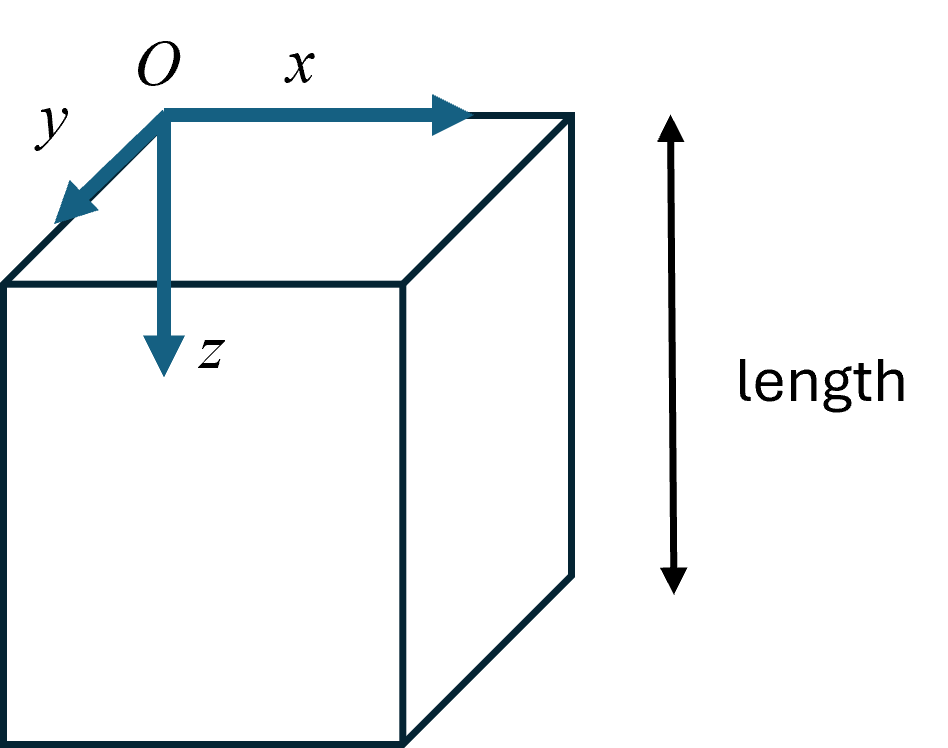
\includegraphics[width=0.3\linewidth]{./figs/geometries/cube.png}
    \caption{Cube parametrization}
    \label{fig:cube}
\end{figure}

As illustrated in Fig.~\ref{fig:cube}, the local coordinate system is defined by the axes $x$, $y$, and $z$, where the origin corresponds to the reference corner of the specimen. The $x$ direction represents the longitudinal direction of the specimen, the $y$ direction represents the transverse thickness direction, and the $z$ direction represents the vertical depth direction.

The cube geometry is defined by the following parameter:

\begin{itemize}
    \item \texttt{length}: side length of the cube.
\end{itemize}


\subsection{\texttt{cylinder}}
\label{subsec:geometry_cylinder}

\begin{figure}[h!]
    \centering
    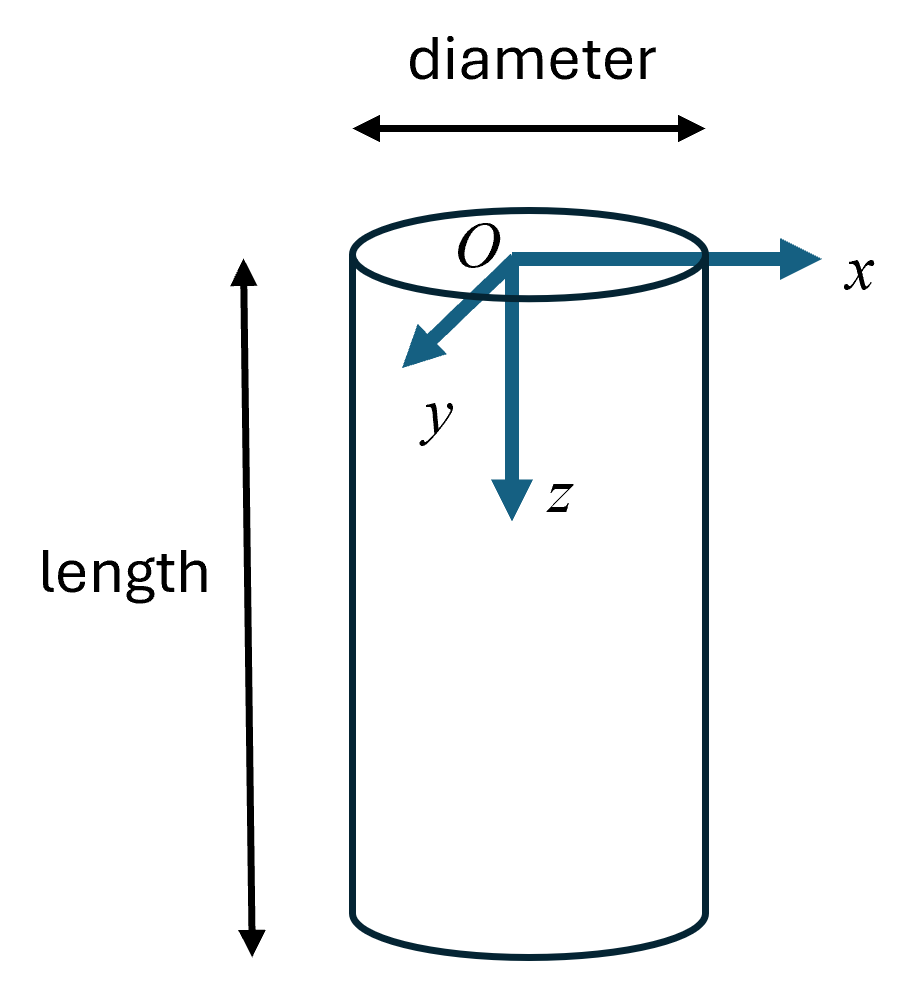
\includegraphics[width=0.3\linewidth]{./figs/geometries/cylinder.png}
    \caption{Cylinder parametrization}
    \label{fig:cylinder}
\end{figure}

As illustrated in Fig.~\ref{fig:cylinder}, the local coordinate system is defined by the axes $x$, $y$, and $z$, where the origin corresponds to the center of the top circular surface of the specimen. The $z$ axis represents the longitudinal direction associated with the cylinder length, while the $x$ and $y$ axes define the transverse directions within the circular cross section.

The cylinder geometry is defined by the following parameters:

\begin{itemize}
    \item \texttt{length}: longitudinal length of the cylinder measured along the $z$ axis;
    \item \texttt{diameter}: diameter of the circular cross section.
\end{itemize}


\subsection{\texttt{double\_notched\_prism}}
\label{subsec:geometry_double_notched_prism}

\begin{figure}[h!]
    \centering
    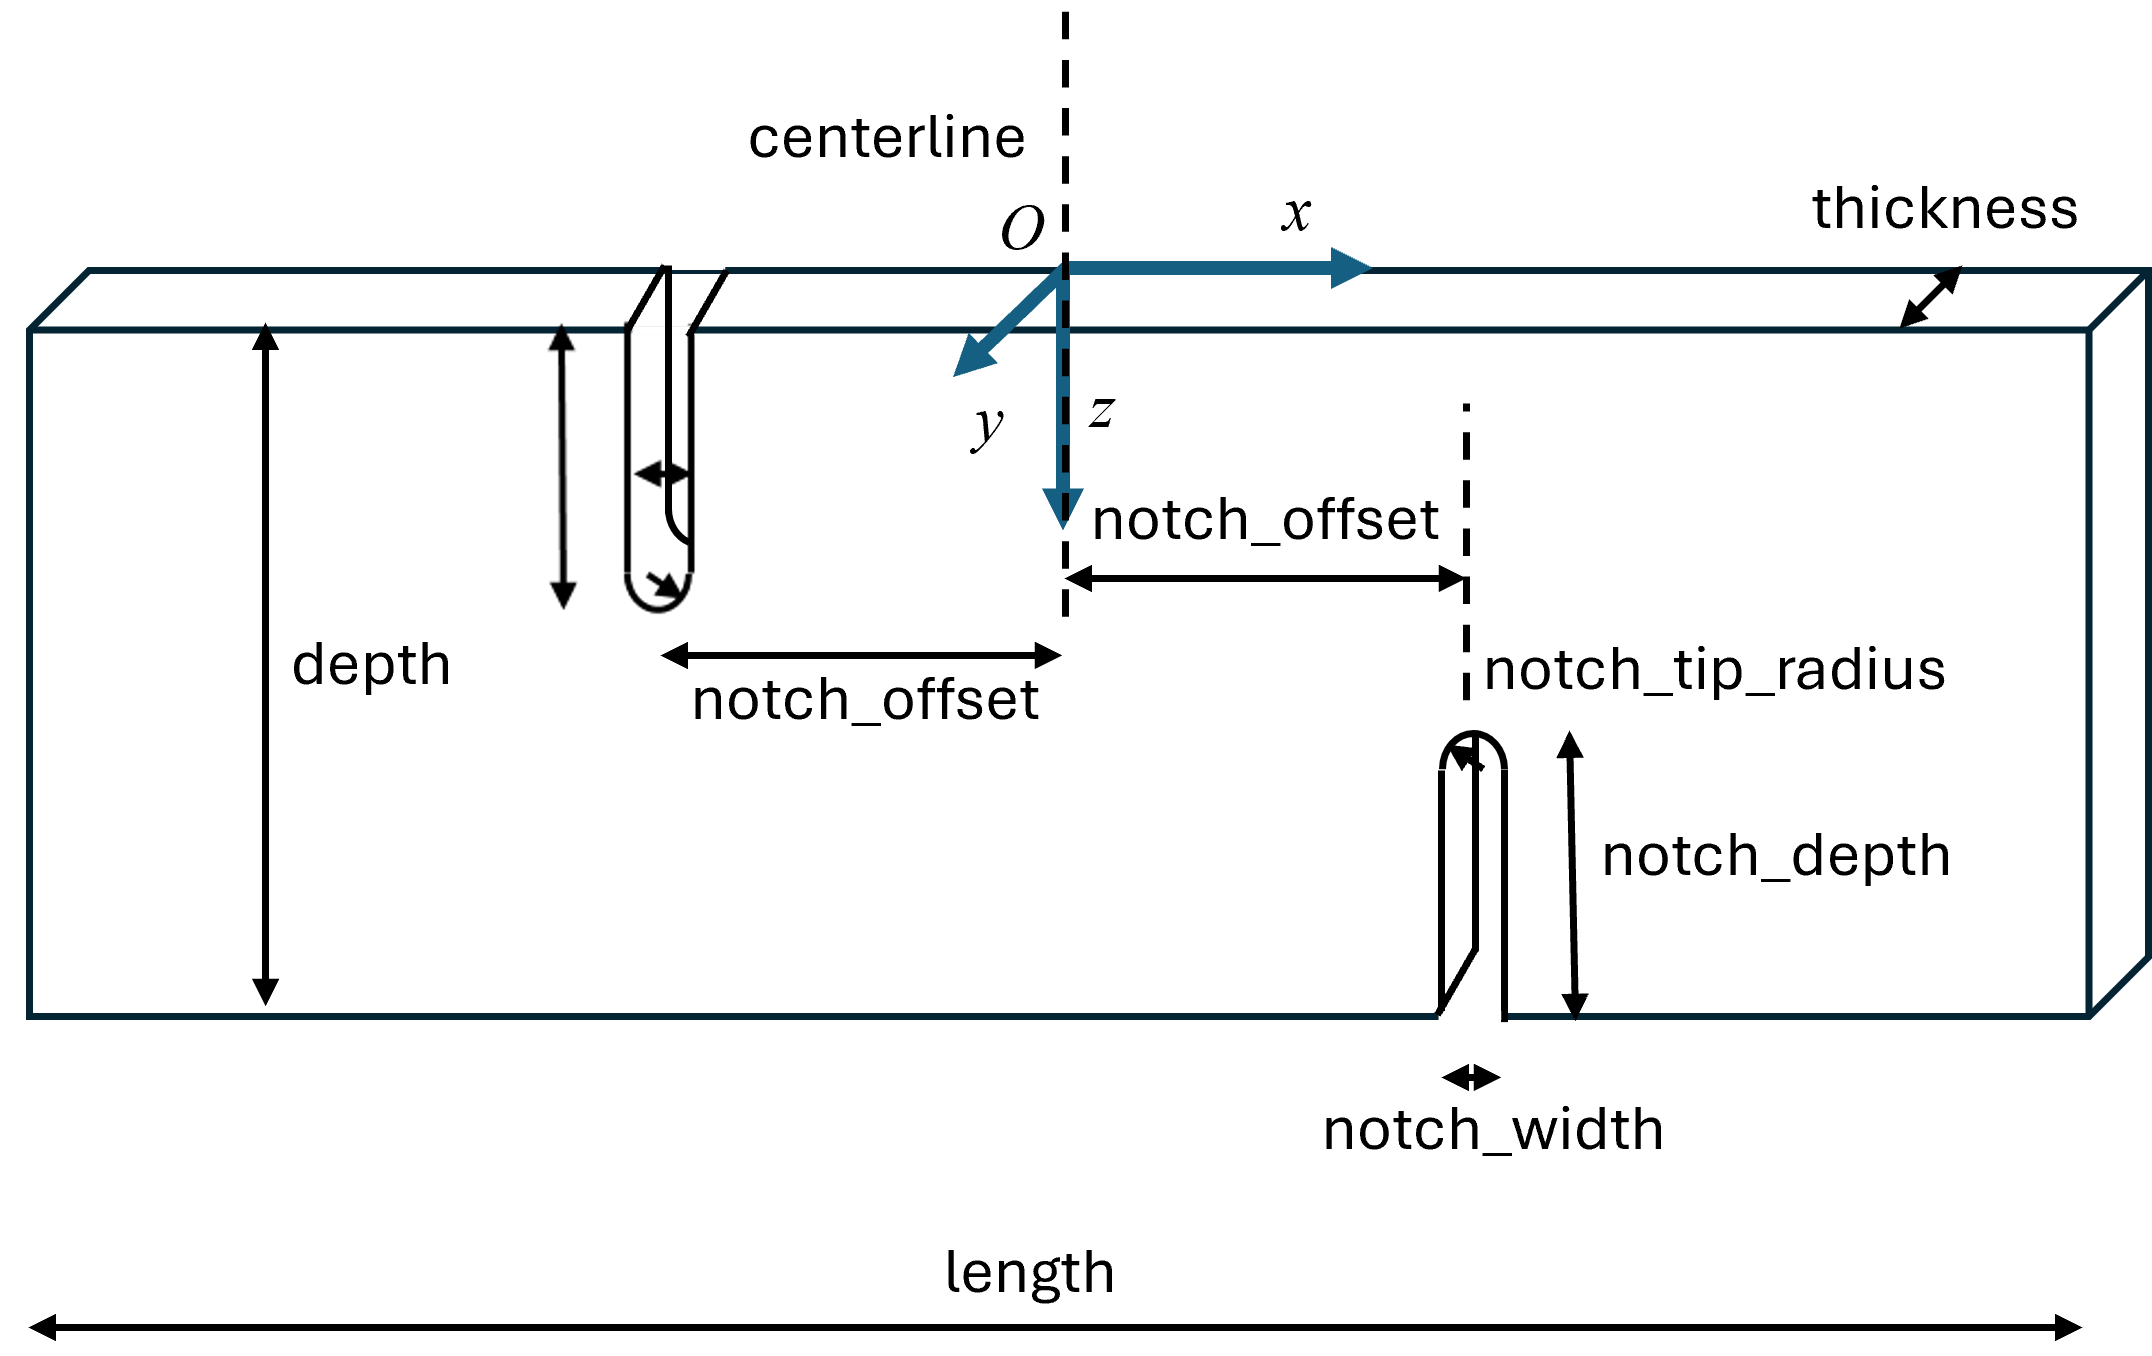
\includegraphics[width=0.6\linewidth]{./figs/geometries/double_notched_prism.png}
    \caption{Doubly notched prism parametrization}
    \label{fig:double_notched_prism}
\end{figure}

As illustrated in Fig.~\ref{fig:double_notched_prism}, the local coordinate system is defined by the axes $x$, $y$, and $z$, where the origin is located on the centerline of the specimen. The $x$ axis represents the longitudinal direction associated with the prism length, the $y$ axis represents the transverse thickness direction, and the $z$ axis represents the vertical depth direction. The two notches are positioned anti-symmetrically relative to the specimen centerline through the parameters \texttt{notch\_offset}.

The double notched prism geometry is defined by the following parameters:

\begin{itemize}
    \item \texttt{length}: prism length measured along the $x$ axis;
    \item \texttt{thickness}: prism thickness measured along the $y$ axis;
    \item \texttt{depth}: prism depth measured along the $z$ axis;
    \item \texttt{notch\_offset}: offset of the first notches relative to the specimen centerline;
    \item \texttt{notch\_depth}: notch penetration depth measured along the $z$ direction;
    \item \texttt{notch\_width}: notch opening width;
    \item \texttt{notch\_tip\_radius}: radius at the notch tip.
\end{itemize}


\subsection{\texttt{dogbone}}
\label{subsec:geometry_dogbone}

\begin{figure}[h!]
    \centering
    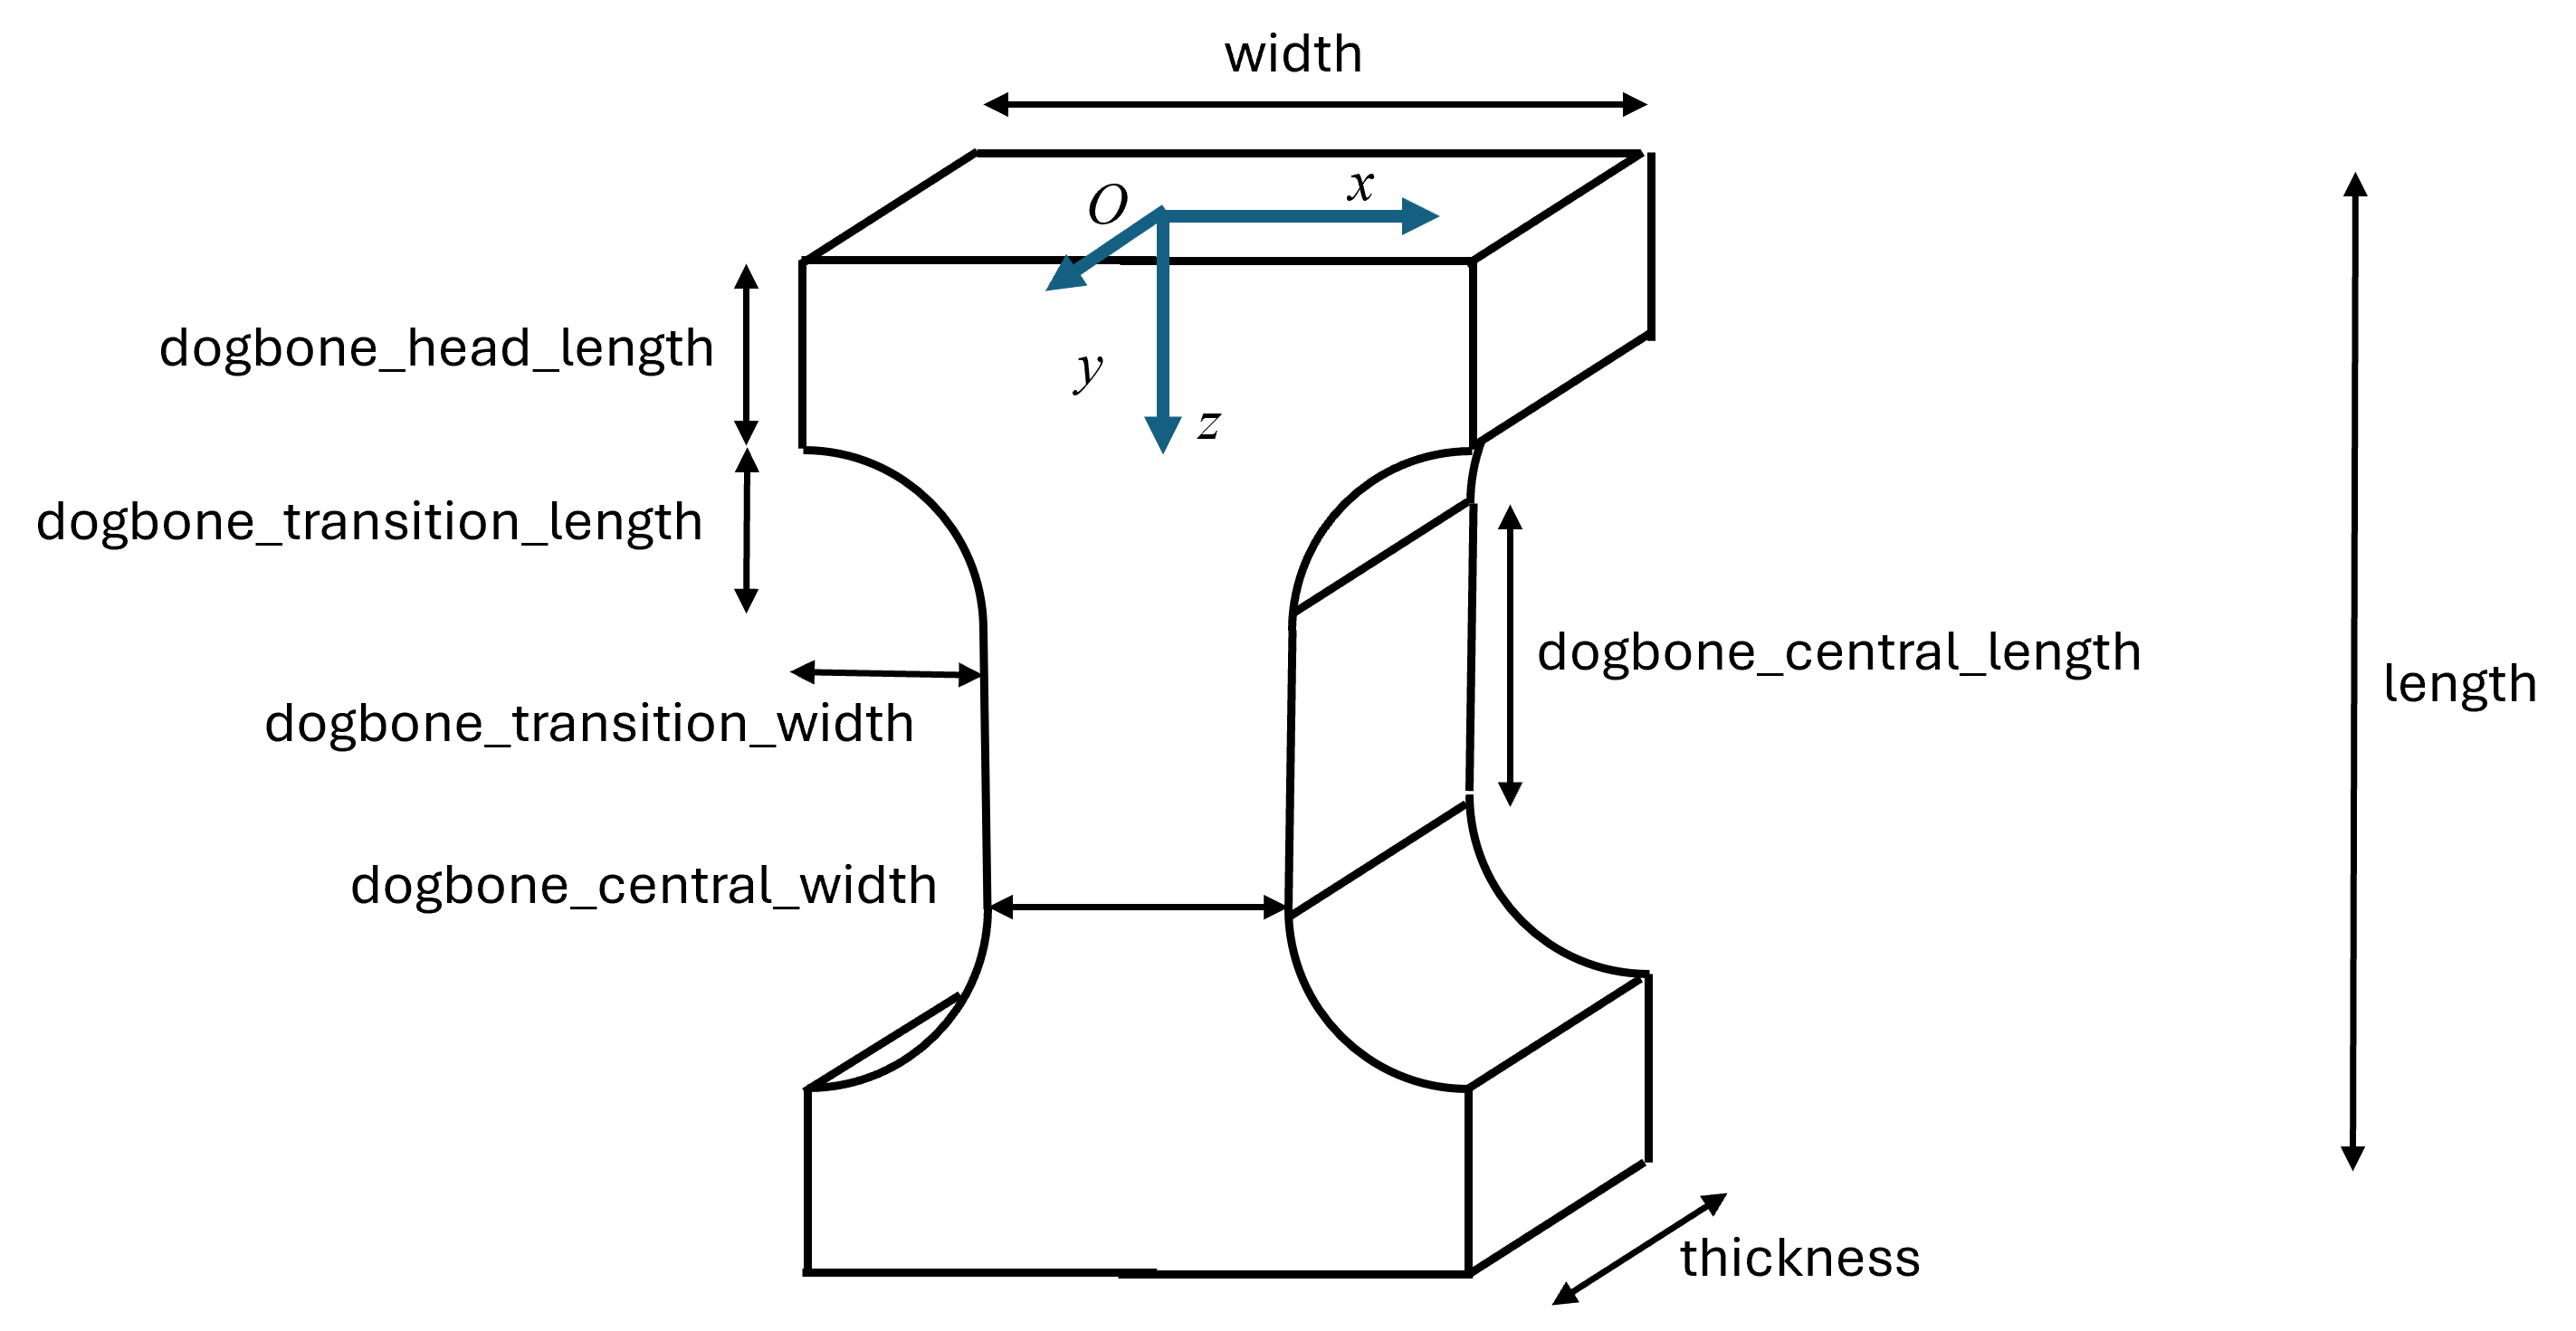
\includegraphics[width=0.6\linewidth]{./figs/geometries/dogbone.png}
    \caption{Dogbone parametrization}
    \label{fig:dogbone}
\end{figure}

As illustrated in Fig.~\ref{fig:dogbone}, the local coordinate system is defined by the axes $x$, $y$, and $z$, where the origin is located on the top side and on the longitudinal axis of symmetry of the specimen. The $z$ axis represents the longitudinal direction associated with the dogbone length, the $y$ axis represents the transverse thickness direction, and the $x$ axis represents the horizontal width direction. The reduced central section of the specimen is defined through the corresponding geometric parameters specified below.

\begin{itemize}
    \item \texttt{length}: total specimen length measured along the $z$ axis;
    \item \texttt{width}: maximum specimen width measured along the $x$ axis;
    \item \texttt{thickness}: specimen thickness measured along the $y$ axis;
    \item \texttt{dogbone\_central\_length}: length of the reduced central region measured along the $z$ axis;
    \item \texttt{dogbone\_central\_width}: width of the reduced central region measured along the $x$ axis;
    \item \texttt{dogbone\_head\_length}: length of each enlarged head region measured along the $z$ axis;
    \item \texttt{dogbone\_transition\_length}: length of each transition region between the head and central regions measured along the $z$ axis;
    \item \texttt{dogbone\_transition\_width}: width variation defining the transition from the head width to the central width measured along the $x$ axis.
\end{itemize}


\subsection{\texttt{notched\_prism}}
\label{subsec:geometry_notched_prism}

\begin{figure}[h!]
    \centering
    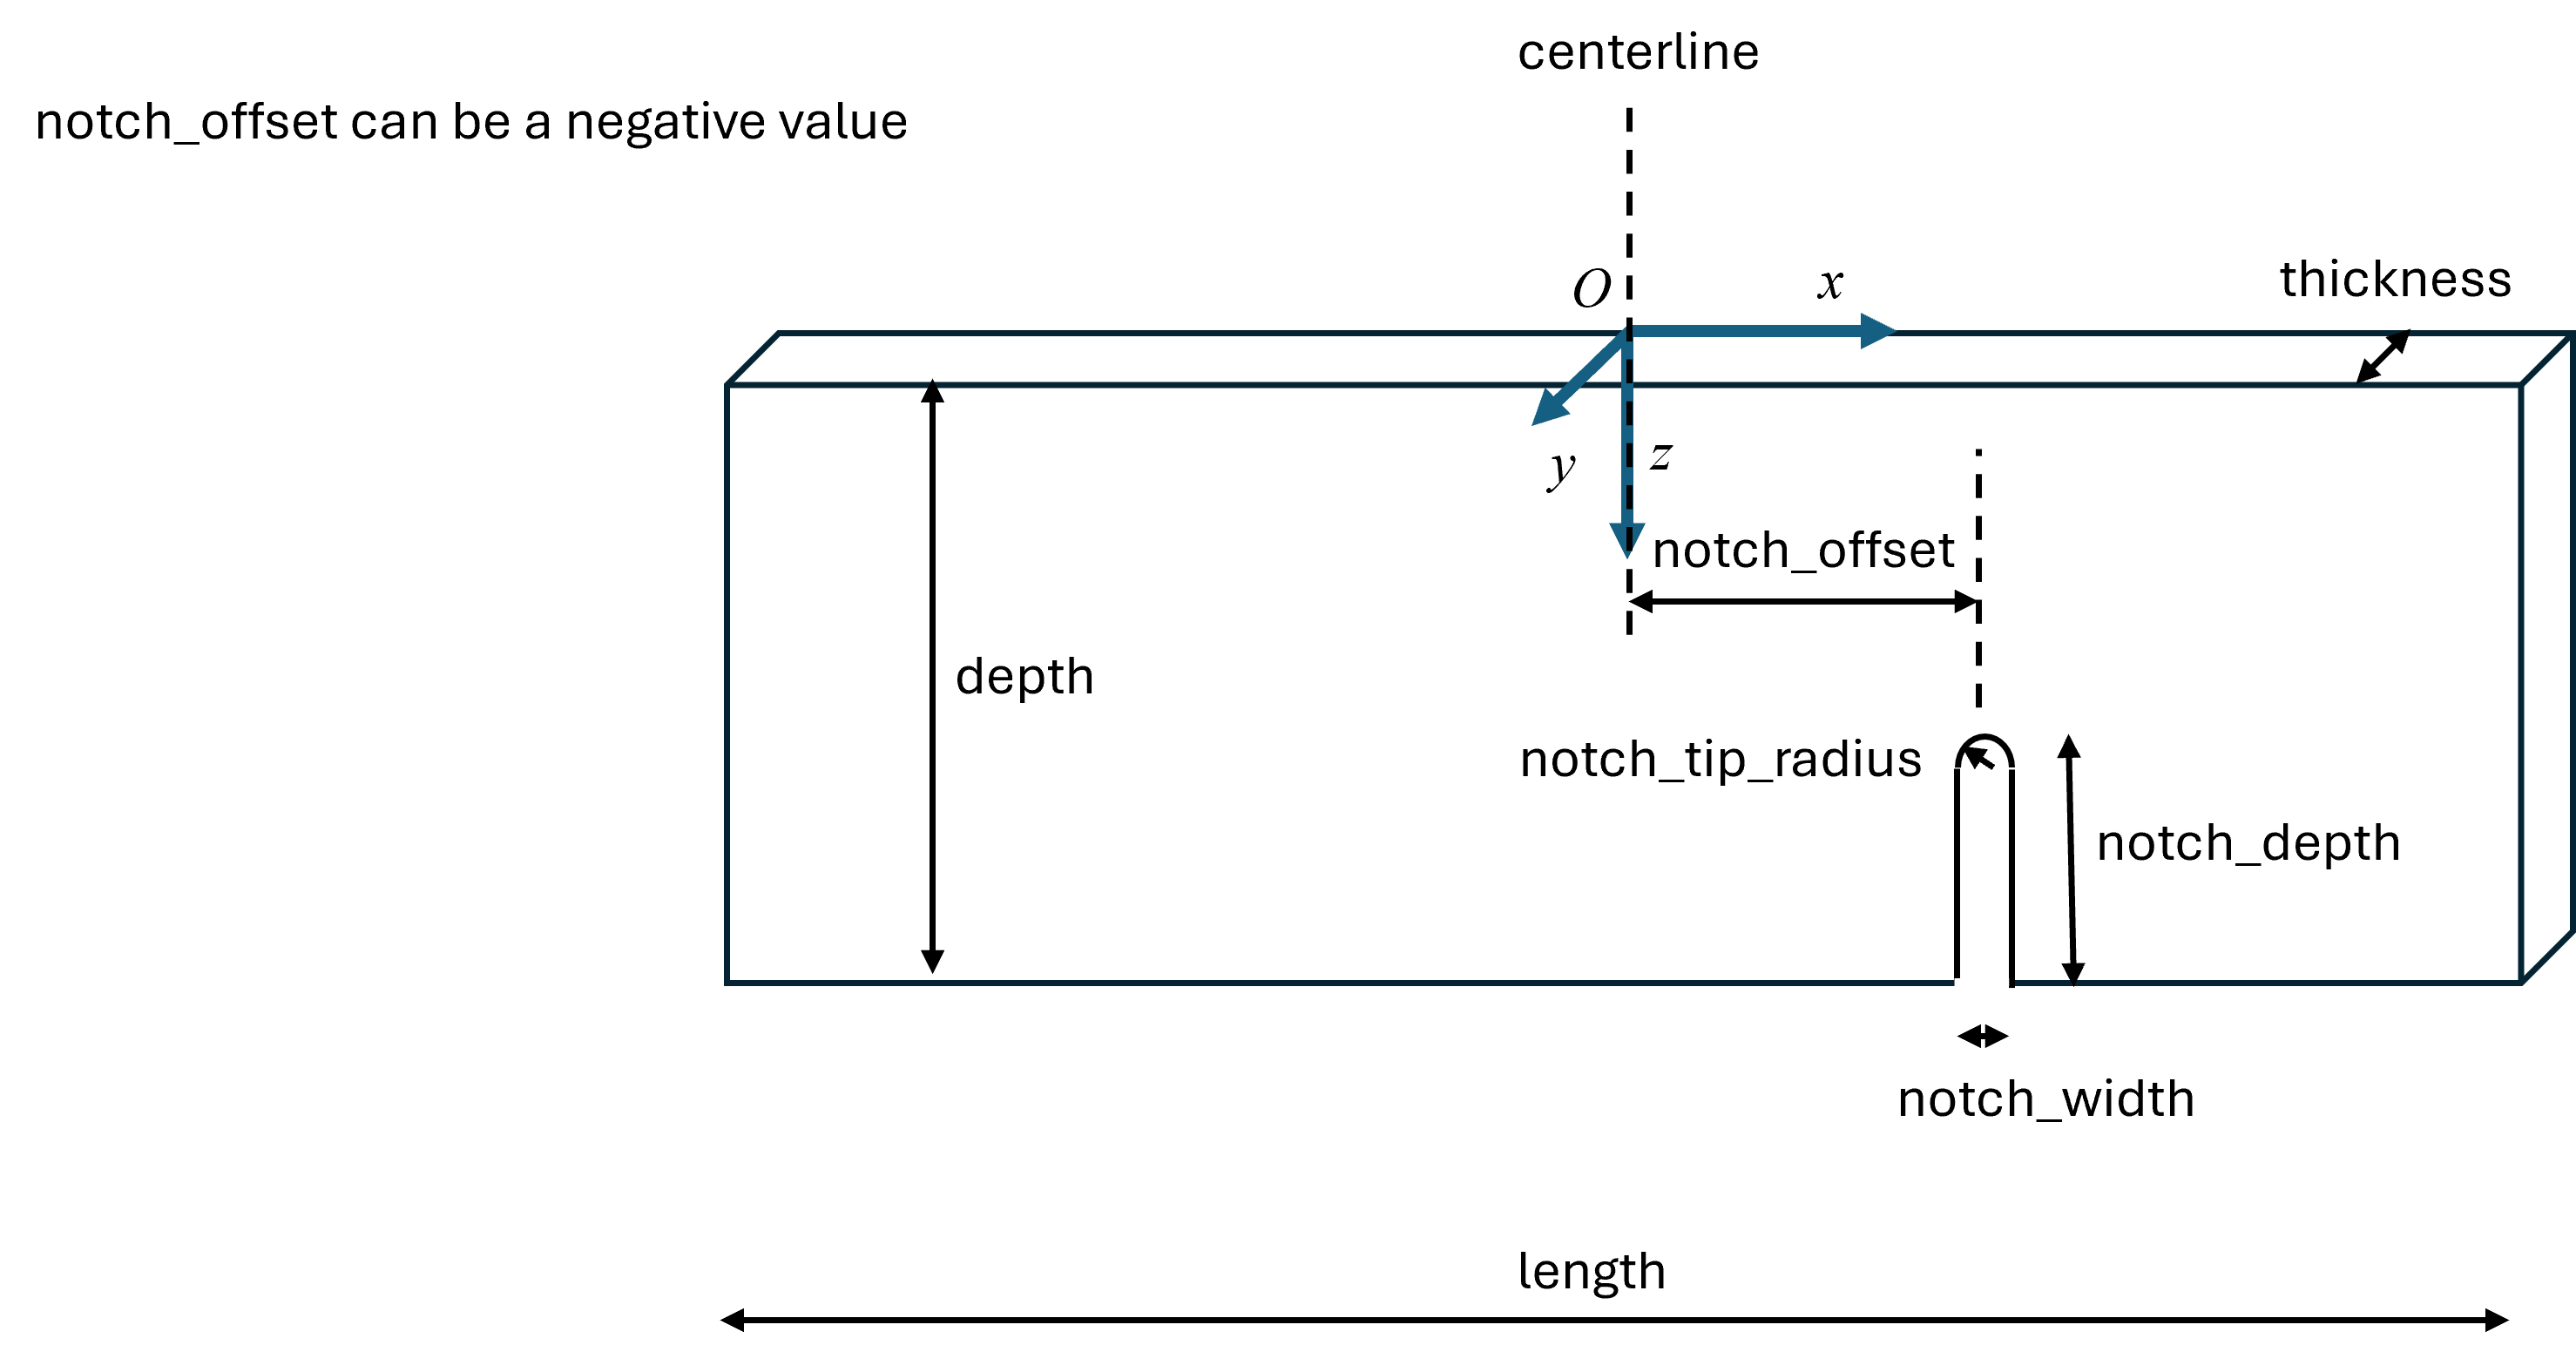
\includegraphics[width=0.6\linewidth]{./figs/geometries/notched_prism.png}
    \caption{Notched prism parametrization}
    \label{fig:notched_prism}
\end{figure}

As illustrated in Fig.~\ref{fig:notched_prism}, the local coordinate system is defined by the axes $x$, $y$, and $z$, where the origin corresponds to the reference corner of the specimen. The $x$ axis represents the longitudinal direction associated with the prism length, the $y$ axis represents the transverse thickness direction, and the $z$ axis represents the vertical depth direction. The notch is positioned relative to the specimen centerline through the parameter \texttt{notch\_offset}. \texttt{notch\_offset} can be either positive or negative.

The notched prism geometry is defined by the following parameters:

\begin{itemize}
    \item \texttt{length}: prism length measured along the $x$ axis;
    \item \texttt{thickness}: prism thickness measured along the $y$ axis;
    \item \texttt{depth}: prism depth measured along the $z$ axis;
    \item \texttt{notch\_offset}: offset of the notch relative to the specimen centerline;
    \item \texttt{notch\_depth}: notch penetration depth measured along the $z$ direction;
    \item \texttt{notch\_width}: notch opening width;
    \item \texttt{notch\_tip\_radius}: radius at the notch tip.
\end{itemize}


\subsection{\texttt{ell\_shape}}
\label{subsec:geometry_ell_shape}

\begin{figure}[h!]
    \centering
    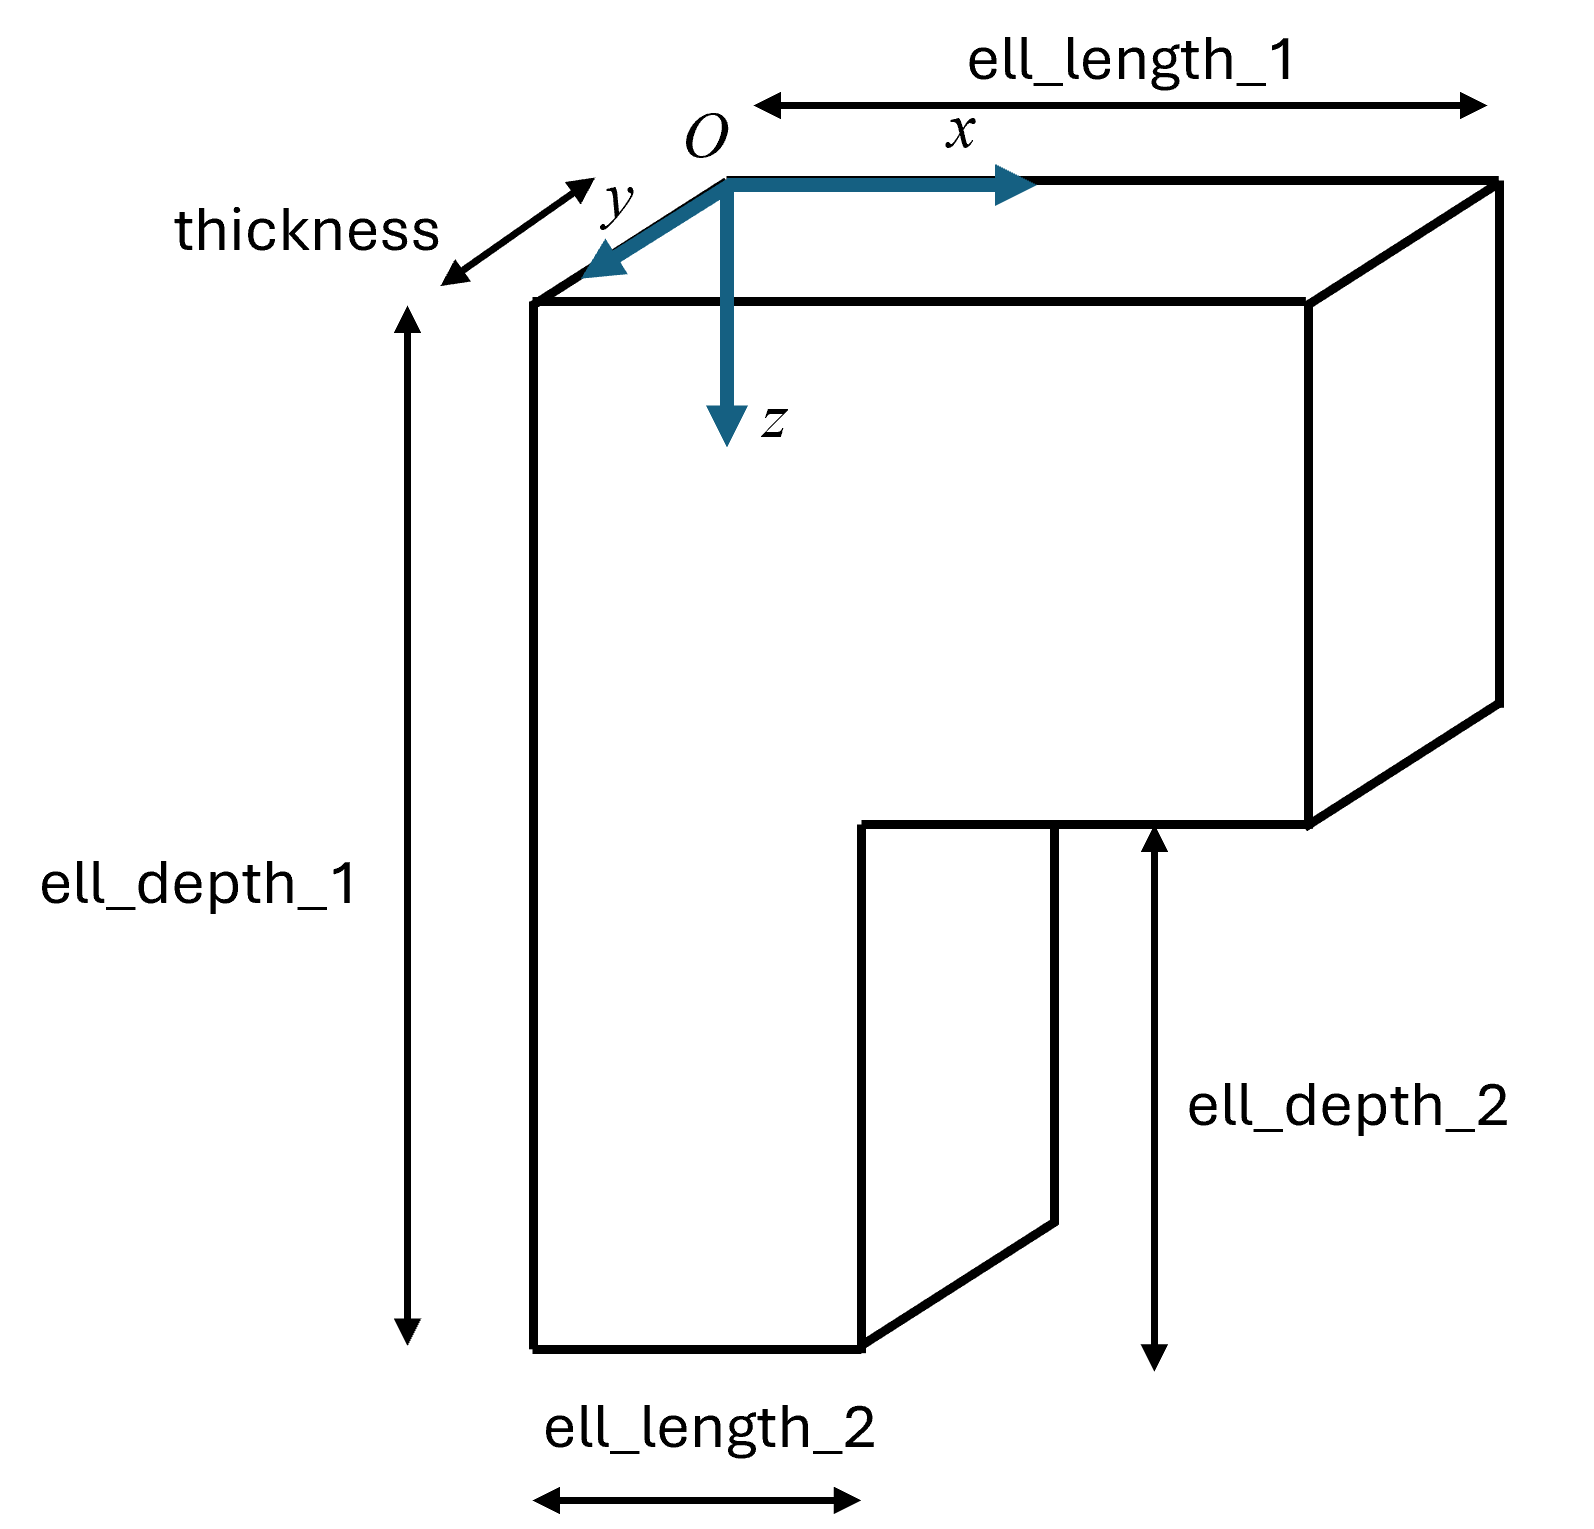
\includegraphics[width=0.5\linewidth]{./figs/geometries/ell_shape.png}
    \caption{Ell shape parametrization}
    \label{fig:ell_shape}
\end{figure}

As illustrated in Fig.~\ref{fig:ell_shape}, the local coordinate system is defined by the axes $x$, $y$, and $z$, where the origin corresponds to the reference corner of the specimen. The $x$ axis represents the longitudinal direction of the specimen, the $y$ axis represents the transverse thickness direction, and the $z$ axis represents the vertical depth direction. The L-shaped geometry is defined through the corresponding geometric parameters specified in the geometry parametrization library.

The ell-shape geometry is defined by the following parameters:

As illustrated in Fig.~\ref{fig:ell_shape}, the local coordinate system is defined by the axes $x$, $y$, and $z$, where the origin corresponds to the reference corner of the specimen. The $x$ axis represents the longitudinal direction of the specimen, the $y$ axis represents the transverse thickness direction, and the $z$ axis represents the vertical depth direction. The L-shaped geometry is defined through the corresponding geometric parameters specified below.

\begin{itemize}
    \item \texttt{ell\_depth\_1}: depth of the vertical branch measured along the $z$ axis;
    \item \texttt{ell\_depth\_2}: depth of the horizontal branch measured along the $z$ axis;
    \item \texttt{ell\_length\_1}: length of the horizontal branch measured along the $x$ axis;
    \item \texttt{ell\_length\_2}: length of the vertical branch measured along the $x$ axis;
    \item \texttt{thickness}: specimen thickness measured along the $y$ axis.
\end{itemize}


\subsection{\texttt{notched\_cylinder}}
\label{subsec:geometry_notched_cylinder}

\begin{figure}[h!]
    \centering
    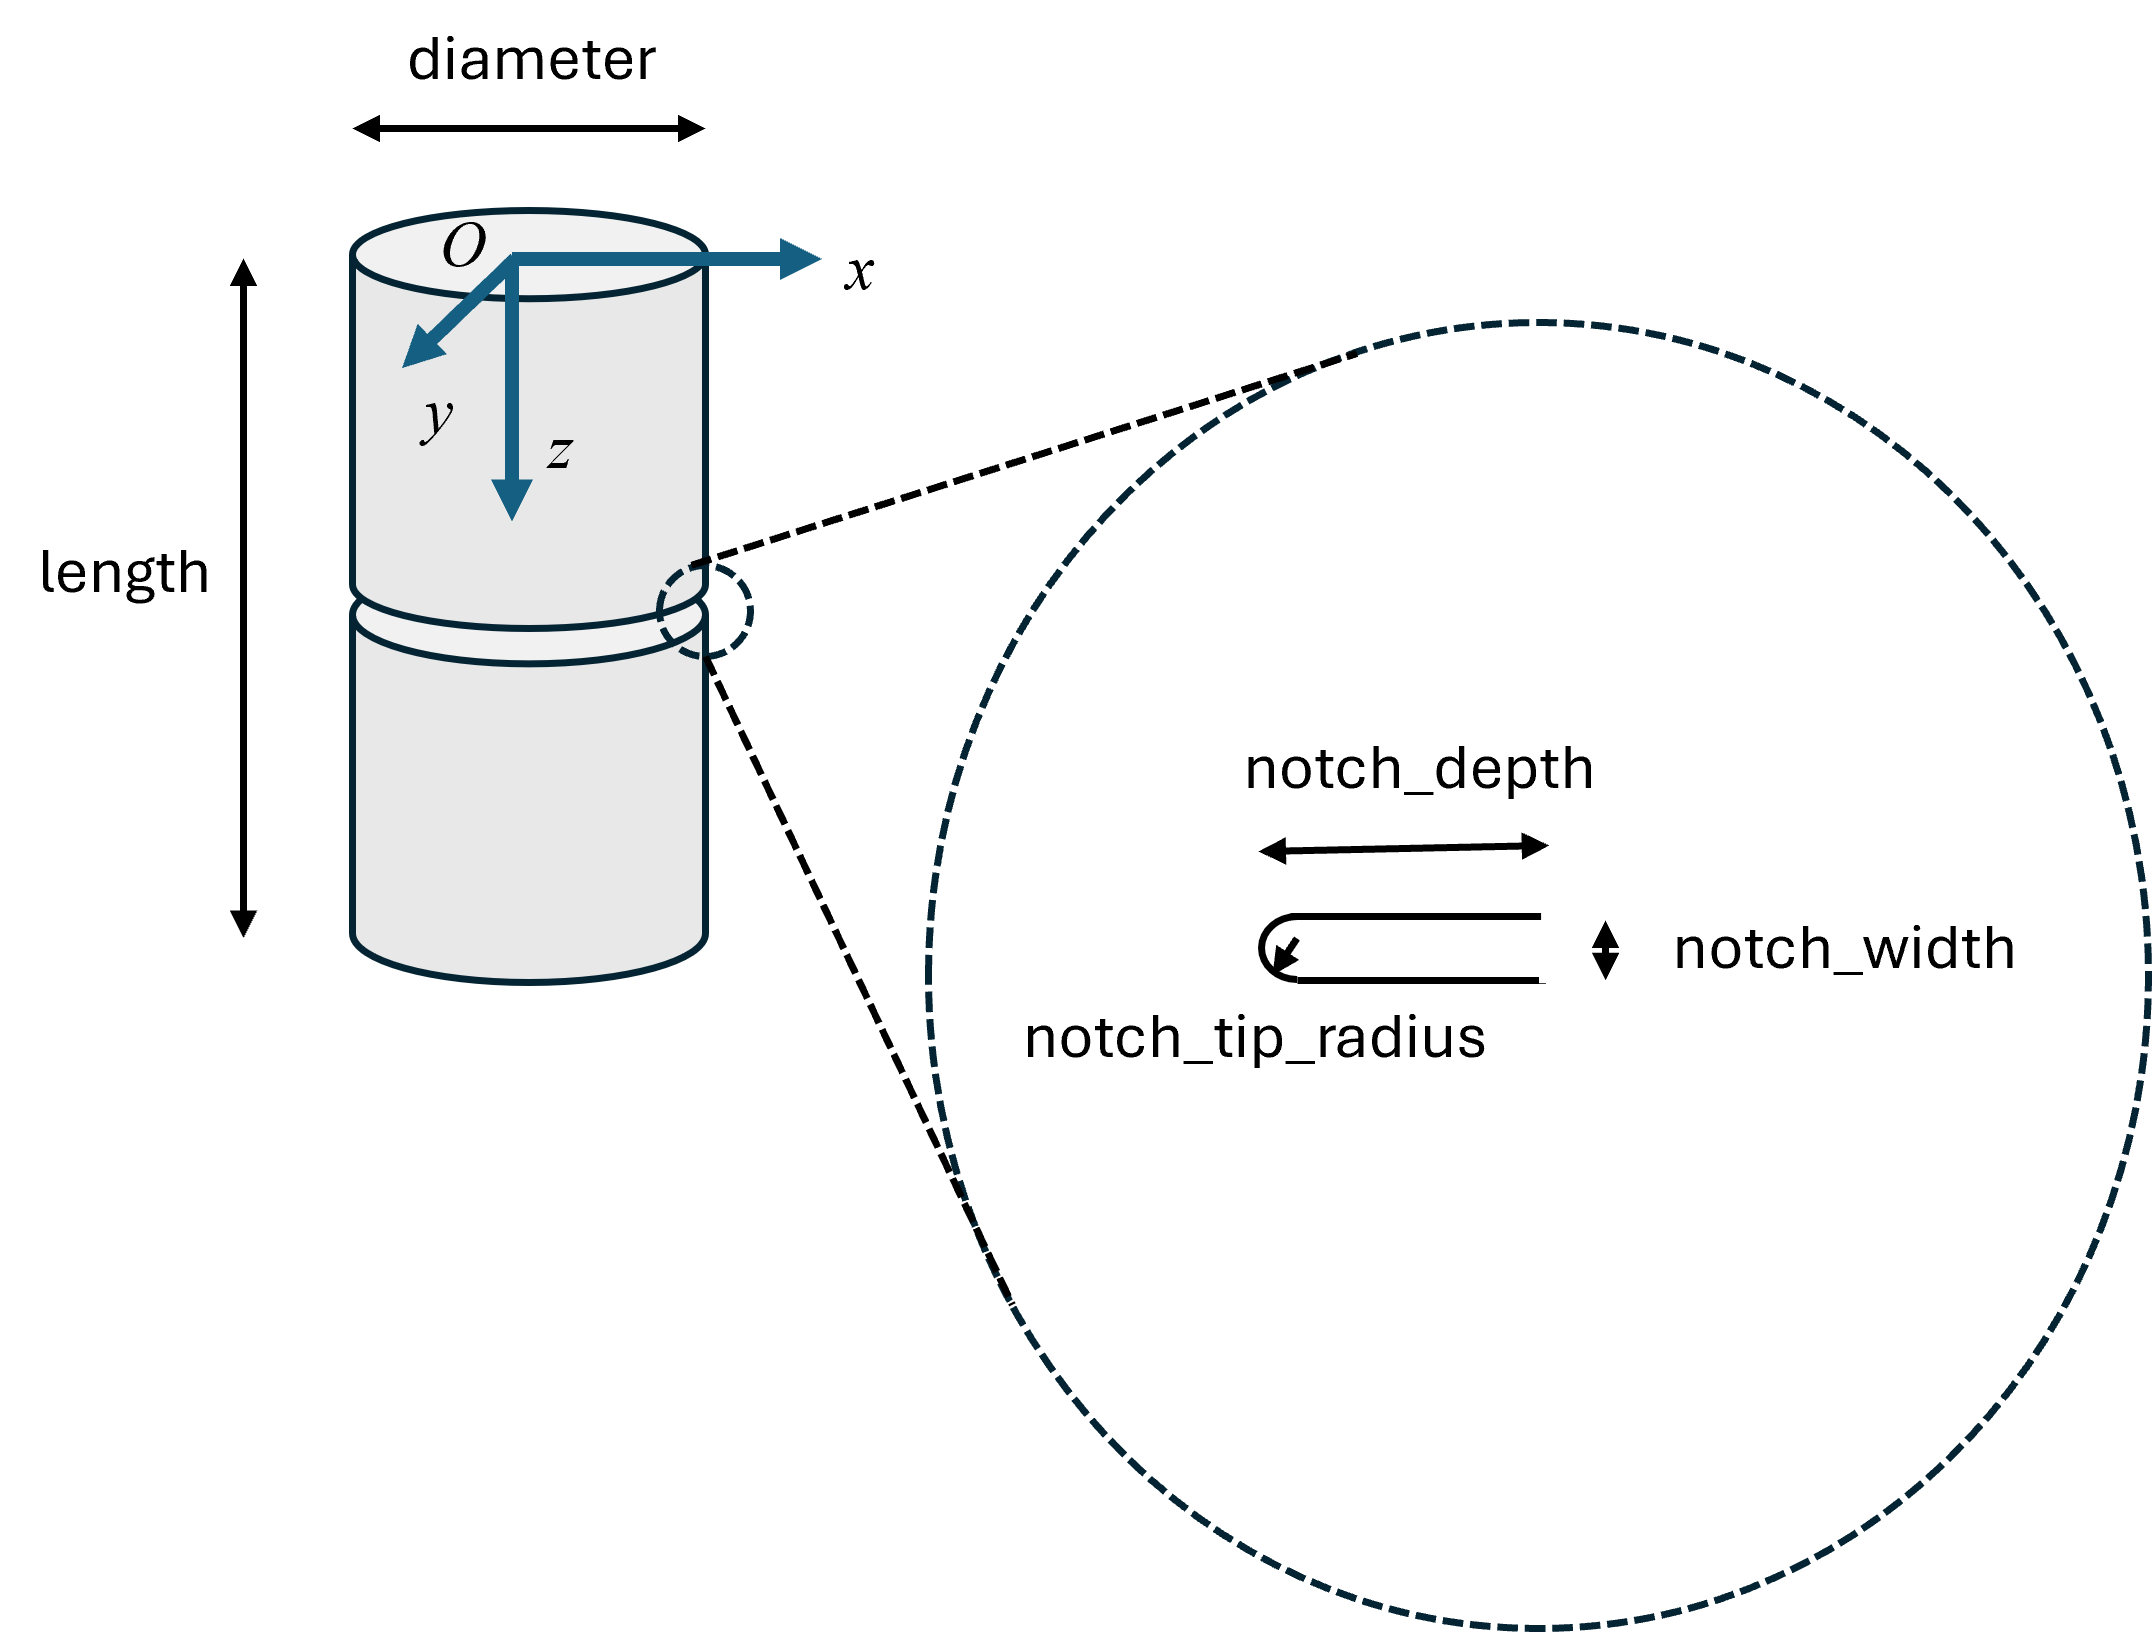
\includegraphics[width=0.6\linewidth]{./figs/geometries/notched_cylinder.png}
    \caption{Notched cylinder parametrization}
    \label{fig:notched_cylinder}
\end{figure}

As illustrated in Fig.~\ref{fig:notched_cylinder}, the local coordinate system is defined by the axes $x$, $y$, and $z$, where the origin corresponds to the center of the top circular surface of the specimen. The $z$ axis represents the longitudinal direction associated with the cylinder length, while the $x$ and $y$ axes define the transverse directions within the circular cross section. The circumferential notch is positioned along the cylinder axis at mid-length.


The notched cylinder geometry is defined by the following parameters:

\begin{itemize}
    \item \texttt{length}: longitudinal length of the cylinder measured along the $z$ axis;
    \item \texttt{diameter}: diameter of the circular cross section;
    \item \texttt{notch\_depth}: radial notch depth;
    \item \texttt{notch\_width}: axial width of the circumferential notch;
    \item \texttt{notch\_tip\_radius}: radius at the notch tip.
\end{itemize}


\subsection{\texttt{prism}}
\label{subsec:geometry_prism}

\begin{figure}[h!]
    \centering
    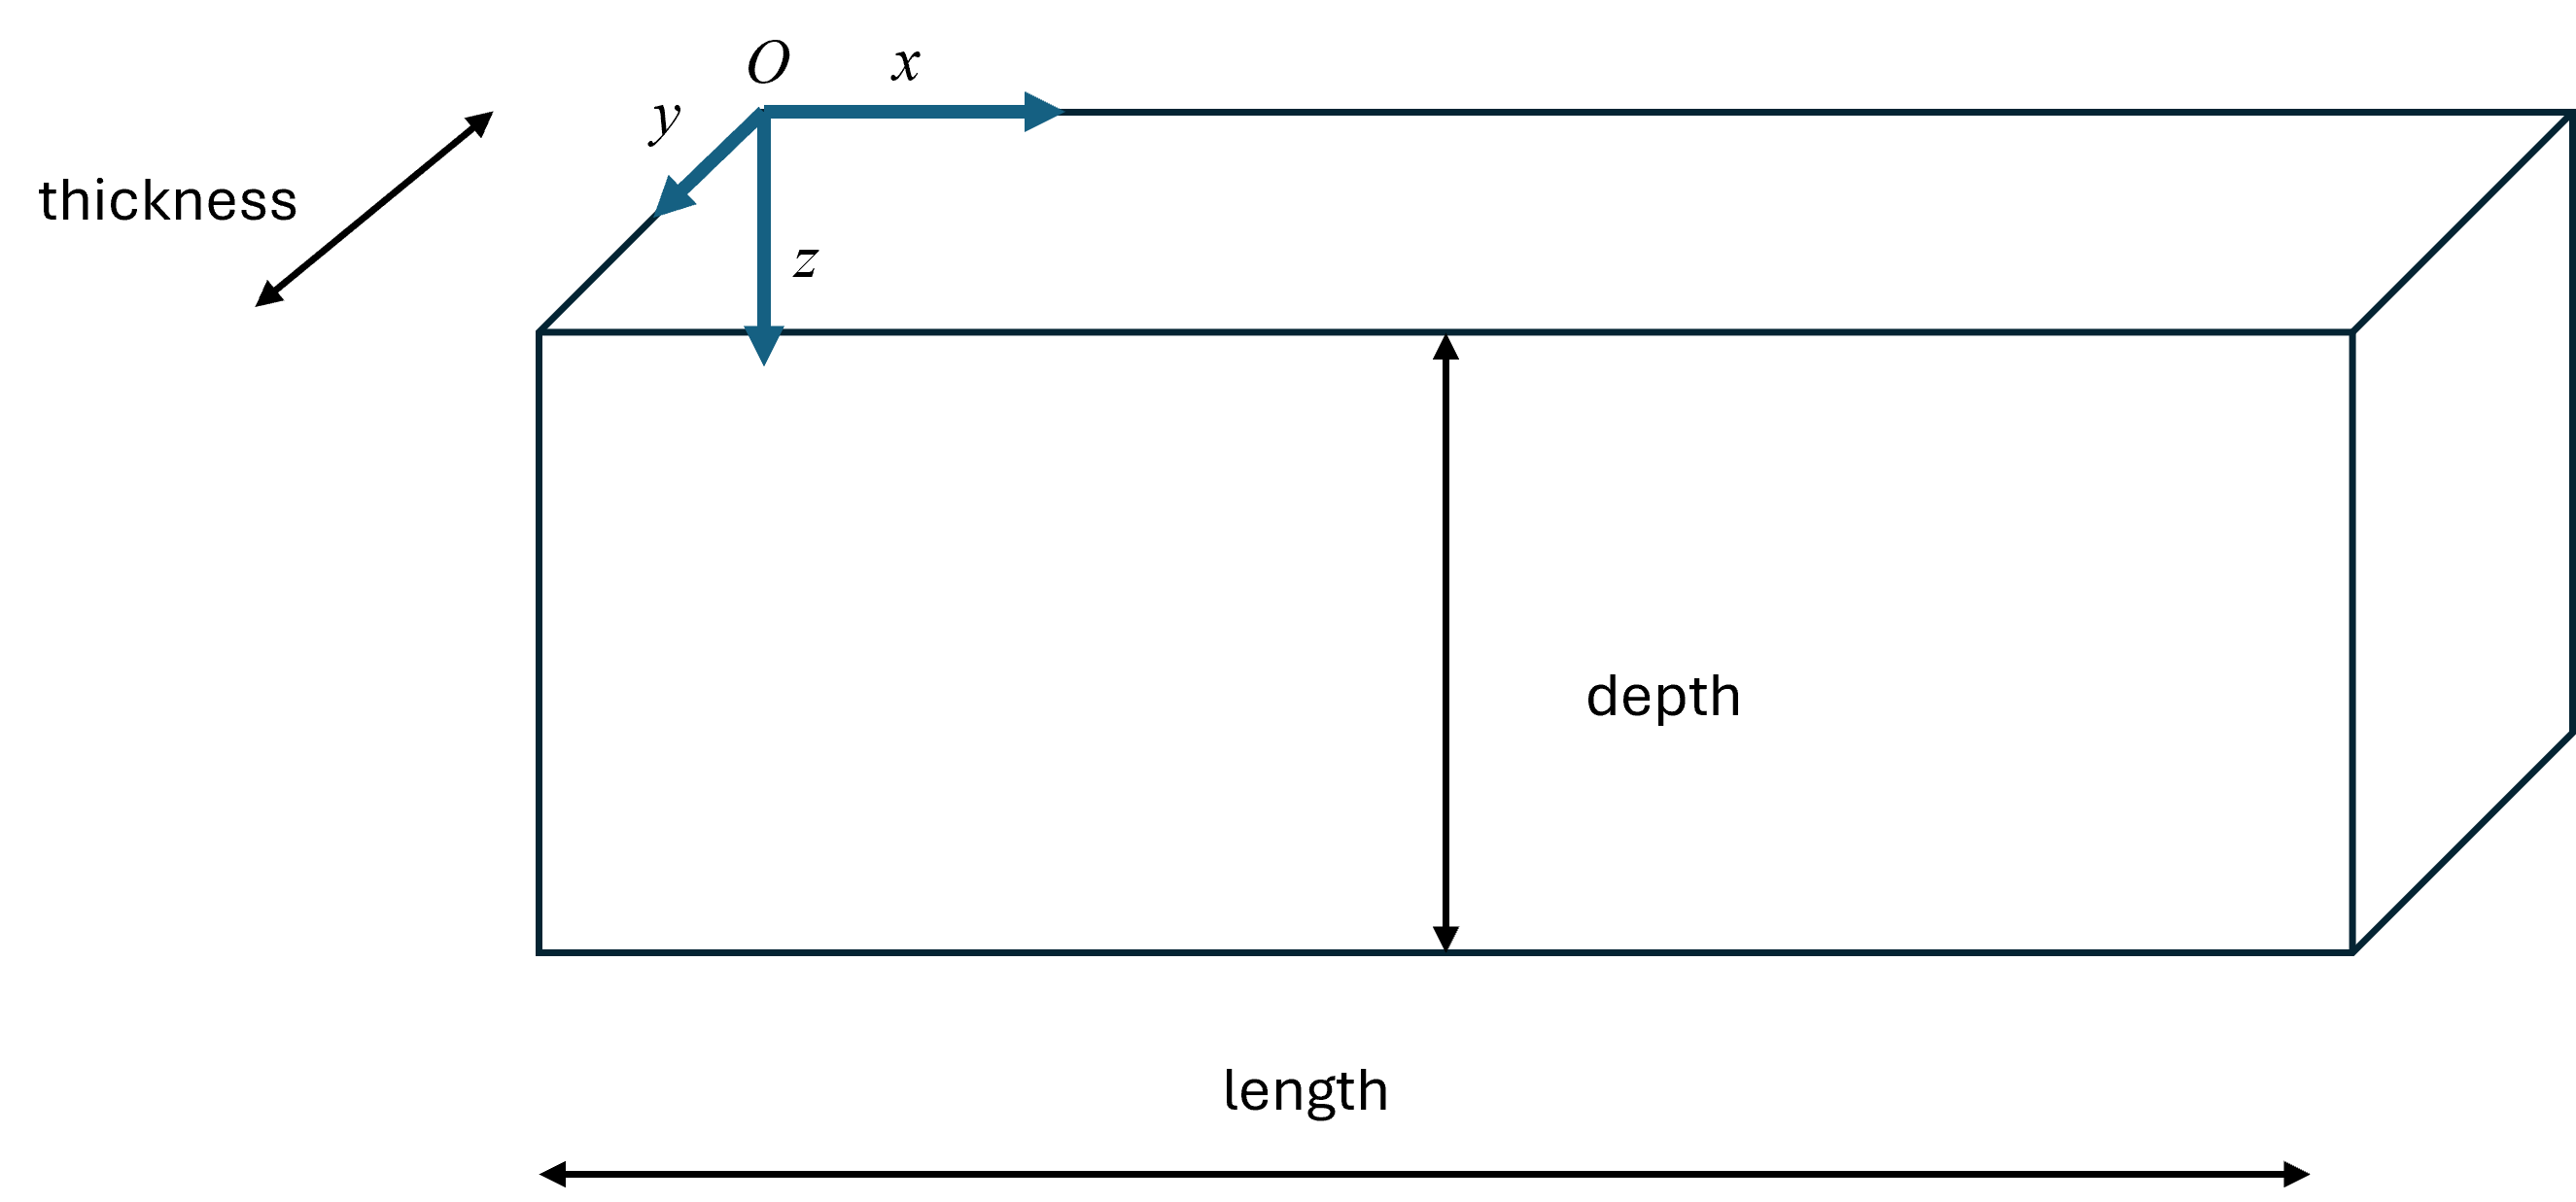
\includegraphics[width=0.7\linewidth]{./figs/geometries/prism.png}
    \caption{Prism parametrization}
    \label{fig:prism}
\end{figure}

As illustrated in Fig.~\ref{fig:prism}, the local coordinate system is defined by the axes $x$, $y$, and $z$, where the origin corresponds to the reference corner of the specimen. The $x$ axis represents the longitudinal direction associated with the prism length, the $y$ axis represents the transverse thickness direction, and the $z$ axis represents the vertical depth direction.

The prism geometry is defined by the following parameters:

\begin{itemize}
    \item \texttt{length}: prism length measured along the $x$ axis;
    \item \texttt{thickness}: prism thickness measured along the $y$ axis;
    \item \texttt{depth}: prism depth measured along the $z$ axis.
\end{itemize}









\newpage
\section{Reinforcement Geometry Parametrization Library}
The Reinforcement Parametrization Library defines the standardized parametric representations used to describe the geometry of reinforcement configurations throughout the database. The library provides canonical parametrizations for longitudinal tensile and flexural reinforcement, transverse reinforcement systems such as stirrups and ties, and externally bonded or externally attached reinforcement systems. Each reinforcement type is described through a consistent set of geometric descriptors, coordinate conventions, orientation definitions, spacing parameters, and material-property descriptors referenced to the Cartesian coordinate system associated with the corresponding specimen geometry.

The adopted geometrical parametrizations are designed to balance simplicity, extensibility, machine readability, and practical usability while capturing the dominant reinforcement characteristics required for structural interpretation, computational modeling, database interoperability, and future AI-assisted workflows. Rather than reproducing every local geometric detail of reinforcement bending shapes, hooks, laps, or anchorage configurations, the library focuses on the principal geometric and mechanical descriptors most relevant for simulation, model calibration, model validation, and systematic comparison across datasets. When more detailed representations are necessary, contributors may supplement the parametrized descriptions with additional drawings, CAD files, annotated figures, photographs, or auxiliary reinforcement description files.


The current reinforcement parametrization schemes and coordinate conventions are described below.

\subsection{Parametrization of Flexural Reinforcement, Tensile Reinforcement, Stirrups, and Ties}

The reinforcement parametrization adopted for flexural reinforcement, tensile reinforcement, stirrups, and ties is based on a standardized layer-based representation intended to describe reinforcement layouts commonly encountered in reinforced concrete specimens and structural members. The same parametrization can be used for longitudinal reinforcement oriented along the $x$, $y$, or $z$ directions as well as for transverse reinforcement systems such as stirrups and ties.



Each reinforcement entry represents either:

\begin{itemize}
    \item one reinforcement layer containing multiple longitudinal bars;
    \item one set of stirrups or ties repeated at a specified spacing.
\end{itemize}

The reinforcement layout is defined through the following parameters:

\begin{itemize}

    \item \texttt{number}: number of reinforcement bars, stirrups, or ties represented by the entry;

    \item \texttt{bar\_designation}: standard reinforcement designation according to the relevant standard or nomenclature system. The \texttt{other} option may be used for non-standard reinforcement;

    \item \texttt{bar\_nominal\_diameter\_mm}: nominal diameter of the reinforcement element;

    \item \texttt{bar\_nominal\_area\_mm2}: nominal cross-sectional area of the reinforcement element;

    \item \texttt{layer\_depth\_mm}: depth of the reinforcement layer measured from the reference specimen surface. This parameter may be omitted for stirrups and ties;

    \item \texttt{spacing\_mm}: center-to-center spacing between reinforcement elements. For longitudinal reinforcement, this parameter defines the spacing between adjacent bars within a layer. For stirrups and ties, it defines the longitudinal spacing between consecutive transverse reinforcement elements;

    \item \texttt{horizontal\_cover\_mm}: concrete cover measured along the horizontal direction of the specimen coordinate system;

    \item \texttt{vertical\_cover\_mm}: concrete cover measured along the vertical direction of the specimen coordinate system;

    \item \texttt{begin\_distance\_mm}: distance from the specimen origin to the beginning of the reinforcement system along the principal reinforcement direction;

    \item \texttt{end\_distance\_mm}: distance from the specimen origin to the end of the reinforcement system along the principal reinforcement direction.

\end{itemize}

For tensile and flexural reinforcement, the reinforcement bars are assumed to be equally spaced within the reinforcement layer according to the specified \texttt{spacing\_mm}. The combination of layer depth, spacing, cover distances, and begin/end distances defines the position and extent of the reinforcement layer within the specimen.


Figure~\ref{fig:longitudinal_reinf} illustrates the coordinate conventions and principal geometric descriptors adopted for longitudinal flexural and tensile reinforcement layers.

\begin{figure}[htbp]
    \centering
    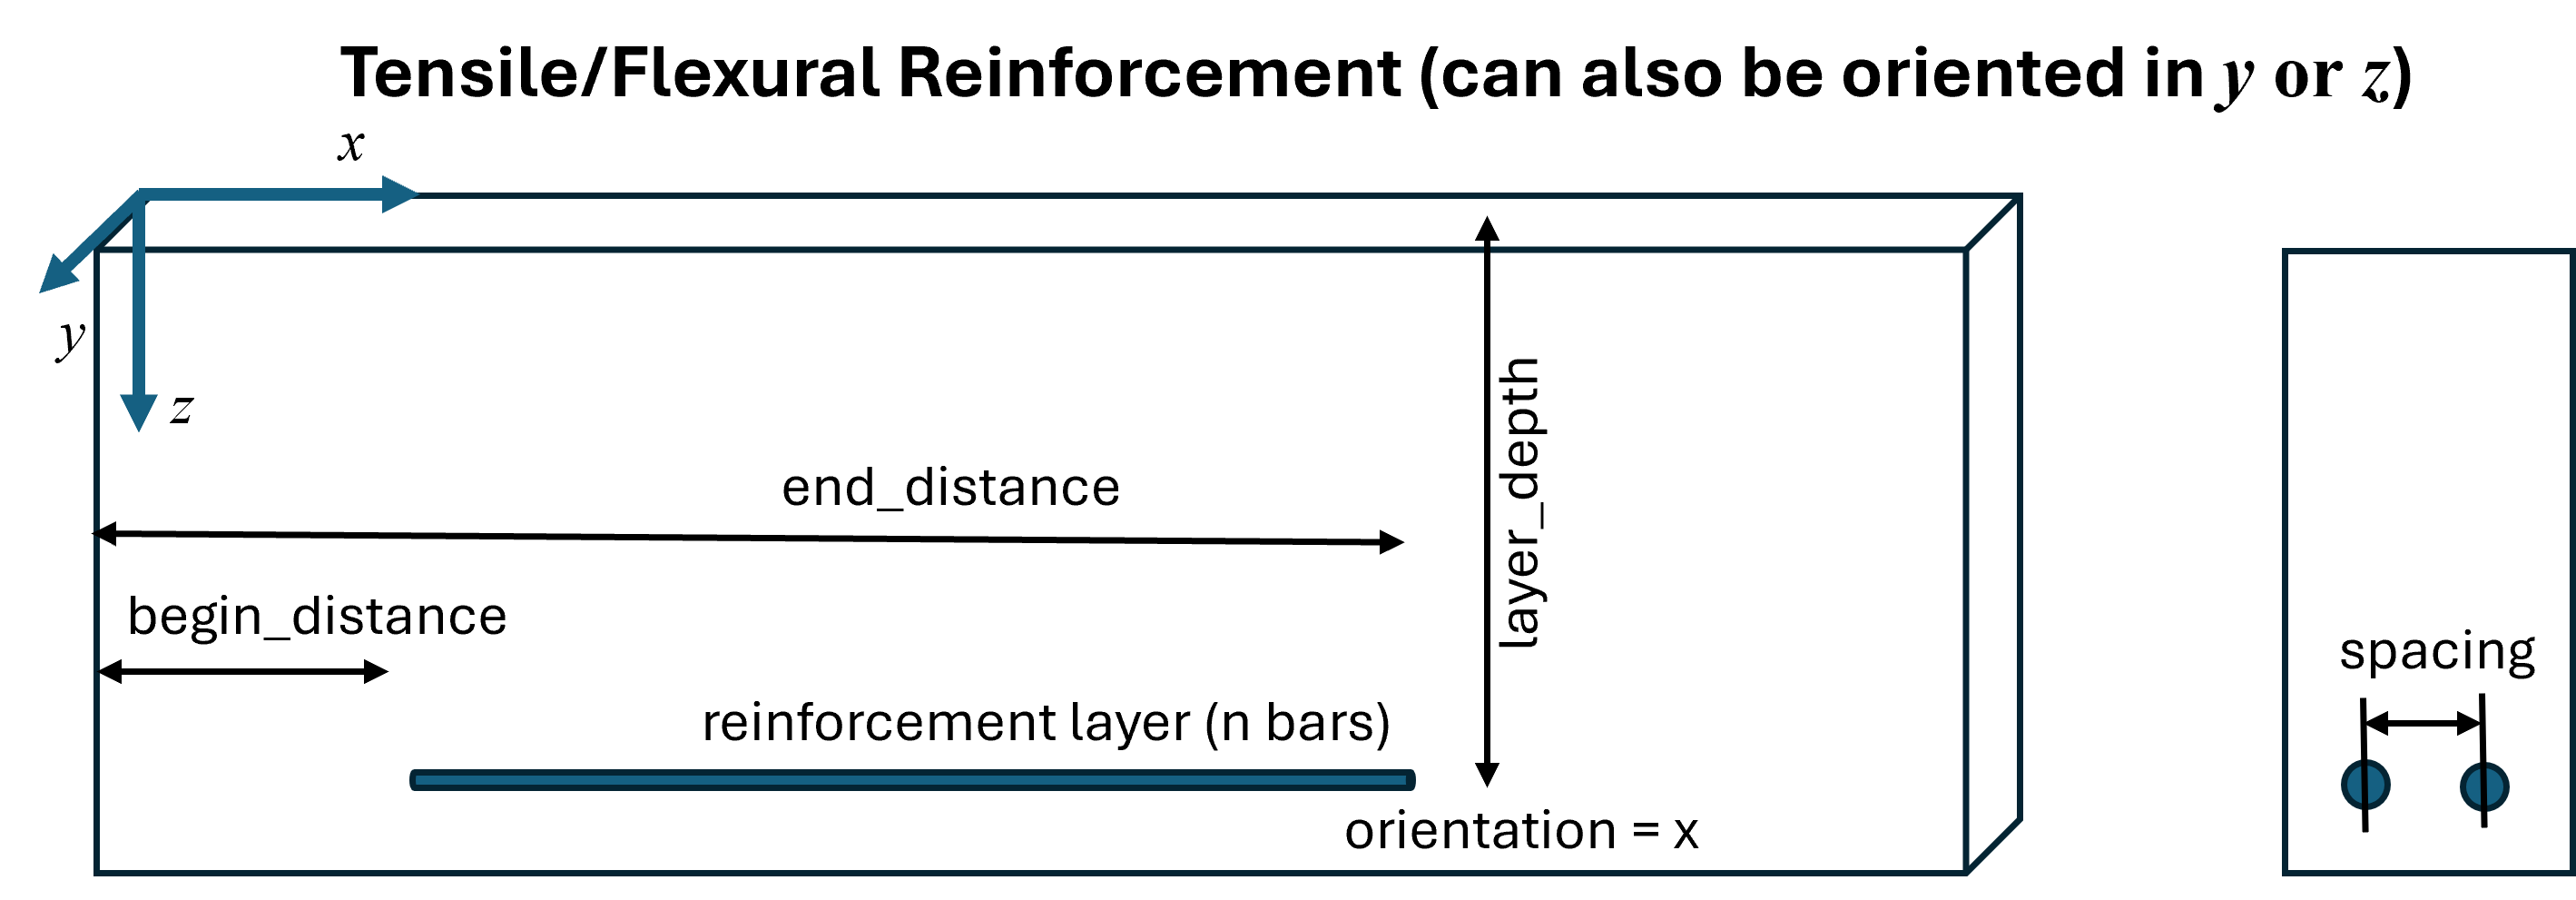
\includegraphics[width=\textwidth]{./figs/reinforcements/longitudinal.png}
    \caption{Parametrization of longitudinal flexural and tensile reinforcement layers.}
    \label{fig:longitudinal_reinf}
\end{figure}

For stirrups and ties, the reinforcement entry represents a repeated transverse reinforcement configuration distributed along the member longitudinal direction. The parameter \texttt{spacing\_mm} defines the center-to-center longitudinal spacing between consecutive stirrups or ties, while \texttt{begin\_distance\_mm} and \texttt{end\_distance\_mm} define the region of the structural member over which the transverse reinforcement is present.


Figure~\ref{fig:stirrups_reinf} illustrates the parametrization adopted for stirrups and ties.

\begin{figure}[htbp]
    \centering
    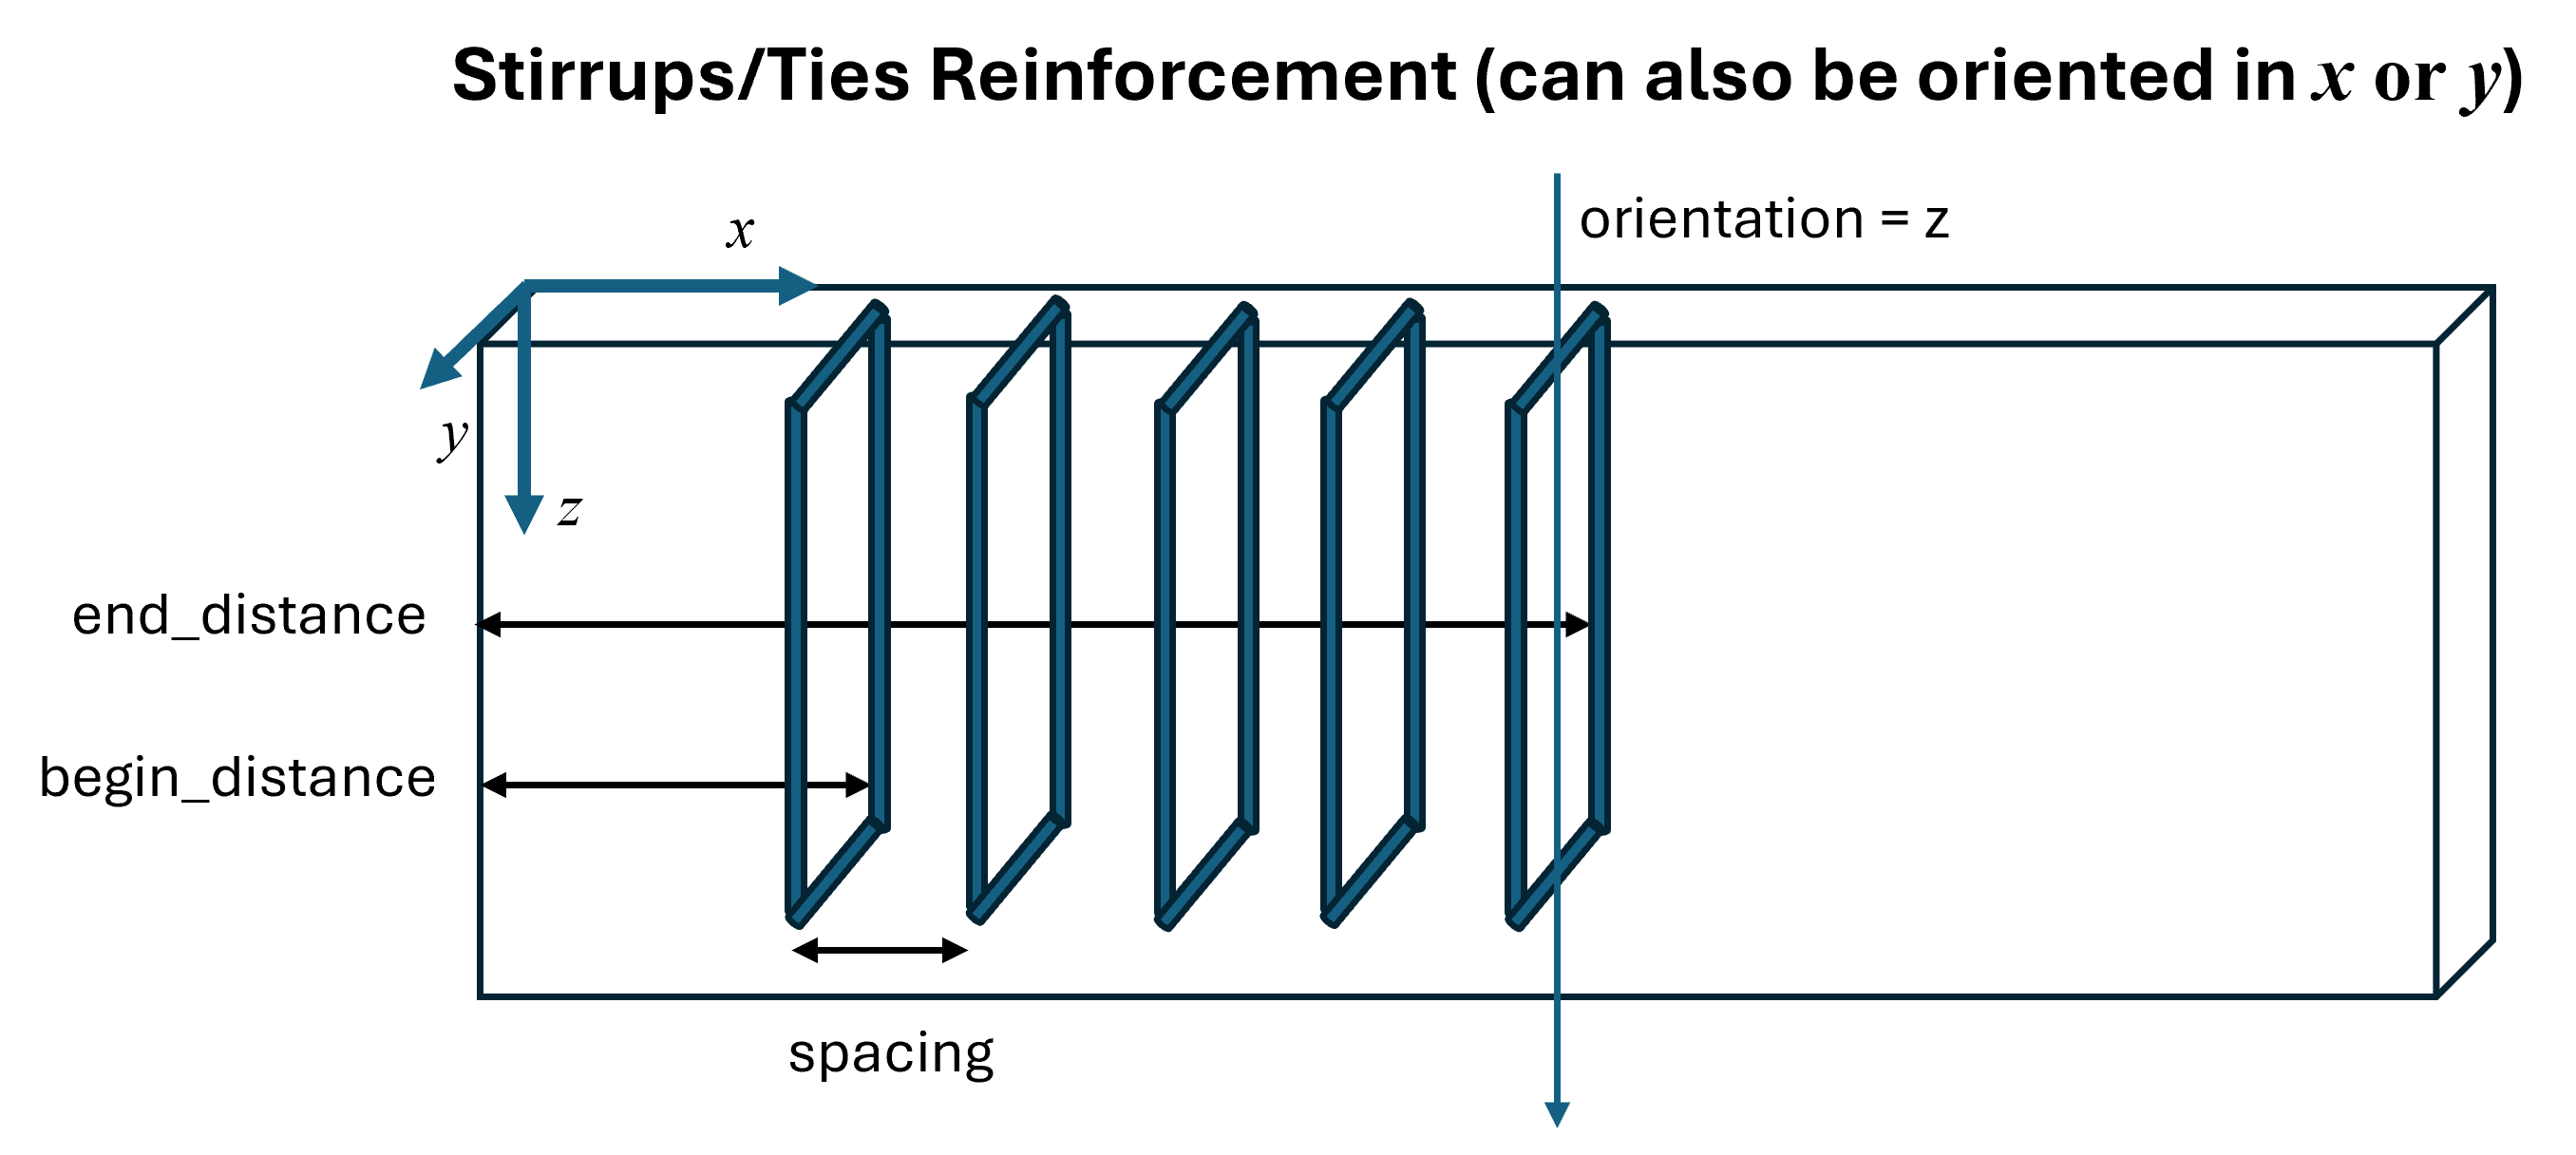
\includegraphics[width=\textwidth]{./figs/reinforcements/stirrups.png}
    \caption{Parametrization of stirrups and ties reinforcement systems.}
    \label{fig:stirrups_reinf}
\end{figure}


\newpage
\section{Parametrization of External Reinforcement}

The current parametrization adopted for externally bonded or externally attached reinforcement systems provides a simplified geometric representation intended primarily for machine readability. The parametrization is currently designed for typical externally bonded reinforcement systems such as FRP laminates, steel plates, externally bonded sheets, strips, and similar reinforcement components applied to the surface of structural members.

The current scheme is admittedly limited and focuses only on the dominant geometric descriptors required to identify the reinforcement location, orientation, dimensions, and some limited anchorage characteristics. The parametrization does not attempt to reproduce detailed local geometries, tapering effects, multilayer stacking sequences, corner wrapping details, fiber orientations within composite laminates, or complex anchorage systems. The library is expected to evolve over time, and future versions will include more advanced parametrizations capable of representing a broader range of externally bonded and externally attached reinforcement configurations.

The current parametrization is illustrated in Fig.~\ref{fig:external_reinf}. The external reinforcement system is represented through a planar reinforcement region characterized by its centroid location, dimensions, orientation, and optional anchorage information.

\begin{figure}[htbp]
    \centering
    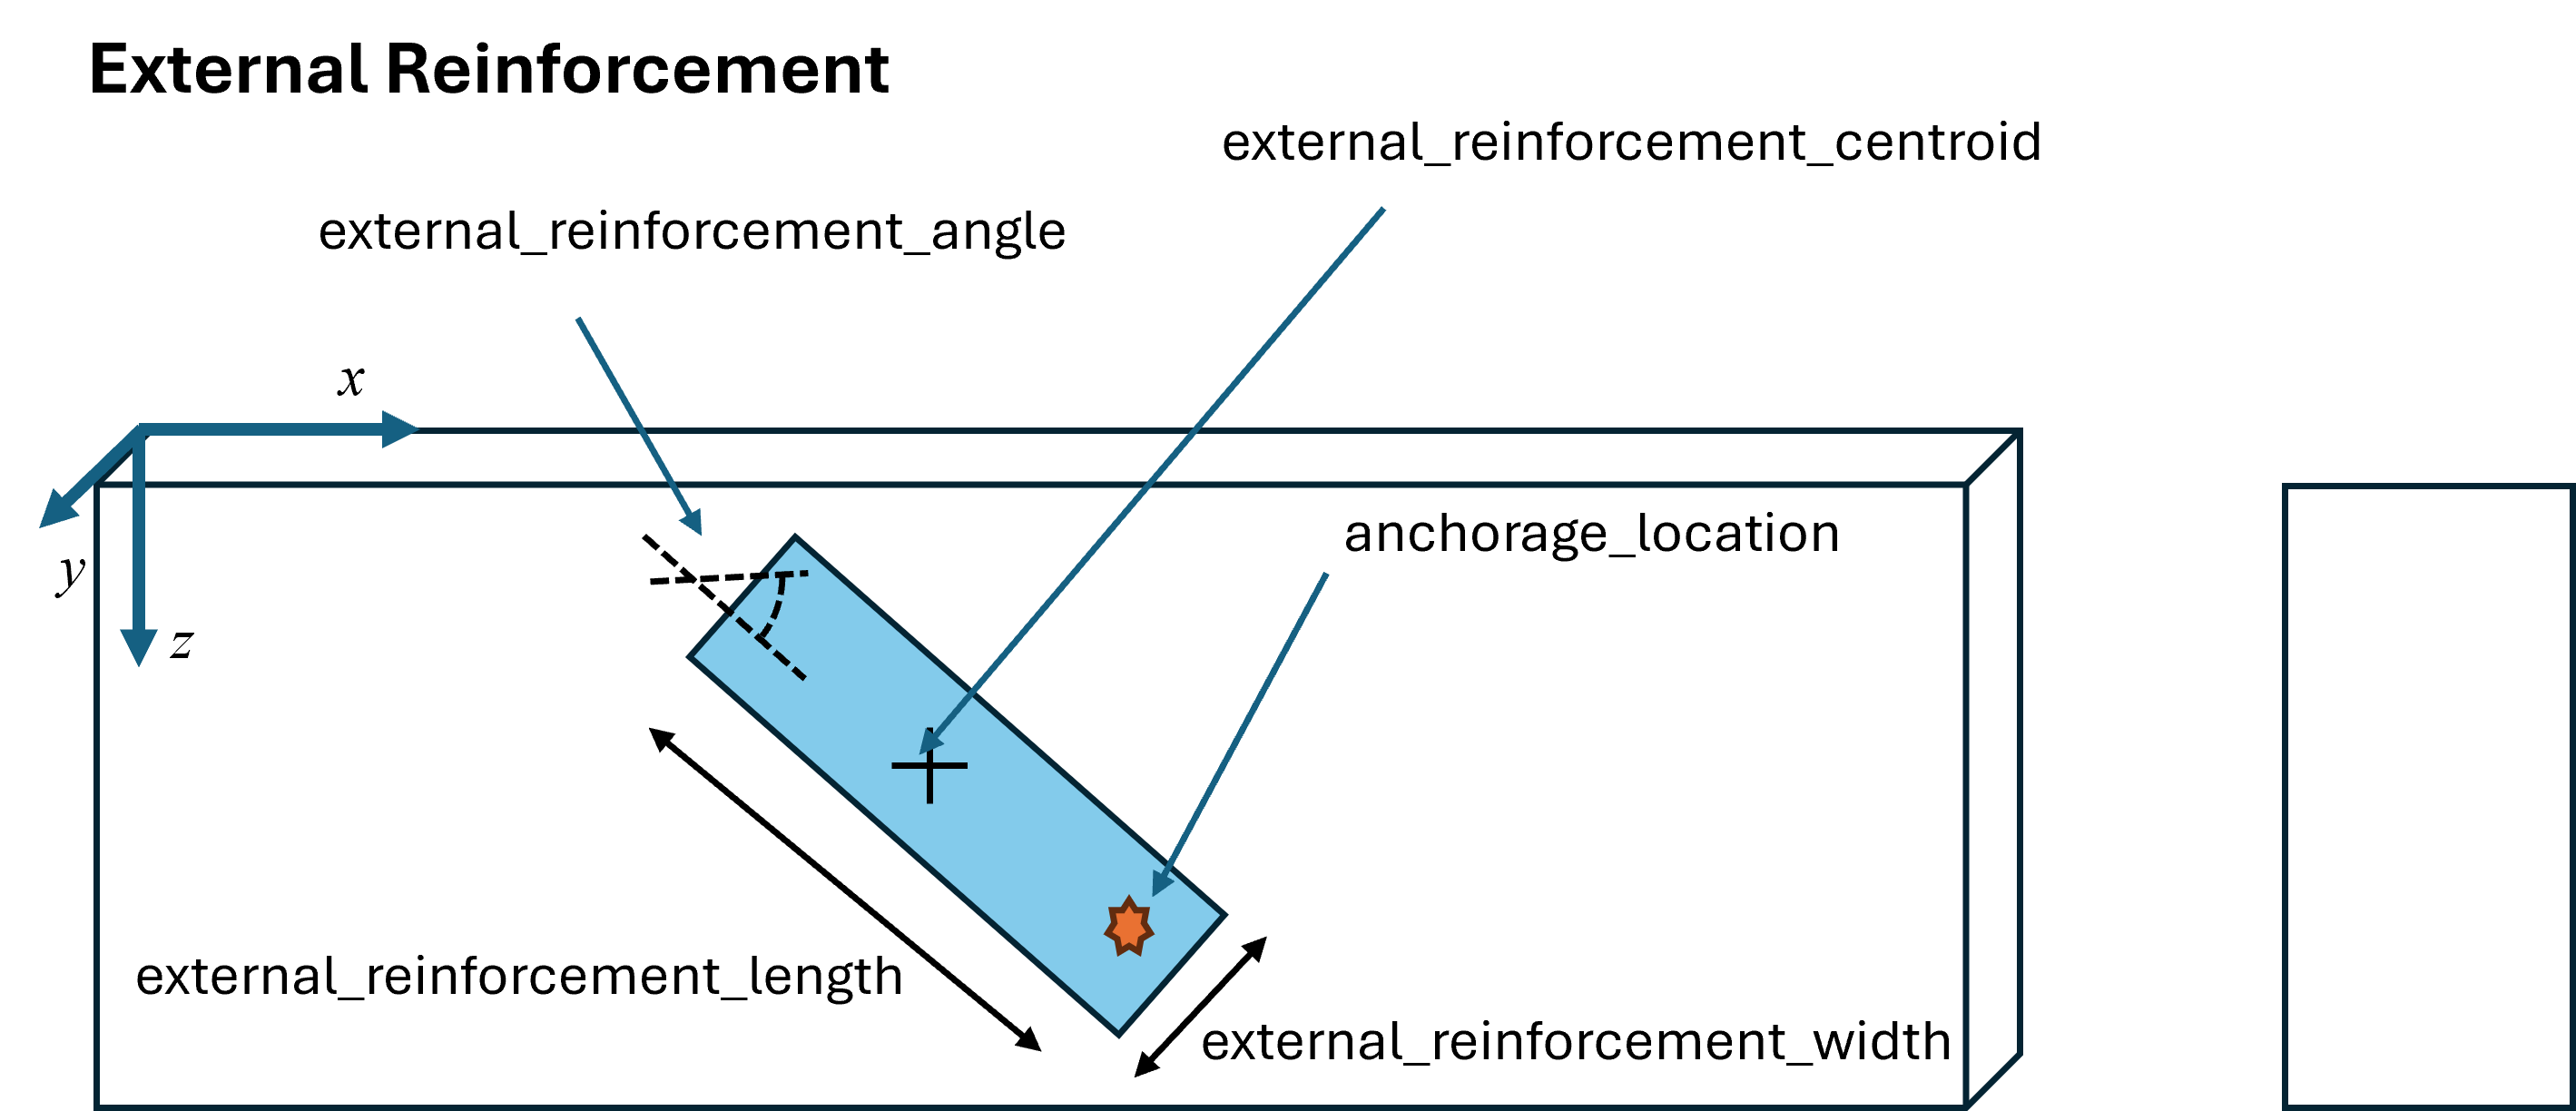
\includegraphics[width=\textwidth]{./figs/reinforcements/external_reinforcement.png}
    \caption{Parametrization of external reinforcement systems.}
    \label{fig:external_reinf}
\end{figure}

The parametrization is defined through the following parameters:

\begin{itemize}

    \item \texttt{reinforcement\_centroid\_x\_mm}: $x$ coordinate of the centroid of the external reinforcement system within the specimen coordinate system;

    \item \texttt{reinforcement\_centroid\_y\_mm}: $y$ coordinate of the centroid of the external reinforcement system within the specimen coordinate system;

    \item \texttt{reinforcement\_centroid\_z\_mm}: $z$ coordinate of the centroid of the external reinforcement system within the specimen coordinate system;

    \item \texttt{reinforcement\_width\_mm}: width of the external reinforcement region measured perpendicular to the principal reinforcement direction;

    \item \texttt{reinforcement\_length\_mm}: length of the external reinforcement region measured along the principal reinforcement direction;

    \item \texttt{reinforcement\_thickness\_mm}: thickness of the external reinforcement system;

    \item \texttt{reinforcement\_angle\_deg}: orientation angle of the external reinforcement measured relative to the reference structural axis shown in Fig.~\ref{fig:external_reinf};

    \item \texttt{anchorage\_size\_mm}: characteristic anchorage dimension or diameter;

    \item \texttt{anchorage\_location\_x\_mm}: $x$ coordinate of the anchorage location;

    \item \texttt{anchorage\_location\_y\_mm}: $y$ coordinate of the anchorage location;

    \item \texttt{anchorage\_location\_z\_mm}: $z$ coordinate of the anchorage location;

\end{itemize}

The reinforcement centroid coordinates define the global position of the external reinforcement system within the specimen coordinate system. The parameters \texttt{reinforcement\_length\_mm}, \texttt{reinforcement\_width\_mm}, and \texttt{reinforcement\_thickness\_mm} define the overall dimensions of the reinforcement region, while \texttt{reinforcement\_angle\_deg} defines its orientation relative to the structural member axes.

The adhesive-related parameters define the main mechanical characteristics of the bonding layer between the external reinforcement and the structural substrate. The anchorage-related parameters are optional and provide a simplified representation of supplemental anchorage systems used to improve force transfer or delay debonding failure.

When the current parametrization is insufficient to represent complex externally bonded reinforcement systems, contributors are encouraged to supplement the database entry with additional drawings, CAD files, annotated figures, photographs, laminate stacking descriptions, fiber-orientation specifications, or auxiliary documentation describing the reinforcement configuration in greater detail.

\newpage
\section{Test Geometry Parametrization Library}
The Test Geometry Parametrization Library defines the standardized parametric representations used to describe the geometry of experimental test setups throughout the database. Its primary purpose is to capture the geometric characteristics of the loading and boundary-condition configuration that are required for correct interpretation, comparison, and computational reproduction of experimental results. In many experimental tests, the interpretation of measured quantities depends not only on the specimen geometry, but also on the geometry of the test setup itself. For example, in modulus-of-rupture tests, the bending span is required, together with the specimen geometry, to compute the tensile strength from the measured peak load. Similarly, support spacing, loading-point locations, and other geometric descriptors may directly influence stress distributions, boundary conditions, failure mechanisms, and measured responses. The library therefore provides standardized parameter definitions and geometric descriptors for common experimental setups such as three-point bending, four-point bending, direct tension, compression, shear, pullout, torsion, and other test configurations. 


\subsection{\texttt{three\_point\_bending\_test}}
The \texttt{three\_point\_bending\_test}  parametrization defines the geometry of a three-point bending test setup through the following parameter (see Fig.~\ref{fig:3pbt}):

\begin{itemize}
    \item \texttt{bending\_span}: center-to-center distance between the two supports in the bending test configuration. The bending span defines the effective loaded span of the specimen and is a fundamental parameter for computing flexural stresses, modulus of rupture, stiffness, fracture energy, and other derived bending quantities.
\end{itemize}

\begin{figure}[htbp]
    \centering
    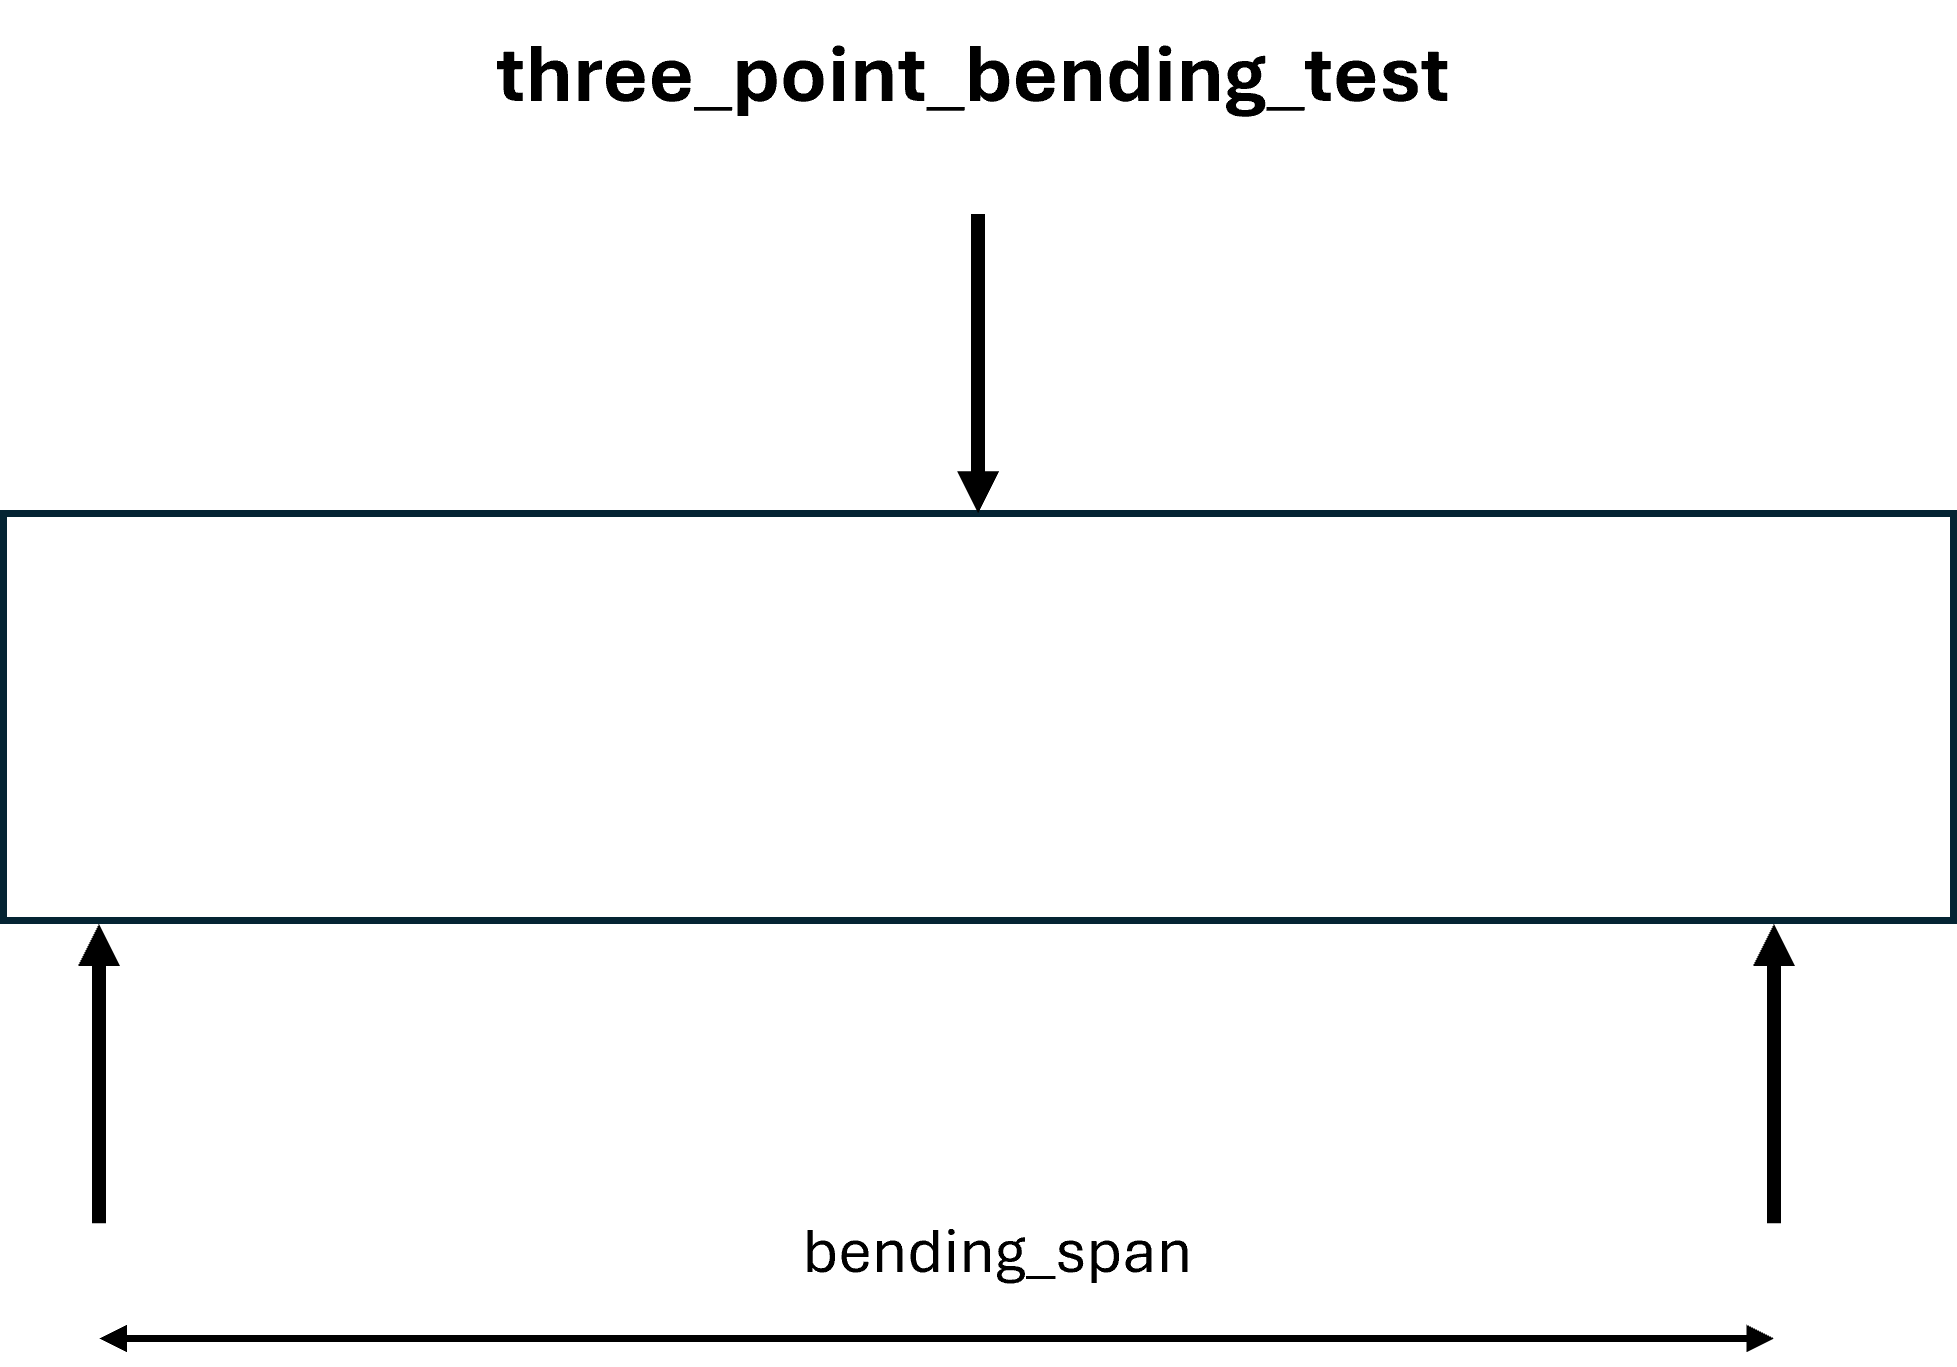
\includegraphics[width=0.4\textwidth]{./figs/tests/3pbt.png}
    \caption{Parametrization of external reinforcement systems.}
    \label{fig:3pbt}
\end{figure}

\subsection{\texttt{four\_point\_bending\_test} and \texttt{modulus\_of\_rupture\_test}}

The \texttt{four\_point\_bending\_test} (also applies to \texttt{modulus\_of\_rupture.text})  parametrization defines the geometry of a four-point bending test setup through the following parameters (see Fig.~\ref{fig:4pbt}):

\begin{itemize}
    \item \texttt{bending\_span}: center-to-center distance between the two supports in the bending test configuration. The bending span defines the effective loaded span of the specimen and is a fundamental parameter for computing flexural stresses, stiffness, fracture energy, and other derived bending quantities.
    
    \item \texttt{shear\_span}: distance between a support and the nearest loading point measured along the longitudinal axis of the specimen. In symmetric four-point bending configurations, the shear span is equal to one-half of the difference between the bending span and the loading span. The shear span strongly influences the internal shear-force distribution, cracking patterns, failure mode, and the relative contribution of flexural and shear mechanisms.
\end{itemize}

\begin{figure}[htbp]
    \centering
    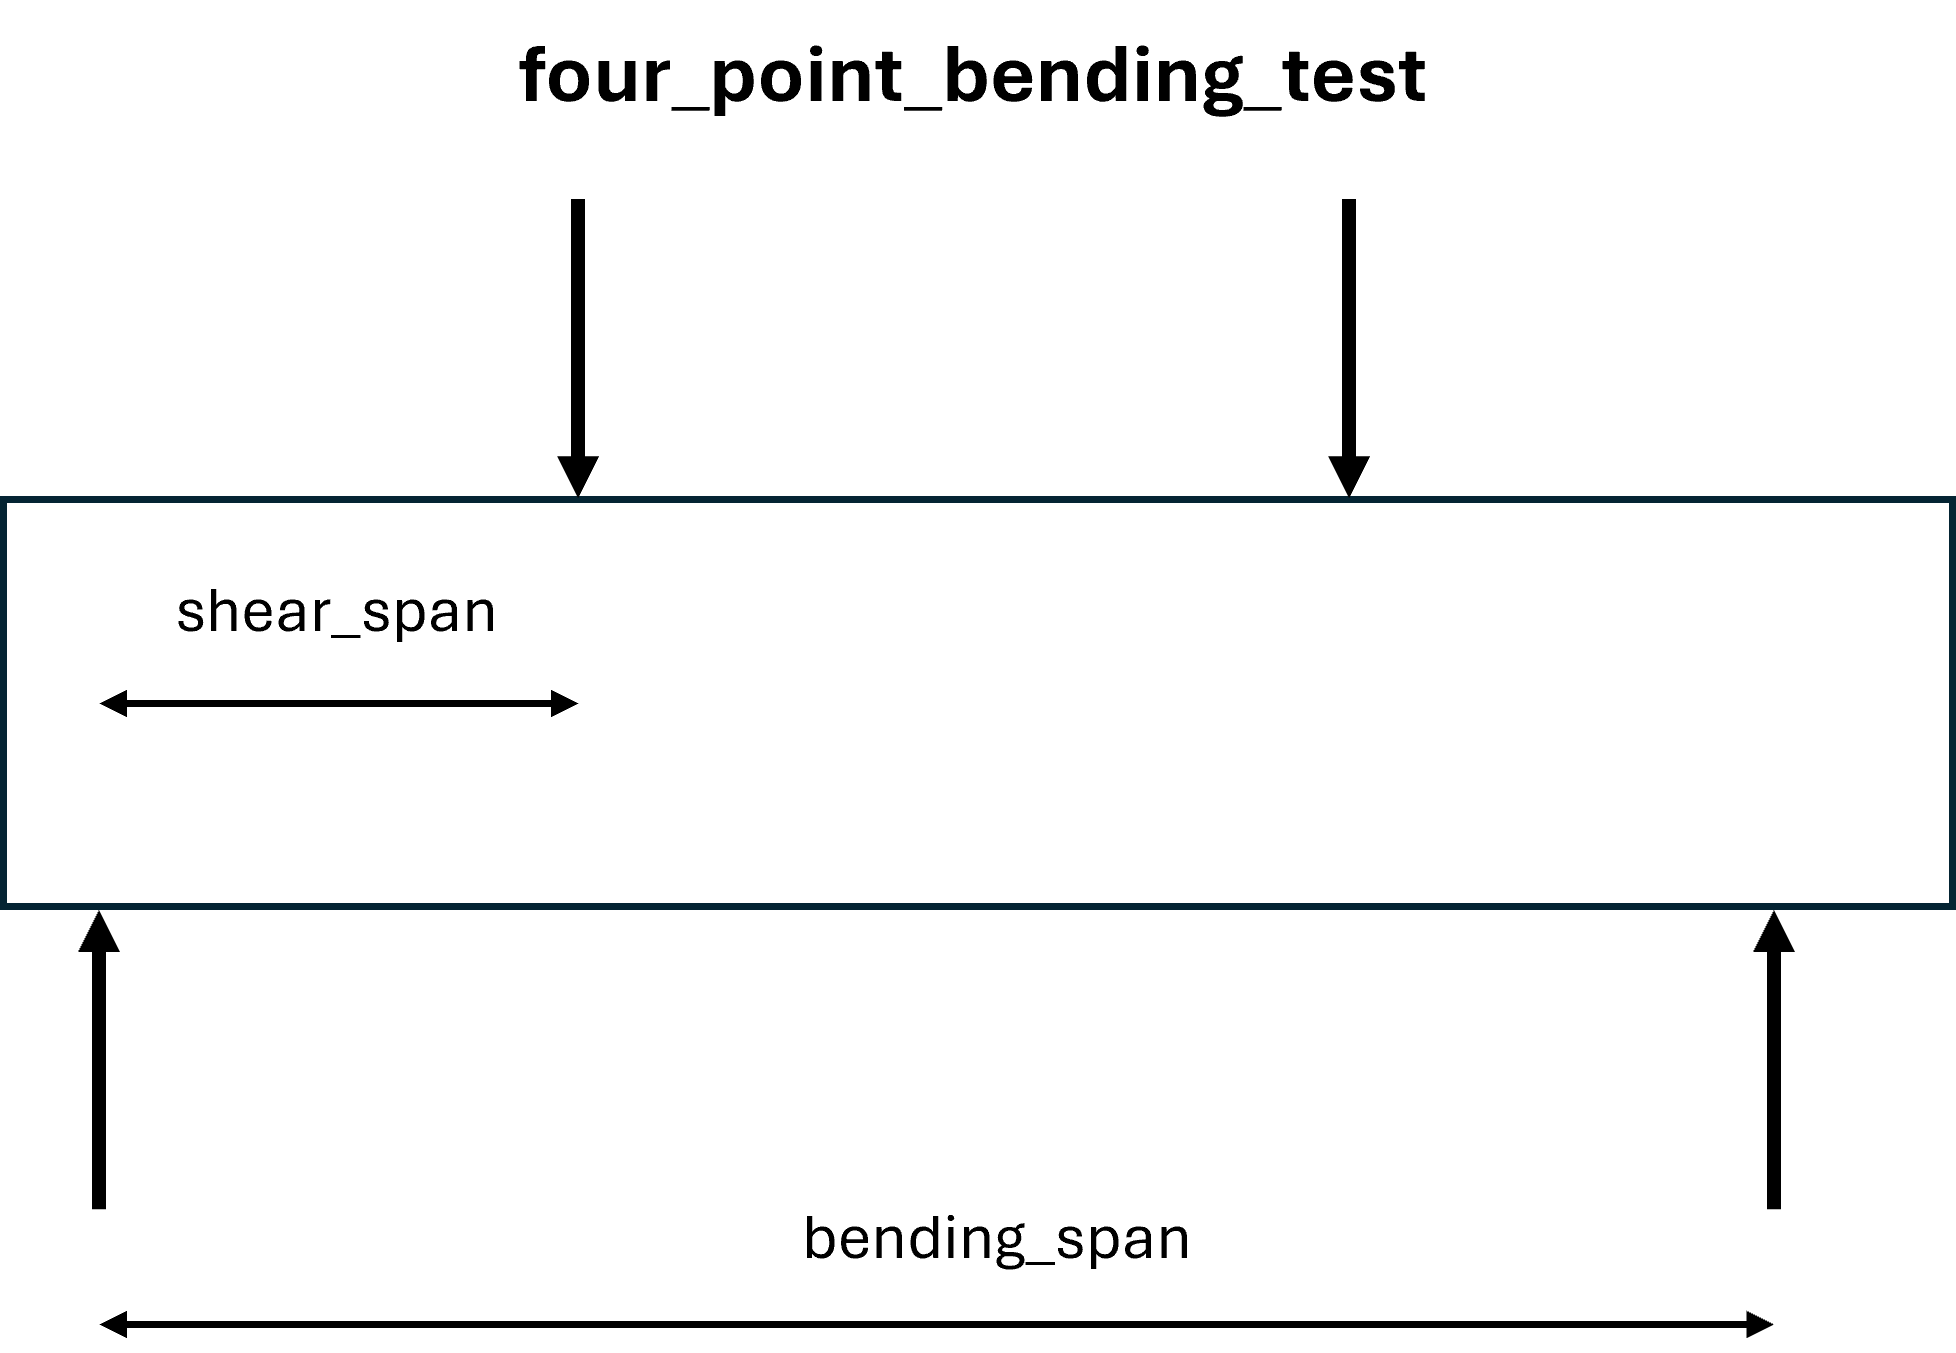
\includegraphics[width=0.4\textwidth]{./figs/tests/4pbt.png}
    \caption{Parametrization of the four-point bending test setup.}
    \label{fig:4pbt}
\end{figure}


\subsection{\texttt{axial\_test}}

The \texttt{axial\_test} parametrization defines the geometry of an axial loading test in which the applied load is offset from the centroidal axis of the specimen, thereby introducing combined axial force and bending effects (see Fig.~\ref{fig:axial_test_eccentricity}).

\begin{itemize}
    \item \texttt{eccentricity}: perpendicular distance between the line of action of the applied axial load and the centroidal axis of the specimen cross section. The eccentricity governs the magnitude of the induced bending moment.
\end{itemize}

\begin{figure}[htbp]
    \centering
    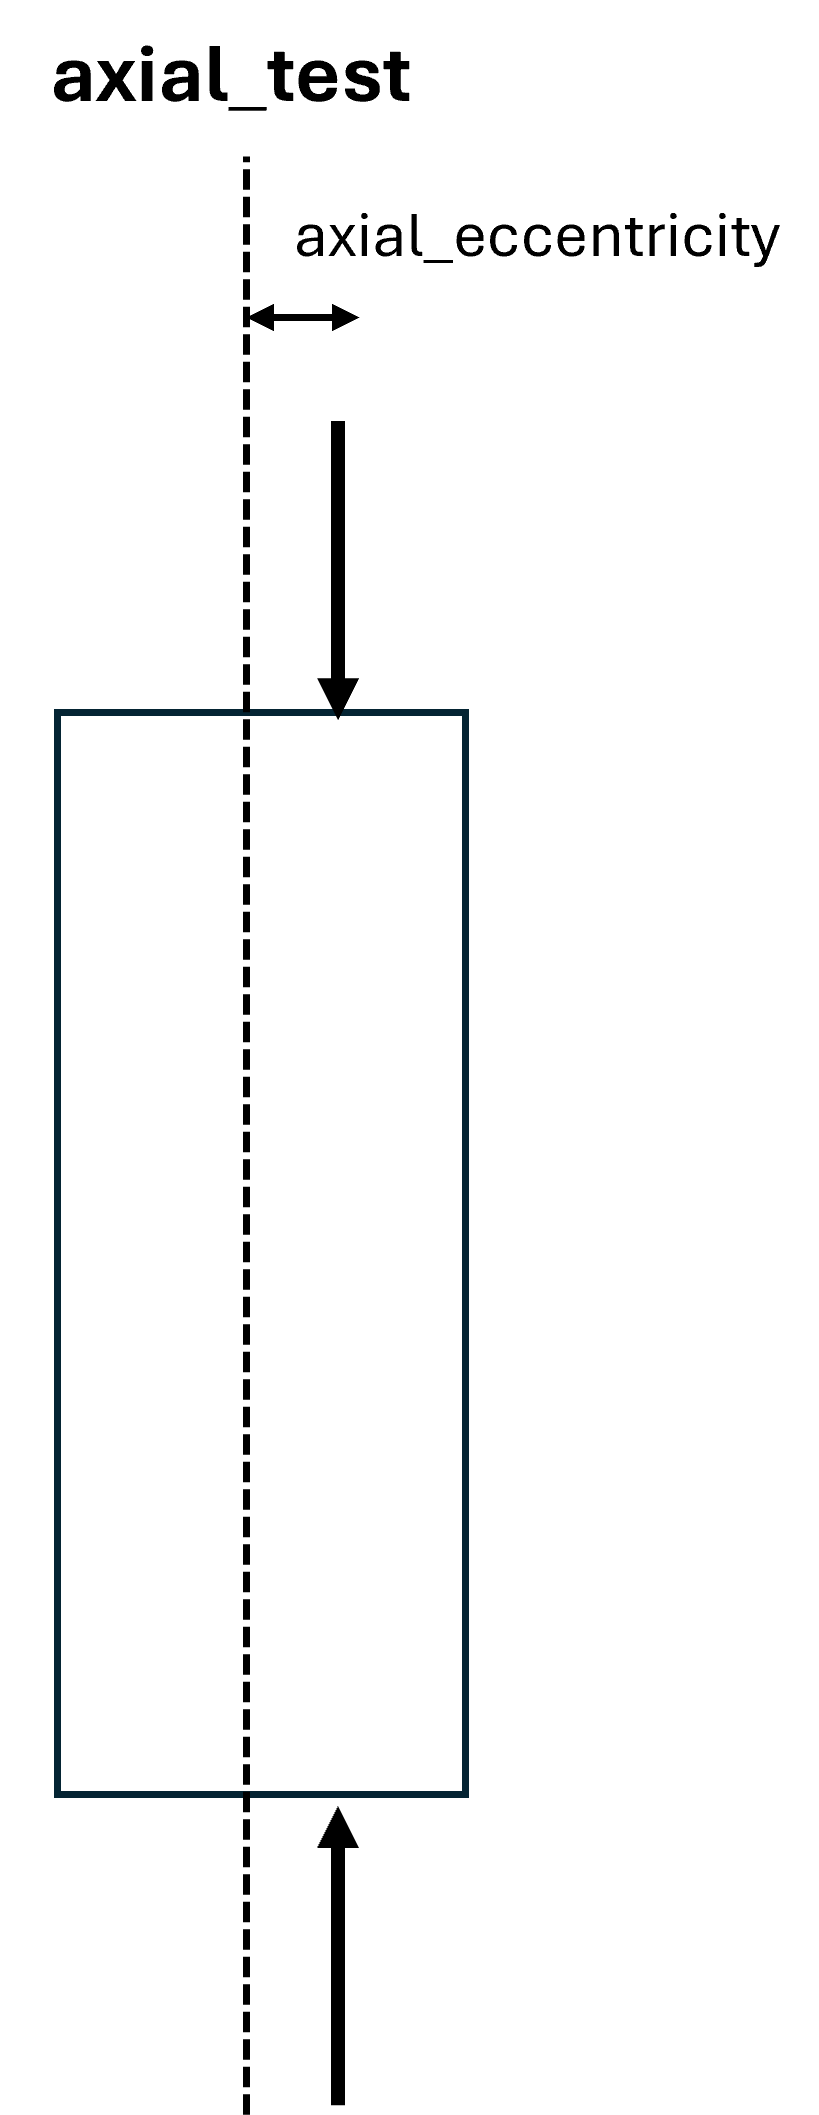
\includegraphics[width=0.15\textwidth]{./figs/tests/axial_test.png}
    \caption{Parametrization of the axial loading test with eccentricity.}
    \label{fig:axial_test_eccentricity}
\end{figure}


\newpage

\section{Devices \& Supports Parametrization Library}


The Devices \& Supports Parametrization Library defines the standardized parametric representations used to describe the experimental devices, supports, fixtures, loading components, and instrumentation systems associated with experimental tests throughout the database. Its primary purpose is to provide structured machine-readable descriptions of the key characteristics of experimental components that may influence the interpretation, accuracy, reproducibility, and computational representation of test results. The library will include standardized parameter definitions for a broad range of devices and supports such as LVDTs, extensometers, CMOD gauges, load cells, actuators, loading platens, rollers, hinges, soft pads, clamps, cameras, and DIC systems. Depending on the device type, the parametrization may include geometric descriptors, spatial locations, orientations, measurement directions, gage lengths, support dimensions, platen sizes, load-cell capacities, sensor resolutions, sampling frequencies, stiffness properties, constitutive properties, and other relevant parameters required to characterize the experimental setup. Additional parameters and more advanced parametrization may be incorporated in future extensions of the devices and supports parametrization library distributed through the accompanying \texttt{devices\_and\_supports\_library.json} file ({\emph{under development}).

\subsection{\texttt{pad\_support}}

The \texttt{pad\_support} parametrization defines deformable pad supports used to model compliant boundary conditions in experimental setups (Fig.~\ref{fig:pad_support}). The parametrization is intended to represent elastomeric pads, neoprene supports, soft interface layers, wooden strips, or other deformable support materials commonly adopted to reduce stress concentrations, accommodate local rotations, or provide distributed contact conditions between the specimen and the supporting structure.

All coordinates and dimensions are defined within the right-handed Cartesian coordinate system associated with the corresponding specimen geometry. The support location is specified through the coordinates \texttt{x\_location\_mm}, \texttt{y\_location\_mm}, and \texttt{z\_location\_mm}, while the parameter \texttt{orientation} defines the principal support direction relative to the specimen coordinate system.

The deformable pad is defined through the following parameters:

\begin{itemize}
    \item \texttt{depth}: pad dimension measured along the axis defined by the \texttt{orientation} parameter and orthogonal to the contact surface;
    
    \item \texttt{thickness}: pad thickness measured in-plane to the contact surface;
    
    \item \texttt{length}: pad dimension measured in-plane to the contact surface;
    
    \item \texttt{material}: optional description of the pad material;
    
    \item \texttt{elastic\_modulus}: elastic modulus of the pad material;
    
    \item \texttt{yielding\_stress}: optional yield stress of the pad material;
    
    \item \texttt{stress\_vs\_strain\_curve}: optional embedded constitutive stress-strain response of the pad material represented through pairs of strain and stress values.
\end{itemize}

Additional parameters and more advanced support descriptions may be incorporated in future extensions of the devices and supports parametrization library distributed through the accompanying \texttt{devices\_and\_supports\_library.json} file.

\begin{figure}[htbp]
    \centering
    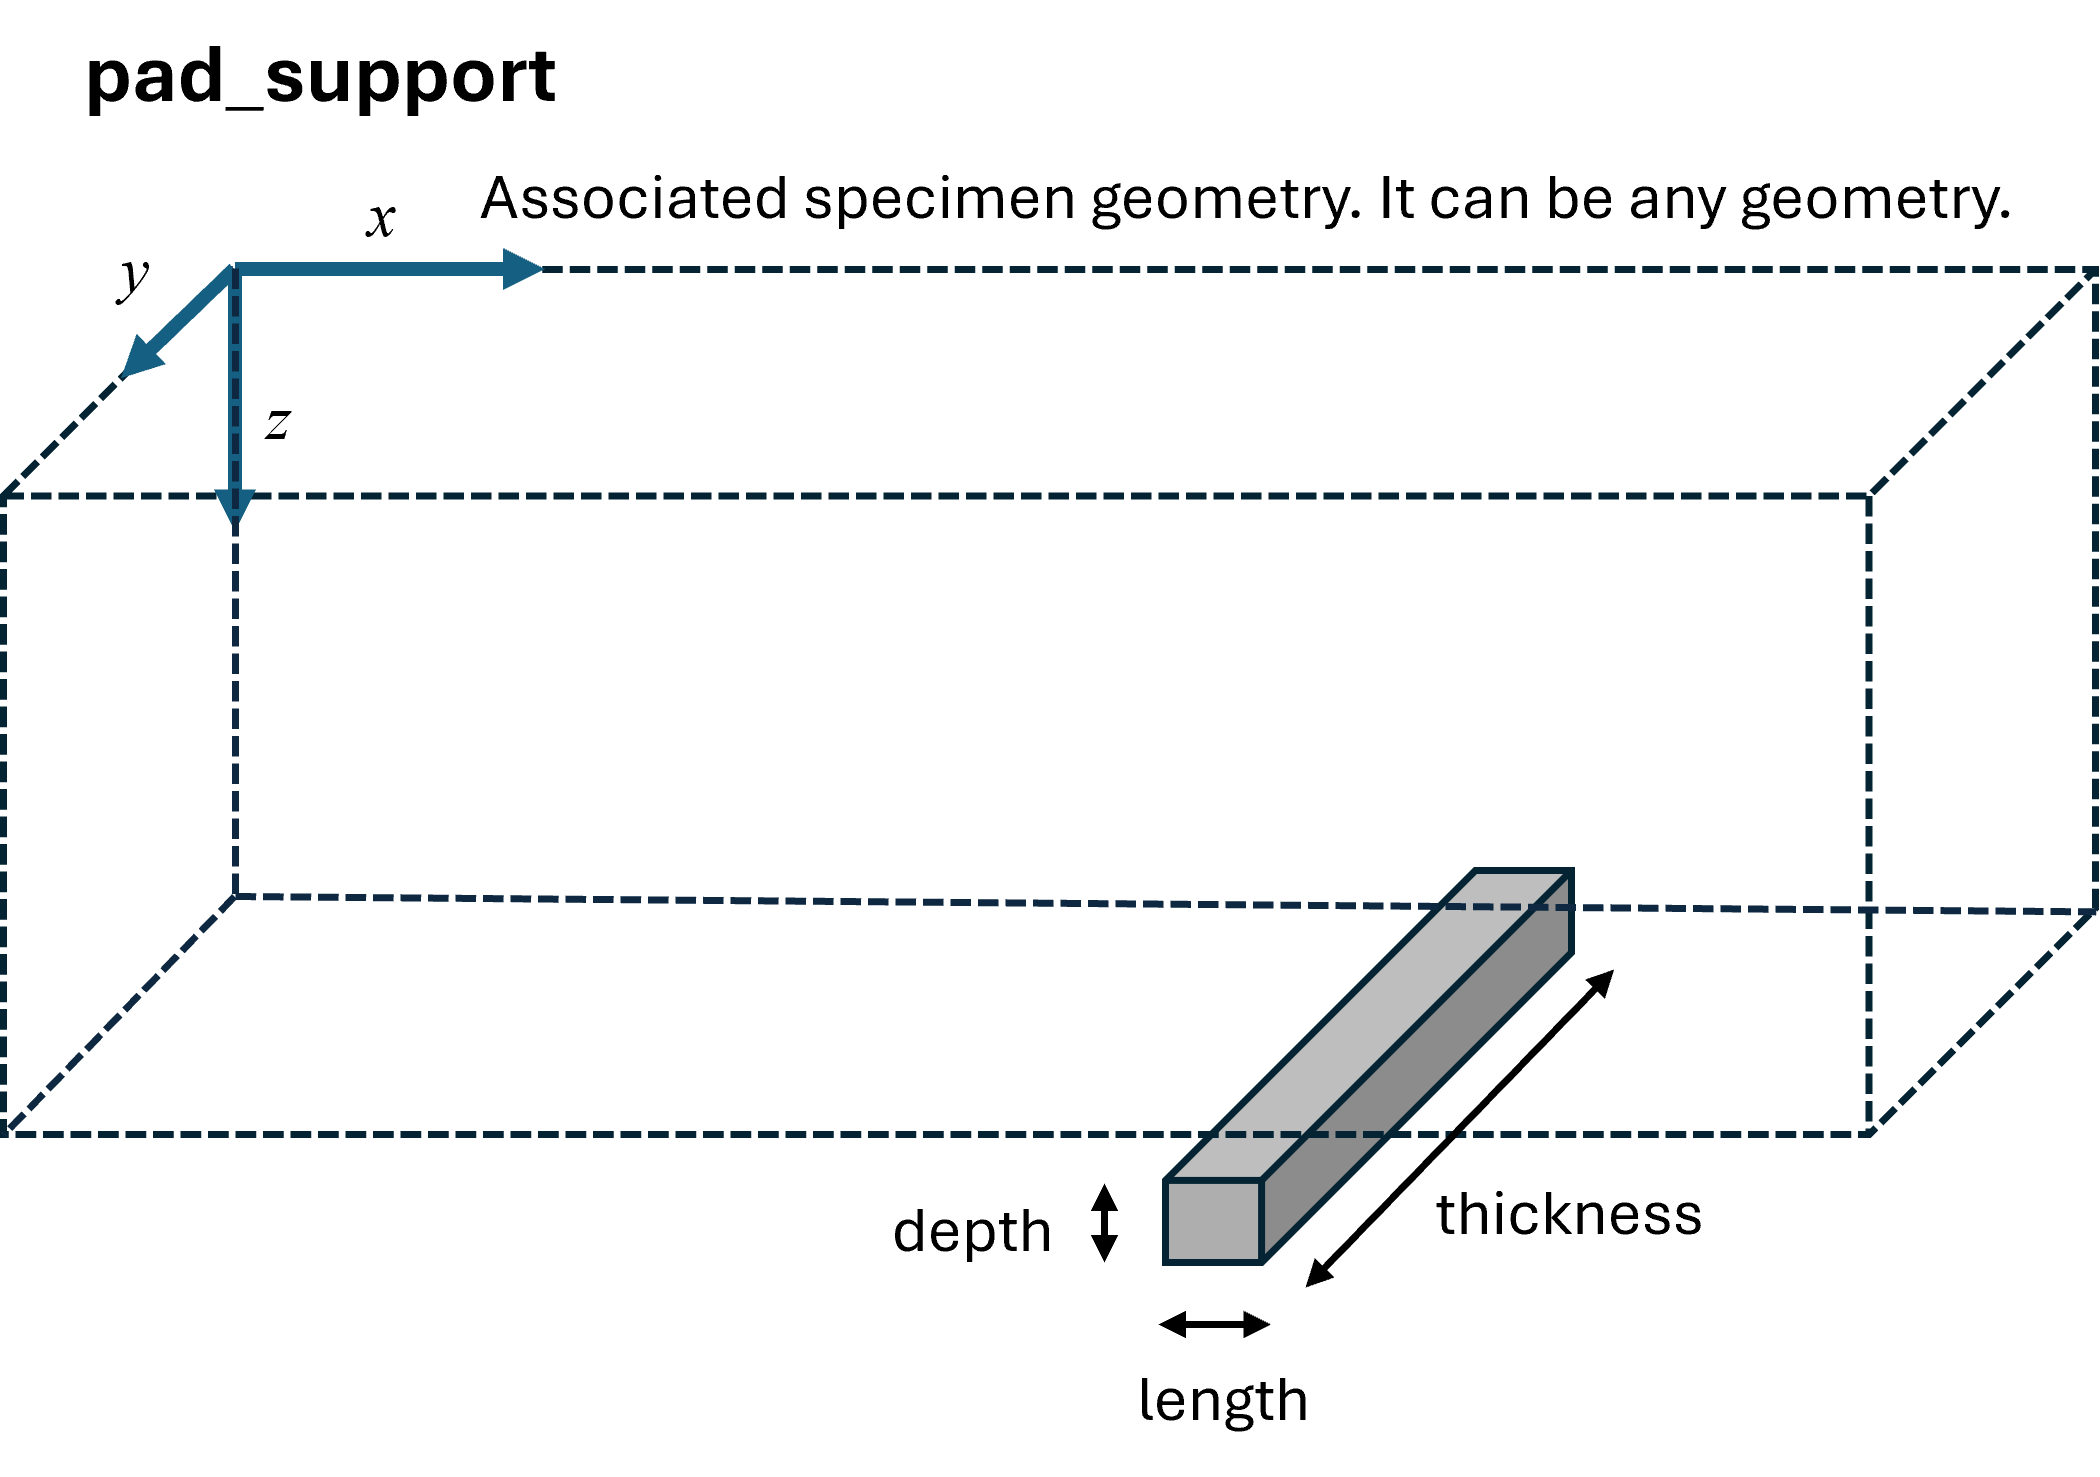
\includegraphics[width=0.4\textwidth]{./figs/supports/pad_support.png}
    \caption{Parametrization of deformable pad supports.}
    \label{fig:pad_support}
\end{figure}


\subsection{\texttt{roller\_support}}

The \texttt{roller\_support} parametrization defines cylindrical roller supports used to constrain only deflection in the direction of the sliding plane (Fig.~\ref{fig:roller_support}). Roller supports are commonly adopted in flexural, fracture, and structural testing to provide translational freedom along the sliding plane and minimizing restraint forces and parasitic moments at the specimen boundaries.

All coordinates and dimensions are defined within the right-handed Cartesian coordinate system associated with the corresponding specimen geometry. The support location is specified through the coordinates \texttt{x\_location\_mm}, \texttt{y\_location\_mm}, and \texttt{z\_location\_mm}, while the parameter \texttt{orientation} defines the principal axis of the cylindrical roller relative to the specimen coordinate system.

The cylindrical roller support is defined through the following parameters:

\begin{itemize}
    \item \texttt{length}: total roller length measured along the roller axis defined by the \texttt{orientation} parameter;
    
    \item \texttt{diameter}: diameter of the cylindrical roller;
    
    \item \texttt{material}: optional description of the roller material;
    
    \item \texttt{elastic\_modulus}: optional elastic modulus of the roller material;
    
    \item \texttt{yielding\_stress}: optional yield stress of the roller material;
    
    \item \texttt{surface\_roughness}: optional characteristic surface roughness of the roller contact surface.
\end{itemize}



\begin{figure}[htbp]
    \centering
    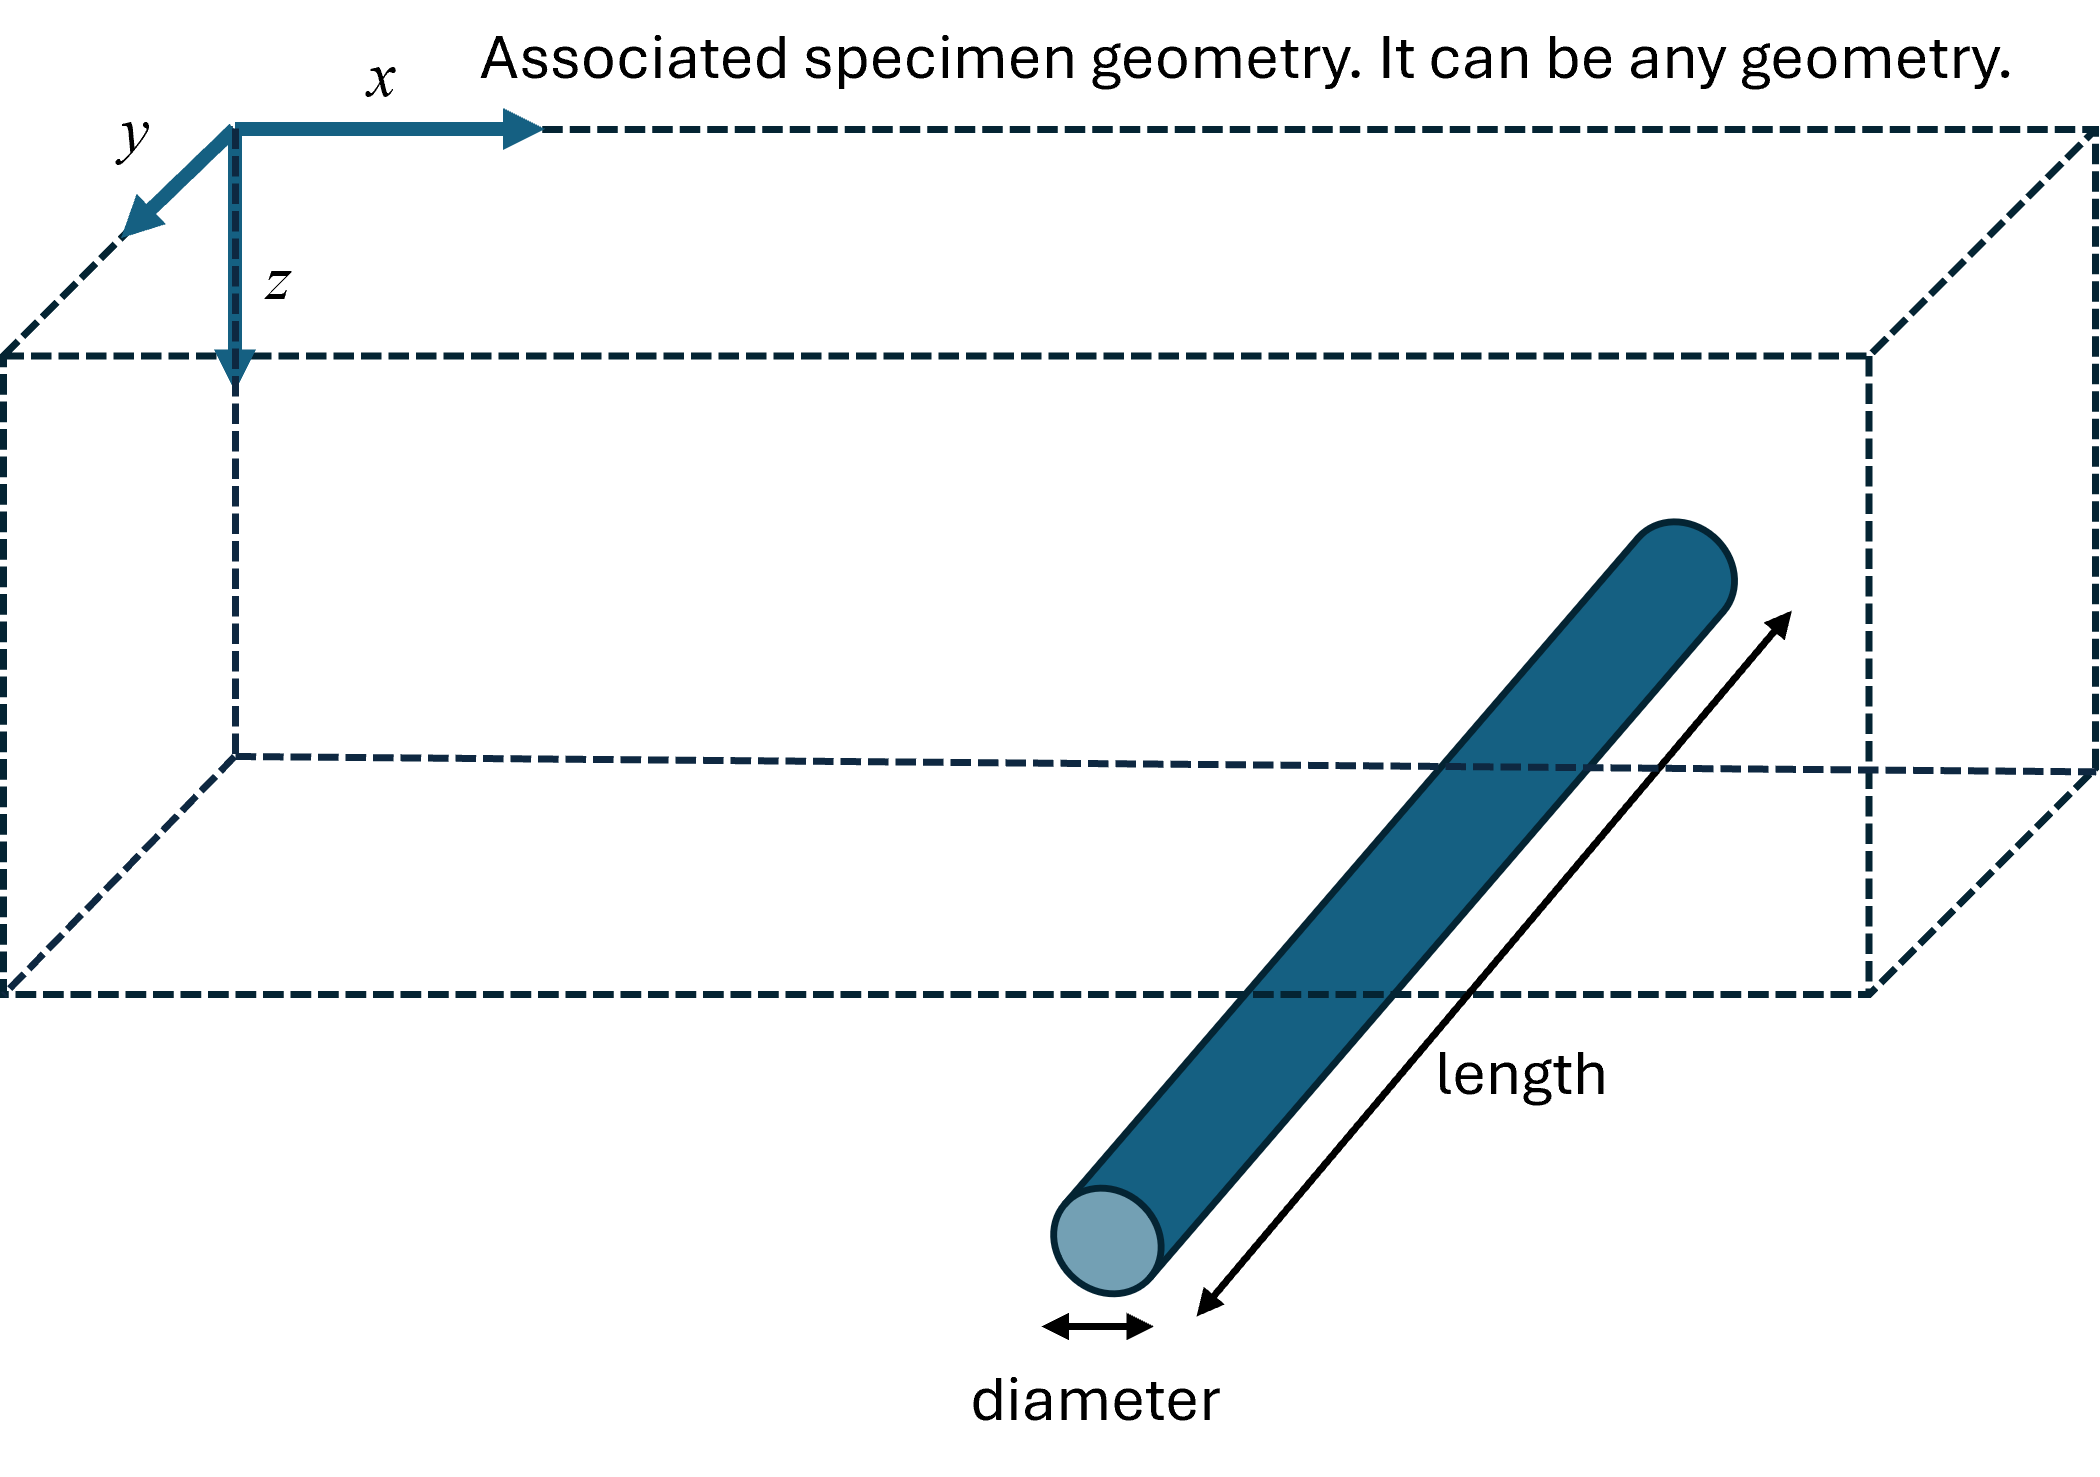
\includegraphics[width=0.35\textwidth]{./figs/supports/roller_support.png}
    \caption{Parametrization of cylindrical roller supports.}
    \label{fig:roller_support}
\end{figure}




\newpage

\chapter{Controlled Vocabulary Reference}
\label{Part:Vocab}
This part summarizes the controlled vocabularies adopted throughout the database. The controlled vocabulary entries include both the standardized fields used in the data-collection spreadsheet tabs and the predefined lists contained in the \texttt{Vocab} tab, which define the drop-down menus used across the various spreadsheet tabs. These vocabularies are further complemented by accompanying machine-readable JSON vocabulary definition files (\emph{currently under development}).

\begin{itemize}
%
   \item \hyperref[vocab:identifiers]{\texttt{identifiers}}
%
   \item \hyperref[vocab:literature_source_tab_fields]{\texttt{literature\_sources\_tab}}
   \begin{itemize}
           \item \hyperref[vocab:source_type_list]{\texttt{source\_type\_list}}
   \end{itemize}
%
   \item \hyperref[vocab:material_batch_tab_fields]{\texttt{material\_batches\_tab}}
   \begin{itemize}
        \item \hyperref[vocab:material_class_list]{\texttt{material\_class\_list}}
        \item \hyperref[vocab:cement_type_list]{\texttt{cement\_type\_list}}
        \item \hyperref[vocab:aggregate_type_list]{\texttt{aggregate\_type\_list}}
        \item \hyperref[vocab:superplasticizer_type_list]{\texttt{superplasticizer\_type\_list}}
        \item \hyperref[vocab:water_reducer_type_list]{\texttt{water\_reducer\_type\_list}}
        \item \hyperref[vocab:air_entrainment_type_list]{\texttt{air\_entrainment\_type\_list}}
        \item \hyperref[vocab:rheology_modifier_type_list]{\texttt{rheology\_modifier\_type\_list}}
        \item \hyperref[vocab:hydration_accelerator_type_list]{\texttt{hydration\_accelerator\_type\_list}}
%        \item \hyperref[vocab:aggregate_type_list]{\texttt{aggregate\_type\_list}}
        \item \hyperref[vocab:fiber_type_list]{\texttt{fiber\_type\_list}}
   \end{itemize}
%
   \item \hyperref[vocab:reinforcement_materials_tab]{\texttt{reinforcement\_materials\_tab}}
   \begin{itemize}
        \item \hyperref[vocab:reinforcement_material_types_list]{\texttt{reinforcement\_material\_type\_list}}   
   \end{itemize}
%
   \item \hyperref[vocab:geometry_fields_tab]{\texttt{geometries\_tab}}
   \begin{itemize}
        \item \hyperref[vocab:specimen_geometry_type_list]{\texttt{specimen\_geometry\_type\_list}}
   \end{itemize}
% 
   \item \hyperref[vocab:reinforcement_fields_tab]{\texttt{reinforcement\_components\_tab}}
   \begin{itemize}
        \item \hyperref[vocab:reinforcement_material_types_list]{\texttt{reinforcement\_material\_type\_list}}   
        \item \hyperref[vocab:reinforcement_type_list]{\texttt{reinforcement\_type\_list}}
        \item \hyperref[vocab:bar_designation_list]{\texttt{bar\_designation\_list}}
        \item \hyperref[vocab:adhesive_type_list]{\texttt{adhesive\_type\_list}}
        \item \hyperref[vocab:anchorage_type_list]{\texttt{anchorage\_type\_list}}
   \end{itemize}
% 
   \item \hyperref[vocab:reinforcement_layouts_fields_tab]{\texttt{reinforcement\_layouts\_tab}}
%
   \item \hyperref[vocab:specimen_fields_tab]{\texttt{specimens\_tab}}
   \begin{itemize}
        \item \hyperref[vocab:structural_form_type_list]{\texttt{structural\_form\_type\_list}}
   \end{itemize}
%   
   \item \hyperref[vocab:test_fields_tab]{\texttt{test\_fields\_tab}}
   \begin{itemize}
      \item \hyperref[vocab:test_type_list]{\texttt{test\_type\_list}}
      \item \hyperref[vocab:observed_mechanisms_list]{\texttt{observed\_mechanisms\_list}}
      \item \hyperref[vocab:curing_conditions_list]{\texttt{curing\_conditions\_list}}
      \item \hyperref[vocab:boundary_conditions_list]{\texttt{hygral\_boundary\_conditions\_list}}      
      \item \hyperref[vocab:boundary_conditions_list]{\texttt{thermal\_boundary\_conditions\_list}}
    \end{itemize}
%
   \item \hyperref[vocab:devices_and_supports_fields_tab]{\texttt{devices\_and\_supports\_fields\_tab}}
   \begin{itemize}
         \item \hyperref[vocab:devices_and_supports_list]{\texttt{devices\_and\_supports\_list}}
    \end{itemize}
%
   \item \hyperref[vocab:loading_history_fields_tab]{\texttt{loading\_history\_fields\_tab}}
   \begin{itemize}
         \item \hyperref[vocab:loading_modes_list]{\texttt{loading\_modes\_list}}
         \item \hyperref[vocab:loading_control_variable_list]{\texttt{loading\_control\_variable\_list}}
    \end{itemize}
%
   \item \hyperref[vocab:data_fields_tab]{\texttt{data\_fields\_tab}}
   \begin{itemize}
         \item \hyperref[vocab:extraction_methods_list]{\texttt{extraction\_methods\_list}}
         \item \hyperref[vocab:data_types_list]{\texttt{data\_type\_list}}
         \item \hyperref[vocab:reported_quantity_list]{\texttt{quantity\_reported\_list}}
         \item \hyperref[vocab:quantity_reported_type_list]{\texttt{quantity\_reported\_type\_list}}
    \end{itemize}
\end{itemize}

\section{Identifiers}
\label{vocab:identifiers}
The following table defines the identifiers used in the database. The machine-readable definitions of these vocabulary entries are provided in \texttt{identifiers.json}. The database adopts standardized identifiers to uniquely define and reference the main entities contained in the hierarchical data structure. Each identifier follows a fixed alphanumeric format composed of a prefix indicating the entity type and a progressive numerical index. These identifiers are used throughout the spreadsheet, JSON files, validation schemas, and file organization structure.

\begin{longtable}{p{0.32\textwidth}p{0.12\textwidth}p{0.48\textwidth}}
\hline
\textbf{Identifier} & \textbf{Format} & \textbf{Definition} \\
\hline
\endfirsthead

\hline
\textbf{Identifier} & \textbf{Format} & \textbf{Definition} \\
\hline
\endhead

\texttt{source\_id} & \texttt{SRC0001} &
Unique identifier of a literature source, report, thesis, dataset, or experimental campaign representing the top-level entity in the database hierarchy. \\

\texttt{batch\_id} & \texttt{BAT0001} &
Unique identifier of a material mixture, material batch, or material system definition. \\

\texttt{reinforcement\_material\_id} & \texttt{RMT0001} &
Unique identifier of a reusable reinforcement material definition containing the material properties associated with reinforcement systems. \\

\texttt{geometry\_id} & \texttt{GEO0001} &
Unique identifier of a reusable specimen geometry definition based on the geometry parametrization library. \\

\texttt{printing\_id} & \texttt{PRI0001} &
Unique identifier of a reusable definition of additive manufacturing or printing process variables. \\

\texttt{reinforcement\_layout\_id} & \texttt{RFL0001} &
Unique identifier of a reusable reinforcement layout associated with a specimen geometry and composed of one or more reinforcement components. \\

\texttt{reinforcement\_component\_id} & \texttt{REF0001} &
Unique identifier of an individual reinforcement component, such as a rebar layer, stirrup set, tie set, or external reinforcement system, associated with a reinforcement layout. \\

\texttt{specimen\_id} & \texttt{SPC0001} &
Unique identifier of a physical specimen or specimen family defined by the combination of material batch, geometry, optional reinforcement layout, and optional printing variables. \\

\texttt{test\_id} & \texttt{TST0001} &
Unique identifier of an experimental test performed on a specimen. \\

\texttt{device\_id} & \texttt{DEV0001} &
Unique identifier of a support, actuator, sensor, fixture, instrumentation component, or measurement device associated with a test. \\

\texttt{loading\_id} & \texttt{LDG0001} &
Unique identifier of a loading protocol or loading history associated with a test and, when applicable, with a specific device. \\

\texttt{data\_id} & \texttt{DAT0001} &
Unique identifier of an experimental observation or dataset, including scalar quantities, curves, tables, images, videos, and multidimensional field data. \\

\hline
\end{longtable}

\section{Literature Source Tab Fields}
\label{vocab:literature_source_tab_fields}

The following table defines the fields used in the \texttt{literature\_sources} tab. The machine-readable definitions of these vocabulary entries are provided in \texttt{literature\_source\_tab\_fields.json}.

\begin{longtable}{p{0.26\textwidth}p{0.7\textwidth}}
\hline
\textbf{Field Name} & \textbf{Definition} \\
\hline
\endfirsthead

\hline
\textbf{Field Name} & \textbf{Definition} \\
\hline
\endhead

\texttt{source\_type} &
Classification of the source document type. \\

\texttt{peer\_reviewed} &
Boolean field indicating whether the source underwent formal peer review prior to publication. \\

\texttt{title} &
Full title of the publication. \\

\texttt{authors} &
List of authors associated with the source document. \\

\texttt{year} &
Year of publication or public release of the source document. \\

\texttt{journal\_or\_publisher} &
Name of the journal, conference proceedings, publishing organization, institution, or publisher associated with the source. \\

\texttt{volume} &
Journal or proceedings volume number when applicable. \\

\texttt{issue} &
Journal or proceedings issue number when applicable. \\

\texttt{pages} &
Page range associated with the source document when applicable. \\

\texttt{doi} &
Digital Object Identifier associated with the source document. \\

\texttt{url} &
Web address or online repository link associated with the source document or dataset. \\

\texttt{institution} &
Institution, laboratory, university, company, agency, or organization associated with the source document or experimental program. \\

\hline
\end{longtable}

\subsection{Literature Source Types}
\label{vocab:source_type_list}

The following table defines the controlled vocabulary for the \texttt{source\_type} field used in the \texttt{literature\_sources} tab. The machine-readable definitions of these vocabulary entries are provided in \texttt{source\_types.json}. 

\begin{longtable}{p{0.24\textwidth}p{0.78\textwidth}}
\hline
\textbf{Term} & \textbf{Definition} \\
\hline
\endfirsthead

\hline
\textbf{Term} & \textbf{Definition} \\
\hline
\endhead

\texttt{book\_chapter} &
A chapter published within an edited book or proceedings volume. \\

\texttt{conference\_paper} &
A paper published in conference proceedings or presented at a scientific or engineering conference. \\

\texttt{dataset} &
A standalone curated dataset, database, or data repository entry. \\

\texttt{journal\_article} &
An article published in a scientific, technical, or professional journal. \\

\texttt{phd\_thesis} &
A doctoral dissertation or PhD thesis submitted as part of a doctoral degree program. \\

\texttt{report} &
A technical, institutional, governmental, industrial, or research report. \\

\texttt{other} &
A source type that does not fall within the predefined categories. \\

\hline
\end{longtable}


\section{Material Batch Tab Fields}
\label{vocab:material_batch_tab_fields}

The following table defines the fields used in the \texttt{material\_batches} tab. The machine-readable definitions of these vocabulary entries are provided in \texttt{material\_batches\_tab\_fields.json}

\begin{longtable}{p{0.42\textwidth}p{0.54\textwidth}}
%\caption{Material batch fields.}
%\label{tab:material_batch_fields}\\
\hline
\textbf{Field Name} & \textbf{Definition} \\
\hline
\endfirsthead

\hline
\textbf{Field Name} & \textbf{Definition} \\
\hline
\endhead

\texttt{mixing\_protocol\_file\_name} &
File name associated with the documented material mixing procedure or batching protocol. \\

\texttt{batch\_label} &
Original batch designation or identifier used in the source documentation or laboratory records. \\

\texttt{material\_class} &
General material classification associated with the batch. \\

\texttt{cement\_type} &
Type or designation of cement used in the mixture. \\

\texttt{printable} &
Boolean field indicating whether the mixture was designed for additive manufacturing or extrusion-based placement processes. \\

\texttt{self\_consolidating} &
Boolean field indicating whether the mixture qualifies as self-consolidating concrete or mortar. \\

\texttt{cement\_content\_kg\_m3} &
Mass of cement per cubic meter of material. \\

\texttt{water\_binder\_ratio} &
Ratio between total water content and total binder content by mass. \\

\texttt{silica\_fume\_content\_kg\_m3} &
Mass of silica fume per cubic meter of material. \\

\texttt{fly\_ash\_content\_kg\_m3} &
Mass of fly ash per cubic meter of material. \\

\texttt{fly\_ash\_class} &
Classification or designation of fly ash used in the mixture. \\

\texttt{slag\_content\_kg\_m3} &
Mass of slag or ground granulated blast furnace slag per cubic meter of material. \\

\texttt{fine\_aggregate\_content\_kg\_m3} &
Mass of fine aggregate per cubic meter of material. \\

\texttt{fine\_aggregate\_dry\_density\_kg\_m3} &
Dry density of the fine aggregate. \\

\texttt{coarse\_aggregate\_content\_kg\_m3} &
Mass of coarse aggregate per cubic meter of material. \\

\texttt{coarse\_aggregate\_dry\_density\_kg\_m3} &
Dry density of the coarse aggregate. \\

\texttt{max\_aggregate\_size\_mm} &
Maximum nominal aggregate size. \\

\texttt{aggregate\_type} &
Type or mineralogical classification of aggregate used in the mixture. \\

\texttt{superplasticizer\_type} &
Type or commercial classification of superplasticizer admixture. \\

\texttt{superplasticizer\_content\_kg\_m3} &
Mass of superplasticizer admixture per cubic meter of material. \\

\texttt{water\_reducer\_type} &
Type or classification of water-reducing admixture. \\

\texttt{water\_reducer\_content\_ml\_m3} &
Volume of water-reducing admixture per cubic meter of material. \\

\texttt{air\_entrainment\_type} &
Type or classification of air-entraining admixture. \\

\texttt{air\_entrainment\_content\_ml\_m3} &
Volume of air-entraining admixture per cubic meter of material. \\

\texttt{rheology\_modifier\_type} &
Type or classification of rheology-modifying admixture. \\

\texttt{rheology\_modifier\_content\_kg\_m3} &
Mass of rheology-modifying admixture per cubic meter of material. \\

\texttt{hydration\_accelerator\_type} &
Type or classification of hydration accelerator admixture. \\

\texttt{hydration\_accelerator\_content\_ml\_m3} &
Volume of hydration accelerator admixture per cubic meter of material. \\

\texttt{fiber\_type} &
Type or material classification of fibers used in the mixture. \\

\texttt{fiber\_product\_name} &
Commercial product name or designation of the fibers. \\

\texttt{fiber\_volume\_fraction} &
Fiber volume fraction within the composite material. \\

\texttt{fiber\_length\_mm} &
Nominal fiber length. \\

\texttt{fiber\_diameter\_mm} &
Nominal fiber diameter. \\

\texttt{air\_content\_percent\_volume\_concrete} &
Measured air content expressed as percentage of total concrete volume. \\

\texttt{date\_of\_pouring\_yyyy-mm-dd} &
Date associated with specimen casting or material pouring using the ISO YYYY-MM-DD format. \\

\hline
\end{longtable}


\subsection{Material Classes}
\label{vocab:material_class_list}

The following table defines the controlled vocabulary for the \texttt{material\_class} field used in the \texttt{material\_batches} tab. The machine-readable definitions of these vocabulary entries are also provided in  \texttt{material\_classes.json}.

\begin{longtable}{p{0.4\textwidth}p{0.56\textwidth}}
%\caption{Controlled vocabulary for the \texttt{material\_class} field.}
%\label{tab:material_class_vocab}\\
\hline
\textbf{Term} & \textbf{Definition} \\
\hline
\endfirsthead

\hline
\textbf{Term} & \textbf{Definition} \\
\hline
\endhead

\texttt{cement\_paste} &
A cementitious material composed primarily of cement, water, and optional chemical or mineral admixtures without fine or coarse aggregates. \\

\texttt{engineered\_cementitious\_composites} &
A fiber-reinforced cementitious composite specifically engineered to exhibit strain-hardening behavior and distributed multiple cracking under tensile loading. \\

\texttt{fiber\_reinforced\_concrete} &
Concrete containing discrete fibers intended to improve mechanical performance, toughness, crack control, impact resistance, or durability. \\

\texttt{heavyweight\_concrete} &
Concrete produced using heavyweight aggregates to achieve a density greater than that of conventional normal-weight concrete, typically for radiation shielding or specialized structural applications. \\

\texttt{high\_performance\_concrete} &
Concrete designed to achieve enhanced mechanical, durability, rheological, or long-term performance characteristics beyond those of conventional concrete. \\

\texttt{lightweight\_concrete} &
Concrete produced using lightweight aggregates or other density-reducing techniques to achieve reduced self-weight compared to conventional concrete. \\

\texttt{mortar} &
A cementitious composite consisting primarily of cement, water, fine aggregates, and optional admixtures, without coarse aggregates. \\

\texttt{normal\_weight\_concrete} &
Conventional concrete produced using normal-density aggregates and having density characteristics typical of standard structural concrete. \\

\texttt{ultra\_high\_performance\_concrete} &
A highly optimized cementitious composite characterized by very high compressive strength, low permeability, enhanced durability, and typically containing fine powders and fibers. \\

\texttt{other} &
A material class that does not fall within the predefined categories. \\

\hline
\end{longtable}


%
\subsection{Cement Types}
\label{vocab:cement_type_list}

The following table defines the controlled vocabulary for the \texttt{cement\_type} field used in the \texttt{material\_batches} tab. The machine-readable definitions of these vocabulary entries are provided in \texttt{cement\_types.json}.

\begin{longtable}{p{0.32\textwidth}p{0.66\textwidth}}
%\caption{Controlled vocabulary for cement types.}
\label{tab:cement_types_vocab}\\
\hline
\textbf{Term} & \textbf{Definition} \\
\hline
\endfirsthead

\hline
\textbf{Term} & \textbf{Definition} \\
\hline
\endhead

\multicolumn{2}{l}{\textbf{ASTM C1157 Hydraulic Cements}}\\
\hline

\texttt{ASTM\_C1157\_Type\_GU} &
General use hydraulic cement conforming to ASTM C1157. \\

\texttt{ASTM\_C1157\_Type\_HE} &
High early-strength hydraulic cement conforming to ASTM C1157. \\

\texttt{ASTM\_C1157\_Type\_HS} &
High sulfate-resistance hydraulic cement conforming to ASTM C1157. \\

\texttt{ASTM\_C1157\_Type\_LH} &
Low-heat hydraulic cement conforming to ASTM C1157. \\

\texttt{ASTM\_C1157\_Type\_MH} &
Moderate-heat hydraulic cement conforming to ASTM C1157. \\

\texttt{ASTM\_C1157\_Type\_MS} &
Moderate sulfate-resistance hydraulic cement conforming to ASTM C1157. \\

\hline
\multicolumn{2}{l}{\textbf{ASTM C150 Portland Cements}}\\
\hline

\texttt{ASTM\_C150\_Type\_I} &
General-purpose portland cement conforming to ASTM C150. \\

\texttt{ASTM\_C150\_Type\_II} &
Moderate sulfate-resistance portland cement conforming to ASTM C150. \\

\texttt{ASTM\_C150\_Type\_III} &
High early-strength portland cement conforming to ASTM C150. \\

\texttt{ASTM\_C150\_Type\_IV} &
Low-heat portland cement conforming to ASTM C150. \\

\texttt{ASTM\_C150\_Type\_V} &
High sulfate-resistance portland cement conforming to ASTM C150. \\

\hline
\multicolumn{2}{l}{\textbf{ASTM C595 Blended Hydraulic Cements}}\\
\hline

\texttt{ASTM\_C595\_Type\_IL} &
Portland-limestone cement conforming to ASTM C595. \\

\texttt{ASTM\_C595\_Type\_IL\_HE} &
High early-strength portland-limestone cement conforming to ASTM C595. \\

\texttt{ASTM\_C595\_Type\_IL\_HS} &
High sulfate-resistance portland-limestone cement conforming to ASTM C595. \\

\texttt{ASTM\_C595\_Type\_IL\_MS} &
Moderate sulfate-resistance portland-limestone cement conforming to ASTM C595. \\

\texttt{ASTM\_C595\_Type\_IP} &
Pozzolanic blended hydraulic cement conforming to ASTM C595. \\

\texttt{ASTM\_C595\_Type\_IP\_HE} &
High early-strength pozzolanic blended hydraulic cement conforming to ASTM C595. \\

\texttt{ASTM\_C595\_Type\_IP\_HS} &
High sulfate-resistance pozzolanic blended hydraulic cement conforming to ASTM C595. \\

\texttt{ASTM\_C595\_Type\_IP\_MS} &
Moderate sulfate-resistance pozzolanic blended hydraulic cement conforming to ASTM C595. \\

\texttt{ASTM\_C595\_Type\_IS\_LS70\_HS} &
Slag blended hydraulic cement with high sulfate resistance conforming to ASTM C595. \\

\texttt{ASTM\_C595\_Type\_IS\_LT70} &
Slag blended hydraulic cement conforming to ASTM C595. \\

\texttt{ASTM\_C595\_Type\_IS\_LT70\_HE} &
High early-strength slag blended hydraulic cement conforming to ASTM C595. \\

\texttt{ASTM\_C595\_Type\_IS\_LT70\_MS} &
Moderate sulfate-resistance slag blended hydraulic cement conforming to ASTM C595. \\

\texttt{ASTM\_C595\_Type\_IT\_S\_LT70} &
Ternary blended hydraulic cement conforming to ASTM C595. \\

\texttt{ASTM\_C595\_Type\_IT\_S\_LT70\_HE} &
High early-strength ternary blended hydraulic cement conforming to ASTM C595. \\

\texttt{ASTM\_C595\_Type\_IT\_S\_LT70\_HS} &
High sulfate-resistance ternary blended hydraulic cement conforming to ASTM C595. \\

\texttt{ASTM\_C595\_Type\_IT\_S\_LT70\_MS} &
Moderate sulfate-resistance ternary blended hydraulic cement conforming to ASTM C595. \\

\hline
\multicolumn{2}{l}{\textbf{EN 197 Common Cements}}\\
\hline

\texttt{EN197\_CEM\_I} &
Portland cement conforming to EN 197. \\

\texttt{EN197\_CEM\_II} &
Portland-composite cement conforming to EN 197. \\

\texttt{EN197\_CEM\_III} &
Blastfurnace cement conforming to EN 197. \\

\texttt{EN197\_CEM\_IV} &
Pozzolanic cement conforming to EN 197. \\

\texttt{EN197\_CEM\_V} &
Composite cement conforming to EN 197. \\

\hline
\multicolumn{2}{l}{\textbf{GB175 Chinese Cement Standards}}\\
\hline

\texttt{GB175\_PC} &
Composite portland cement conforming to GB175. \\

\texttt{GB175\_PF} &
Fly ash portland cement conforming to GB175. \\

\texttt{GB175\_PI} &
Portland cement type I conforming to GB175. \\

\texttt{GB175\_PII} &
Portland cement type II conforming to GB175. \\

\texttt{GB175\_PO} &
Ordinary portland cement conforming to GB175. \\

\texttt{GB175\_PS} &
Slag portland cement conforming to GB175. \\

\hline

\texttt{other} &
Cement type that does not fall within the predefined categories. \\

\texttt{unknown} &
Cement type not reported or not identifiable from the available documentation. \\

\hline
\end{longtable}





\subsection{Superplasticizer Types}
\label{vocab:superplasticizer_type_list}

The following table defines the controlled vocabulary for the \texttt{superplasticizer\_type} field used in the \texttt{material\_batches} tab. The machine-readable definitions of these vocabulary entries are provided in\texttt{superplasticizer\_types.json}.

\begin{longtable}{p{0.34\textwidth}p{0.62\textwidth}}
%\caption{Controlled vocabulary for superplasticizer types.}
\hline
\textbf{Term} & \textbf{Definition} \\
\hline
\endfirsthead

\hline
\textbf{Term} & \textbf{Definition} \\
\hline
\endhead

\texttt{superplasticizer\_unspecified} &
Superplasticizer or high-range water-reducing admixture reported without a more specific chemical classification. \\

\texttt{melamine\_sulfonate} &
High-range water-reducing admixture based on sulfonated melamine formaldehyde polymers. \\

\texttt{naphthalene\_sulfonate} &
High-range water-reducing admixture based on sulfonated naphthalene formaldehyde polymers. \\

\texttt{polycarboxylate\_ether} &
High-range water-reducing admixture based on polycarboxylate ether chemistry. \\

\texttt{polycarboxylate\_modified} &
Modified polycarboxylate-based admixture with proprietary or chemically altered formulations. \\

\texttt{other} &
Superplasticizer type that does not fall within the predefined categories. \\

\texttt{unknown} &
Superplasticizer type not reported or not identifiable from the available documentation. \\

\hline
\end{longtable}

\subsection{Water Reducer Types}
\label{vocab:water_reducer_type_list}

The following table defines the controlled vocabulary for the \texttt{water\_reducer\_type} field used in the \texttt{material\_batches} tab. The machine-readable definitions of these vocabulary entries are provided in \texttt{water\_reducer\_types.json}.

\begin{longtable}{p{0.36\textwidth}p{0.63\textwidth}}
%\caption{Controlled vocabulary for water reducer types.}
\hline
\textbf{Term} & \textbf{Definition} \\
\hline
\endfirsthead

\hline
\textbf{Term} & \textbf{Definition} \\
\hline
\endhead

\texttt{water\_reducer\_unspecified} &
Water-reducing admixture reported without a more specific chemical or performance classification with the exception of high-range water-reducing admixture, which is classified as superplasticizer.  \\

\texttt{normal\_range\_water\_reducer} &
Normal-range water-reducing admixture used to reduce water demand while maintaining workability. \\

\texttt{mid\_range\_water\_reducer} &
Mid-range water-reducing admixture providing moderate water reduction and workability enhancement. \\

\texttt{set\_retarding\_water\_reducer} &
Water-reducing admixture formulated to delay cement hydration and setting time. \\

\texttt{set\_accelerating\_water\_reducer} &
Water-reducing admixture formulated to accelerate cement hydration and early-age strength development. \\

\texttt{lignosulfonate} &
Water-reducing admixture based on lignosulfonate chemistry. \\

\texttt{hydroxycarboxylic\_acid} &
Water-reducing admixture based on hydroxycarboxylic acid chemistry. \\

\texttt{carbohydrate\_based} &
Water-reducing admixture based on carbohydrate-derived compounds or saccharide chemistry. \\

\texttt{other} &
Water-reducer type that does not fall within the predefined categories. \\

\texttt{unknown} &
Water-reducer type not reported or not identifiable from the available documentation. \\

\hline
\end{longtable}

\subsection{Air-Entraining Admixture Types}
\label{vocab:air_entrainment_type_list}

The following table defines the controlled vocabulary for the \texttt{air\_entrainment\_type} field used in the \texttt{material\_batches} tab. The machine-readable definitions of these vocabulary entries are provided in \texttt{air\_entrainment\_types.json}.

\begin{longtable}{p{0.34\textwidth}p{0.62\textwidth}}
%\caption{Controlled vocabulary for air-entraining admixture types.}
\hline
\textbf{Term} & \textbf{Definition} \\
\hline
\endfirsthead

\hline
\textbf{Term} & \textbf{Definition} \\
\hline
\endhead

\texttt{air\_entrainment\_unspecified} &
Air-entraining admixture reported without a more specific chemical classification. \\

\texttt{synthetic\_detergent\_based} &
Air-entraining admixture based on synthetic detergent or synthetic surfactant chemistry. \\

\texttt{vinsol\_resin} &
Air-entraining admixture based on vinsol resin compounds. \\

\texttt{wood\_resin} &
Air-entraining admixture derived from wood resin materials. \\

\texttt{fatty\_acid\_based} &
Air-entraining admixture based on fatty acid compounds or derivatives. \\

\texttt{sulfated\_hydrocarbon} &
Air-entraining admixture based on sulfated hydrocarbon chemistry. \\

\texttt{protein\_based} &
Air-entraining admixture based on protein-derived compounds. \\

\texttt{natural\_resin} &
Air-entraining admixture based on naturally occurring resin materials. \\

\texttt{surfactant\_based} &
Air-entraining admixture based on general surfactant chemistry without further specification. \\

\texttt{other} &
Air-entraining admixture type that does not fall within the predefined categories. \\

\texttt{unknown} &
Air-entraining admixture type not reported or not identifiable from the available documentation. \\

\hline
\end{longtable}

\subsection{Rheology Modifier Types}
\label{vocab:rheology_modifier_type_list}

The following table defines the controlled vocabulary for the \texttt{rheology\_modifier\_type} field used in the \texttt{material\_batches} tab. The machine-readable definitions of these vocabulary entries are provided in \texttt{rheology\_modifier\_types.json}.

\begin{longtable}{p{0.36\textwidth}p{0.63\textwidth}}
%\caption{Controlled vocabulary for rheology modifier types.}
\hline
\textbf{Term} & \textbf{Definition} \\
\hline
\endfirsthead

\hline
\textbf{Term} & \textbf{Definition} \\
\hline
\endhead

\texttt{rheology\_modifier\_unspecified} &
Rheology-modifying admixture reported without a more specific chemical or material classification. \\

\texttt{viscosity\_modifying\_admixture} &
General viscosity-modifying admixture used to increase viscosity and improve segregation resistance. \\

\texttt{cellulose\_ether} &
Rheology-modifying admixture based on cellulose ether chemistry. \\

\texttt{welan\_gum} &
Biopolymer-based rheology modifier derived from welan gum polysaccharides. \\

\texttt{xanthan\_gum} &
Biopolymer-based rheology modifier derived from xanthan gum polysaccharides. \\

\texttt{starch\_based} &
Rheology-modifying admixture based on starch-derived compounds. \\

\texttt{silica\_based} &
Rheology-modifying admixture based on silica particles or silica-derived materials. \\

\texttt{nanoclay\_based} &
Rheology-modifying admixture based on nanoclay particles or nanostructured clay materials. \\

\texttt{attapulgite\_clay} &
Rheology-modifying admixture based on attapulgite clay minerals. \\

\texttt{bentonite\_based} &
Rheology-modifying admixture based on bentonite clay materials. \\

\texttt{biopolymer\_based} &
Rheology-modifying admixture based on naturally derived biopolymers. \\

\texttt{synthetic\_polymer\_based} &
Rheology-modifying admixture based on synthetic polymer chemistry. \\

\texttt{polyacrylamide\_based} &
Rheology-modifying admixture based on polyacrylamide polymers. \\

\texttt{diutan\_gum} &
Biopolymer-based rheology modifier derived from diutan gum polysaccharides. \\

\texttt{other} &
Rheology-modifier type that does not fall within the predefined categories. \\

\texttt{unknown} &
Rheology-modifier type not reported or not identifiable from the available documentation. \\

\hline
\end{longtable}


\subsection{Hydration Accelerator Types}
\label{vocab:hydration_accelerator_type_list}

The following table defines the controlled vocabulary for the \texttt{hydration\_accelerator\_type} field used in the \texttt{material\_batches} tab. The machine-readable definitions of these vocabulary entries are provided in \texttt{hydration\_accelerator\_types.json}.

\begin{longtable}{p{0.40\textwidth}p{0.56\textwidth}}
%\caption{Controlled vocabulary for hydration accelerator types.}
\hline
\textbf{Term} & \textbf{Definition} \\
\hline
\endfirsthead

\hline
\textbf{Term} & \textbf{Definition} \\
\hline
\endhead

\texttt{hydration\_accelerator\_unspecified} &
Hydration-accelerating admixture reported without a more specific chemical or performance classification. \\

\texttt{calcium\_chloride} &
Hydration accelerator based on calcium chloride chemistry commonly used to accelerate setting and early-age strength development. \\

\texttt{non\_chloride\_accelerator} &
Hydration accelerator formulated without chloride compounds to minimize corrosion risks in reinforced concrete. \\

\texttt{calcium\_nitrate} &
Hydration accelerator based on calcium nitrate chemistry. \\

\texttt{calcium\_formate} &
Hydration accelerator based on calcium formate chemistry. \\

\texttt{triethanolamine} &
Hydration accelerator based on triethanolamine compounds. \\

\texttt{sodium\_thiocyanate} &
Hydration accelerator based on sodium thiocyanate chemistry. \\

\texttt{sodium\_nitrate} &
Hydration accelerator based on sodium nitrate chemistry. \\

\texttt{aluminate\_based} &
Hydration accelerator based on aluminate-containing compounds. \\

\texttt{silicate\_based} &
Hydration accelerator based on silicate-containing compounds. \\

\texttt{carbonate\_based} &
Hydration accelerator based on carbonate-containing compounds. \\

\texttt{alkali\_based} &
Hydration accelerator based on alkali-containing compounds. \\

\texttt{shotcrete\_accelerator} &
Hydration accelerator specifically formulated for shotcrete applications requiring rapid stiffening and setting. \\

\texttt{set\_accelerating\_admixture} &
Admixture primarily intended to reduce setting time and accelerate stiffening behavior. \\

\texttt{hardening\_accelerating\_admixture} &
Admixture primarily intended to accelerate hydration and early-age hardening. \\

\texttt{other} &
Hydration-accelerator type that does not fall within the predefined categories. \\

\texttt{unknown} &
Hydration-accelerator type not reported or not identifiable from the available documentation. \\

\hline
\end{longtable}

%%%%%%%%%%%%%%%
%%%%%%%%%
\subsection{Aggregate Types}
\label{vocab:aggregate_type_list}

The following table defines the controlled vocabulary for the \texttt{aggregate\_type} field used in the \texttt{material\_batches} tab. The machine-readable definitions of these vocabulary entries are provided in \texttt{aggregate\_types.json} .

\begin{longtable}{p{0.32\textwidth}p{0.64\textwidth}}
%\caption{Controlled vocabulary for aggregate types.}
%\label{tab:aggregate_types_vocab}\\
\hline
\textbf{Term} & \textbf{Definition} \\
\hline
\endfirsthead

\hline
\textbf{Term} & \textbf{Definition} \\
\hline
\endhead

\texttt{basalt} &
Aggregate derived from basaltic igneous rock. \\

\texttt{calcareous} &
Aggregate primarily composed of calcium carbonate-based minerals. \\

\texttt{dolomite} &
Aggregate derived from dolomitic rock formations. \\

\texttt{granite} &
Aggregate derived from granitic igneous rock. \\

\texttt{gravel\_crushed} &
Crushed gravel aggregate produced through mechanical crushing processes. \\

\texttt{gravel\_natural} &
Naturally occurring gravel aggregate with minimal processing. \\

\texttt{limestone} &
Aggregate derived from limestone rock formations. \\

\texttt{lightweight\_expanded\_clay} &
Lightweight aggregate produced from expanded clay materials. \\

\texttt{lightweight\_pumice} &
Lightweight aggregate derived from pumice volcanic material. \\

\texttt{lightweight\_shale} &
Lightweight aggregate produced from expanded shale materials. \\

\texttt{lightweight\_slate} &
Lightweight aggregate produced from expanded slate materials. \\

\texttt{manufactured\_sand} &
Artificially manufactured fine aggregate produced through crushing operations. \\

\texttt{natural\_sand} &
Naturally occurring fine aggregate such as river or pit sand. \\

\texttt{quartzite} &
Aggregate derived from quartzite metamorphic rock. \\

\texttt{recycled\_concrete} &
Recycled aggregate obtained from crushed concrete materials. \\

\texttt{recycled\_masonry} &
Recycled aggregate obtained from crushed masonry materials. \\

\texttt{river\_gravel} &
Naturally rounded gravel aggregate obtained from river deposits. \\

\texttt{sandstone} &
Aggregate derived from sandstone rock formations. \\

\texttt{siliceous} &
Aggregate primarily composed of silica-rich minerals. \\

\texttt{slag} &
Aggregate produced from metallurgical slag byproducts. \\

\texttt{other} &
Aggregate type that does not fall within the predefined categories. \\

\texttt{unknown} &
Aggregate type not reported or not identifiable from the available documentation. \\

\hline
\end{longtable}


\subsection{Fiber Types}
\label{vocab:fiber_type_list}

The following table defines the controlled vocabulary for the \texttt{fiber\_type} field used in the \texttt{material\_batches} tab. The machine-readable definitions of these vocabulary entries are provided in \texttt{fiber\_types.json}.

\begin{longtable}{p{0.26\textwidth}p{0.73\textwidth}}
%\caption{Controlled vocabulary for fiber types.}
\hline
\textbf{Term} & \textbf{Definition} \\
\hline
\endfirsthead

\hline
\textbf{Term} & \textbf{Definition} \\
\hline
\endhead

\texttt{aramid} &
Fiber based on aramid polymer chemistry characterized by high tensile strength and toughness. \\

\texttt{basalt} &
Mineral fiber produced from melted basalt rock. \\

\texttt{carbon} &
Fiber based on carbon filament materials characterized by high stiffness and strength. \\

\texttt{glass} &
Fiber produced from glass materials commonly used for crack control and reinforcement. \\

\texttt{natural} &
Fiber derived from naturally occurring biological or plant-based materials. \\

\texttt{polyethylene} &
Synthetic polymer fiber based on polyethylene materials. \\

\texttt{polypropylene\_macro} &
Macro-scale polypropylene fiber typically used for structural crack control and toughness enhancement. \\

\texttt{polypropylene\_micro} &
Micro-scale polypropylene fiber typically used for plastic shrinkage cracking mitigation and spalling resistance. \\

\texttt{polyvinyl\_alcohol} &
Synthetic polymer fiber based on polyvinyl alcohol chemistry, commonly used in engineered cementitious composites. \\

\texttt{recycled\_polymer} &
Fiber produced from recycled polymeric materials. \\

\texttt{steel\_crimped} &
Steel fiber with crimped geometry used to enhance mechanical anchorage and pullout resistance. \\

\texttt{steel\_hooked} &
Steel fiber with hooked ends used to improve bond and pullout resistance. \\

\texttt{steel\_hybrid} &
Combination of different steel fiber geometries, dimensions, or material properties within the same mixture. \\

\texttt{steel\_straight} &
Straight steel fiber without mechanical end anchorage. \\

\texttt{steel\_twisted} &
Steel fiber with twisted geometry used to enhance mechanical interlock and pullout resistance. \\

\texttt{other} &
Fiber type that does not fall within the predefined categories. \\

\texttt{unknown} &
Fiber type not reported or not identifiable from the available documentation. \\

\hline
\end{longtable}


\section{Geometries Tab Fields}
\label{vocab:geometry_fields_tab}

The following table defines the fields used in the \texttt{geometry} tab. The machine-readable definitions of these vocabulary entries are provided in \texttt{geometries\_tab\_fields.json}

\begin{longtable}{p{0.32\textwidth}p{0.64\textwidth}}
%\caption{Geometry fields.}
\hline
\textbf{Field Name} & \textbf{Definition} \\
\hline
\endfirsthead

\hline
\textbf{Field Name} & \textbf{Definition} \\
\hline
\endhead

\texttt{specimen\_geometry\_type} &
Classification of the specimen geometry according to the standardized geometry parametrization library. \\

\texttt{specimen\_geometry\_file\_name} &
File name associated with the geometry parameterization file describing the specimen geometry dimensions, coordinate system, and geometric parameters. \\

\hline
\end{longtable}

\subsection{Specimen Geometry Types}
\label{vocab:specimen_geometry_type_list}

The following table defines the controlled vocabulary for the \texttt{specimen\_geometry\_type} field used in the \texttt{geometries} tab. The machine-readable definitions of these vocabulary entries are provided in \texttt{specimen\_geometries\_types.json}.

\begin{longtable}{p{0.28\textwidth}p{0.68\textwidth}}
%\caption{Controlled vocabulary for specimen geometry types.}
\hline
\textbf{Term} & \textbf{Definition} \\
\hline
\endfirsthead

\hline
\textbf{Term} & \textbf{Definition} \\
\hline
\endhead

\texttt{cube} &
Cube-shaped specimen geometry. \\

\texttt{prism} &
Rectangular prismatic specimen geometry. \\

\texttt{cylinder} &
Cylindrical specimen geometry. \\

\texttt{dogbone} &
Dogbone-shaped specimen geometry. \\

\texttt{ell\_shape} &
L-shaped specimen geometry. \\

\texttt{notched\_cylinder} &
Cylindrical specimen geometry containing a notch. \\

\texttt{notched\_prism} &
Prismatic specimen geometry containing a notch with a possible offset with respect to the centerline. \\

\texttt{double\_notched\_prism} &
Prismatic specimen geometry containing a 2 notches located anti-symmetrically with respect to the centerline . \\

\texttt{pci\_double\_tee\_10ft} &
Prestressed concrete PCI double-tee section with nominal 10-foot flange width. \\

\texttt{pci\_double\_tee\_12ft} &
Prestressed concrete PCI double-tee section with nominal 12-foot flange width. \\

\texttt{pci\_double\_tee\_8ft} &
Prestressed concrete PCI double-tee section with nominal 8-foot flange width. \\

\texttt{aashto\_bulb\_tee\_BT54} &
AASHTO bulb-tee prestressed girder section BT-54. \\

\texttt{aashto\_bulb\_tee\_BT63} &
AASHTO bulb-tee prestressed girder section BT-63. \\

\texttt{aashto\_bulb\_tee\_BT72} &
AASHTO bulb-tee prestressed girder section BT-72. \\

\texttt{aashto\_girder\_type\_I} &
AASHTO prestressed girder section Type I. \\

\texttt{aashto\_girder\_type\_II} &
AASHTO prestressed girder section Type II. \\

\texttt{aashto\_girder\_type\_III} &
AASHTO prestressed girder section Type III. \\

\texttt{aashto\_girder\_type\_IV} &
AASHTO prestressed girder section Type IV. \\

\texttt{aashto\_girder\_type\_V} &
AASHTO prestressed girder section Type V. \\

\texttt{aashto\_girder\_type\_VI} &
AASHTO prestressed girder section Type VI. \\

\hline
\end{longtable}


\section{Reinforcement Materials Tab Fields}
\label{vocab:reinforcement_materials_tab}
The following table defines the fields used in the \texttt{reinforcement\_materials} tab. 
\begin{longtable}{p{0.32\textwidth}p{0.67\textwidth}}
%\caption{Reinforcement fields.}
\hline
\textbf{Field Name} & \textbf{Definition} \\
\hline
\endfirsthead

\hline
\textbf{Field Name} & \textbf{Definition} \\
\hline
\endhead

\multicolumn{2}{l}{\textbf{GENERAL}}\\
\hline

\texttt{reinforcement\_material\_type} &
Material classification associated with the reinforcement system. \\

\texttt{stress\_strain\_curve\_file} &
File name associated with the reinforcement constitutive stress-strain relationship. \\

\texttt{elastic\_modulus\_mpa} &
Elastic modulus of the reinforcement material expressed in MPa. \\

\texttt{yield\_strength\_mpa} &
Yield strength of the reinforcement material expressed in MPa. \\

\texttt{rupture\_strength\_mpa} &
Ultimate or rupture strength of the reinforcement material expressed in MPa. \\

\texttt{rupture\_strain} &
Strain corresponding to rupture or ultimate failure of the reinforcement material. \\

\hline
\end{longtable}

\subsection{Reinforcement Material Types}
\label{vocab:reinforcement_material_types_list}

The following table defines the controlled vocabulary for the \texttt{reinforcement\_material} field used in the \texttt{reinforcement} tab. The machine-readable definitions of these vocabulary entries are provided in \texttt{reinforcement\_material\_types.json}.

\begin{longtable}{p{0.38\textwidth}p{0.58\textwidth}}
%\caption{Controlled vocabulary for reinforcement material types.}
\hline
\textbf{Term} & \textbf{Definition} \\
\hline
\endfirsthead

\hline
\textbf{Term} & \textbf{Definition} \\
\hline
\endhead

\texttt{basalt\_fiber\_reinforced\_polymer} &
Fiber-reinforced polymer reinforcement composed of basalt fibers embedded within a polymeric matrix. \\

\texttt{black\_steel} &
Conventional carbon steel reinforcement without corrosion-resistant coating. \\

\texttt{carbon\_fiber\_reinforced\_polymer} &
Fiber-reinforced polymer reinforcement composed of carbon fibers embedded within a polymeric matrix. \\

\texttt{galvanized\_steel} &
Steel reinforcement protected through galvanization or zinc coating processes. \\

\texttt{glass\_fiber\_reinforced\_polymer} &
Fiber-reinforced polymer reinforcement composed of glass fibers embedded within a polymeric matrix. \\

\texttt{stainless\_steel} &
Corrosion-resistant steel reinforcement based on stainless steel alloys. \\

\texttt{other} &
Reinforcement material type that does not fall within the predefined categories. \\

\hline
\end{longtable}


%%%%%%%%%%%%%%%%%%%%%%%%%%%%%%%%%%%%%%%%%

\section{Specimen Tab Fields}
\label{vocab:specimen_fields_tab}

\subsection{Structural Form Types}
\label{vocab:structural_form_type_list}

The following table defines the controlled vocabulary for the \texttt{structural\_form\_type} field used in the \texttt{specimens} tab. The machine-readable definitions of these vocabulary entries are provided in \texttt{structural\_form\_types.json}.

\begin{longtable}{p{0.08\textwidth}p{0.88\textwidth}}
%\caption{Controlled vocabulary for structural form types.}
\hline
\textbf{Term} & \textbf{Definition} \\
\hline
\endfirsthead

\hline
\textbf{Term} & \textbf{Definition} \\
\hline
\endhead

\texttt{arch} &
Structural form primarily resisting loads through compressive arching action. \\

\texttt{beam} &
Structural form primarily resisting transverse loads through flexure and shear actions. \\

\texttt{column} &
Structural form primarily resisting axial compressive loading. \\

\texttt{slab} &
Plate-like structural form primarily resisting transverse loading through flexural plate action. \\

\texttt{wall} &
Planar vertical structural form resisting axial, flexural, shear, or in-plane loading actions. \\

\texttt{other} &
Structural form type that does not fall within the predefined categories. \\

\hline
\end{longtable}

%%%%%%%%%%%%%%%%%%%%%%%%%%%%%%%%%%%%%%%%

\section{Reinforcement Layout Tab Fields}
\label{vocab:reinforcement_layouts_fields_tab}

The following table defines the fields used in the \texttt{reinforcement\_layouts} tab. The machine-readable definitions of these vocabulary entries are provided in \texttt{reinforcement\_layouts\_tab\_fields.json}

\begin{longtable}{p{0.32\textwidth}p{0.67\textwidth}}
%\caption{Specimen fields.}
\hline
\textbf{Field Name} & \textbf{Definition} \\
\hline
\endfirsthead

\hline
\textbf{Field Name} & \textbf{Definition} \\
\hline
\endhead

\texttt{longitudinal\_reinforcement} &
Boolean field indicating whether longitudinal reinforcement is present. \\

\texttt{transverse\_reinforcement} &
Boolean field indicating whether transverse reinforcement is present. \\

\texttt{external\_reinforcement} &
Boolean field indicating whether external reinforcement is present. \\

\texttt{reinforcement\_file\_name} & \texttt{reinforcement\_file\_name}: Name of an optional supplementary file containing drawings, CAD files, annotated figures, images, or other documentation describing the reinforcement configuration associated with the reinforcement component. \\

\hline
\end{longtable}



\section{Reinforcement Components Tab Fields}
\label{vocab:reinforcement_fields_tab}

The following table defines the fields used in the \texttt{reinforcement\_components} tab. 
The machine-readable definitions of these vocabulary entries are provided in \texttt{reinforcement\_components\_tab\_fields.json}

\begin{longtable}{p{0.32\textwidth}p{0.67\textwidth}}
%\caption{Reinforcement fields.}
\hline
\textbf{Field Name} & \textbf{Definition} \\
\hline
\endfirsthead

\hline
\textbf{Field Name} & \textbf{Definition} \\
\hline
\endhead

\multicolumn{2}{l}{\textbf{GENERAL}}\\
\hline

 \\

\texttt{reinforcement\_type} &
Classification of the reinforcement configuration according to the reinforcement parametrization library. \\

\texttt{reinforcement\_orientation} &
Primary orientation or alignment of the reinforcement relative to the specimen coordinate system. \\

\hline
\multicolumn{2}{l}{\textbf{FLEXURAL, TENSILE, STIRRUPS, TIES}}\\
\hline

\texttt{number} &
Number of reinforcement elements, bars, strands, or layers associated with the reinforcement configuration. \\

\texttt{bar\_designation} &
Nominal reinforcement designation or standard bar identification. \\

\texttt{bar\_nominal\_diameter\_mm} &
Nominal reinforcement diameter expressed in millimeters. \\

\texttt{bar\_nominal\_area\_mm2} &
Nominal reinforcement cross-sectional area expressed in square millimeters. \\

\texttt{layer\_depth\_mm} &
Depth of the reinforcement layer relative to the reference geometry coordinate system. \\

\texttt{spacing\_mm} &
Center-to-center spacing between adjacent reinforcement elements expressed in millimeters. \\

\texttt{horizontal\_cover\_mm} &
Horizontal concrete cover distance measured from the specimen surface to the reinforcement. \\

\texttt{vertical\_cover\_mm} &
Vertical concrete cover distance measured from the specimen surface to the reinforcement. \\

\texttt{begin\_distance\_mm} &
Distance from the geometry reference origin to the beginning of the reinforcement region. \\

\texttt{end\_distance\_mm} &
Distance from the geometry reference origin to the end of the reinforcement region. \\

\hline
\multicolumn{2}{l}{\textbf{EXTERNAL REINFORCEMENT}}\\
\hline

\texttt{reinforcement\_centroid\_x\_mm} &
Global x-coordinate of the centroid of the external reinforcement system. \\

\texttt{reinforcement\_centroid\_y\_mm} &
Global y-coordinate of the centroid of the external reinforcement system. \\

\texttt{reinforcement\_centroid\_z\_mm} &
Global z-coordinate of the centroid of the external reinforcement system. \\

\texttt{reinforcement\_width\_mm} &
Width of the external reinforcement element expressed in millimeters. \\

\texttt{reinforcement\_length\_mm} &
Length of the external reinforcement element expressed in millimeters. \\

\texttt{reinforcement\_thickness\_mm} &
Thickness of the external reinforcement element expressed in millimeters. \\

\texttt{reinforcement\_angle\_deg} &
Orientation angle of the external reinforcement relative to the specimen coordinate system expressed in degrees. \\

\texttt{adhesive\_type} &
Classification of the adhesive material used to bond the external reinforcement system. \\

\texttt{adhesive\_thickness\_mm} &
Thickness of the adhesive layer expressed in millimeters. \\

\texttt{adhesive\_modulus\_mpa} &
Elastic modulus of the adhesive material expressed in MPa. \\

\texttt{adhesive\_strength\_mpa} &
Strength of the adhesive material expressed in MPa. \\

\texttt{adhesive\_failure\_strain} &
Failure strain associated with the adhesive material. \\

\texttt{anchorage\_presence} &
Boolean field indicating whether anchorage devices are present in the external reinforcement system. \\

\texttt{anchorage\_type} &
Classification of the anchorage system associated with the external reinforcement. \\

\texttt{anchorage\_size\_mm} &
Characteristic size or dimension of the anchorage system expressed in millimeters. \\

\texttt{anchorage\_location\_x\_mm} &
Global x-coordinate of the anchorage location. \\

\texttt{anchorage\_location\_y\_mm} &
Global y-coordinate of the anchorage location. \\

\texttt{anchorage\_location\_z\_mm} &
Global z-coordinate of the anchorage location. \\

\texttt{anchorage\_modulus\_mpa} &
Elastic modulus of the anchorage material expressed in MPa. \\

\texttt{anchorage\_strength\_mpa} &
Strength of the anchorage material expressed in MPa. \\

\texttt{anchorage\_failure\_strain} &
Failure strain associated with the anchorage material. \\

\hline
\end{longtable}


\subsection{Reinforcement Types}
\label{vocab:reinforcement_type_list}

The following table defines the controlled vocabulary for the \texttt{reinf\_type} field used in the \texttt{reinforcement} tab. The machine-readable definitions of these vocabulary entries are provided in  \texttt{reinforcement\_types.json}.


\begin{longtable}{p{0.20\textwidth}p{0.76\textwidth}}
%\caption{Controlled vocabulary for reinforcement types.}
\hline
\textbf{Term} & \textbf{Definition} \\
\hline
\endfirsthead

\hline
\textbf{Term} & \textbf{Definition} \\
\hline
\endhead

\texttt{2\_legs\_stirrups} &
Transverse reinforcement configuration composed of two-legged stirrups typically used for shear reinforcement and confinement. \\

\texttt{plates} &
Externally attached or bonded reinforcement system composed of plate-like reinforcement elements. \\

%\texttt{prestressing\_tendon} &
%Prestressing reinforcement element such as strands, wires, or tendons used to introduce prestressing forces. \\

\texttt{sheets} &
Externally bonded reinforcement system composed of thin sheet-like materials such as FRP sheets. \\

\texttt{tensile\_bar} &
Longitudinal reinforcing bar primarily intended to resist tensile stresses. \\

\texttt{ties} &
Closed transverse reinforcement elements used for confinement and stability of longitudinal reinforcement. \\

\texttt{wraps} &
Externally wrapped reinforcement systems surrounding portions of the specimen for confinement or strengthening purposes. \\

\texttt{other} &
Reinforcement type that does not fall within the predefined categories. \\

\hline
\end{longtable}

\subsection{Bar Designations}
\label{vocab:bar_designation_list}

The following table defines the controlled vocabulary for the \texttt{bar\_designation} field used in the \texttt{reinforcement} tab. The machine-readable definitions of these vocabulary entries are provided in  \texttt{bar\_designation\_list.json} .

\begin{longtable}{p{0.26\textwidth}p{0.7\textwidth}}
%\caption{Controlled vocabulary for bar designations.}
\hline
\textbf{Term} & \textbf{Definition} \\
\hline
\endfirsthead

\hline
\textbf{Term} & \textbf{Definition} \\
\hline
\endhead

\multicolumn{2}{l}{\textbf{ASTM Reinforcing Bar Designations}}\\
\hline

\texttt{ASTM\_\#3} & ASTM reinforcing bar designation \#3. \\
\texttt{ASTM\_\#4} & ASTM reinforcing bar designation \#4. \\
\texttt{ASTM\_\#5} & ASTM reinforcing bar designation \#5. \\
\texttt{ASTM\_\#6} & ASTM reinforcing bar designation \#6. \\
\texttt{ASTM\_\#7} & ASTM reinforcing bar designation \#7. \\
\texttt{ASTM\_\#8} & ASTM reinforcing bar designation \#8. \\
\texttt{ASTM\_\#9} & ASTM reinforcing bar designation \#9. \\
\texttt{ASTM\_\#10} & ASTM reinforcing bar designation \#10. \\
\texttt{ASTM\_\#11} & ASTM reinforcing bar designation \#11. \\
\texttt{ASTM\_\#14} & ASTM reinforcing bar designation \#14. \\
\texttt{ASTM\_\#18} & ASTM reinforcing bar designation \#18. \\

\hline
\multicolumn{2}{l}{\textbf{EN Reinforcing Bar Designations}}\\
\hline

\texttt{EN\_Ø6} & European reinforcing bar designation with nominal diameter 6 mm. \\
\texttt{EN\_Ø8} & European reinforcing bar designation with nominal diameter 8 mm. \\
\texttt{EN\_Ø10} & European reinforcing bar designation with nominal diameter 10 mm. \\
\texttt{EN\_Ø12} & European reinforcing bar designation with nominal diameter 12 mm. \\
\texttt{EN\_Ø14} & European reinforcing bar designation with nominal diameter 14 mm. \\
\texttt{EN\_Ø16} & European reinforcing bar designation with nominal diameter 16 mm. \\
\texttt{EN\_Ø20} & European reinforcing bar designation with nominal diameter 20 mm. \\
\texttt{EN\_Ø25} & European reinforcing bar designation with nominal diameter 25 mm. \\
\texttt{EN\_Ø28} & European reinforcing bar designation with nominal diameter 28 mm. \\
\texttt{EN\_Ø32} & European reinforcing bar designation with nominal diameter 32 mm. \\
\texttt{EN\_Ø40} & European reinforcing bar designation with nominal diameter 40 mm. \\

\hline
\multicolumn{2}{l}{\textbf{GB Reinforcing Bar Designations}}\\
\hline

\texttt{GB\_6} & Chinese reinforcing bar designation with nominal diameter 6 mm. \\
\texttt{GB\_8} & Chinese reinforcing bar designation with nominal diameter 8 mm. \\
\texttt{GB\_10} & Chinese reinforcing bar designation with nominal diameter 10 mm. \\
\texttt{GB\_12} & Chinese reinforcing bar designation with nominal diameter 12 mm. \\
\texttt{GB\_14} & Chinese reinforcing bar designation with nominal diameter 14 mm. \\
\texttt{GB\_16} & Chinese reinforcing bar designation with nominal diameter 16 mm. \\
\texttt{GB\_18} & Chinese reinforcing bar designation with nominal diameter 18 mm. \\
\texttt{GB\_20} & Chinese reinforcing bar designation with nominal diameter 20 mm. \\
\texttt{GB\_22} & Chinese reinforcing bar designation with nominal diameter 22 mm. \\
\texttt{GB\_25} & Chinese reinforcing bar designation with nominal diameter 25 mm. \\
\texttt{GB\_28} & Chinese reinforcing bar designation with nominal diameter 28 mm. \\
\texttt{GB\_32} & Chinese reinforcing bar designation with nominal diameter 32 mm. \\
\texttt{GB\_36} & Chinese reinforcing bar designation with nominal diameter 36 mm. \\
\texttt{GB\_40} & Chinese reinforcing bar designation with nominal diameter 40 mm. \\

\hline
\multicolumn{2}{l}{\textbf{JIS Reinforcing Bar Designations}}\\
\hline

\texttt{JIS\_D6} & Japanese reinforcing bar designation D6. \\
\texttt{JIS\_D10} & Japanese reinforcing bar designation D10. \\
\texttt{JIS\_D13} & Japanese reinforcing bar designation D13. \\
\texttt{JIS\_D16} & Japanese reinforcing bar designation D16. \\
\texttt{JIS\_D19} & Japanese reinforcing bar designation D19. \\
\texttt{JIS\_D22} & Japanese reinforcing bar designation D22. \\
\texttt{JIS\_D25} & Japanese reinforcing bar designation D25. \\
\texttt{JIS\_D29} & Japanese reinforcing bar designation D29. \\
\texttt{JIS\_D32} & Japanese reinforcing bar designation D32. \\
\texttt{JIS\_D35} & Japanese reinforcing bar designation D35. \\
\texttt{JIS\_D38} & Japanese reinforcing bar designation D38. \\
\texttt{JIS\_D41} & Japanese reinforcing bar designation D41. \\

\hline

\texttt{other} &
Bar designation that does not fall within the predefined categories. \\

\hline
\end{longtable}

\subsection{Adhesive Types}
\label{vocab:adhesive_type_list}

The following table defines the controlled vocabulary for the \texttt{adhesive\_type} field used in the \texttt{reinforcement} tab. The machine-readable definitions of these vocabulary entries are provided in \texttt{adhesive\_types.json}.

\begin{longtable}{p{0.26\textwidth}p{0.7\textwidth}}
%\caption{Controlled vocabulary for adhesive types.}
\hline
\textbf{Term} & \textbf{Definition} \\
\hline
\endfirsthead

\hline
\textbf{Term} & \textbf{Definition} \\
\hline
\endhead

\texttt{cementitious} &
Adhesive or bonding material based on cementitious mortar or grout formulations. \\

\texttt{epoxy} &
Adhesive system based on epoxy resin chemistry commonly used for externally bonded reinforcement applications. \\

\texttt{methacrylate} &
Adhesive system based on methacrylate resin chemistry. \\

\texttt{polyester} &
Adhesive system based on polyester resin chemistry. \\

\texttt{polyurethane} &
Adhesive system based on polyurethane polymer chemistry. \\

\texttt{vinyl\_ester} &
Adhesive system based on vinyl ester resin chemistry. \\

\texttt{other} &
Adhesive type that does not fall within the predefined categories. \\

\hline
\end{longtable}

\subsection{Anchorage Types}
\label{vocab:anchorage_type_list}

The following table defines the controlled vocabulary for the \texttt{anchorage\_type} field used in the \texttt{reinforcement} tab. The machine-readable definitions of these vocabulary entries are provided in \texttt{anchorage\_types.json}.

\begin{longtable}{p{0.34\textwidth}p{0.62\textwidth}}
%\caption{Controlled vocabulary for anchorage types.}
\hline
\textbf{Term} & \textbf{Definition} \\
\hline
\endfirsthead

\hline
\textbf{Term} & \textbf{Definition} \\
\hline
\endhead

\texttt{adhesive\_anchor} &
Anchorage system based primarily on adhesive bonding between the anchor and the surrounding substrate. \\

\texttt{embedded\_bar\_anchor} &
Anchorage system using embedded reinforcement bars or rods to transfer forces into the substrate. \\

\texttt{end\_plate\_anchor} &
Anchorage system using end plates to mechanically transfer and distribute reinforcement forces. \\

\texttt{frp\_fan\_anchor} &
Fiber-reinforced polymer anchorage system using fan-shaped fiber bundles to improve force transfer and delay debonding. \\

\texttt{frp\_full\_wrap} &
Anchorage system using continuous full wrapping of FRP reinforcement around the structural member. \\

\texttt{frp\_patch\_anchor} &
Fiber-reinforced polymer anchorage system using localized FRP patches for reinforcement anchorage. \\

\texttt{frp\_spike\_anchor} &
Fiber-reinforced polymer anchorage system using spike-shaped embedded fiber bundles. \\

\texttt{frp\_u\_wrap} &
Fiber-reinforced polymer anchorage system using U-shaped wrapping configurations. \\

\texttt{mechanical\_anchor\_bolt} &
Mechanical anchorage system using bolts or threaded fasteners. \\

\texttt{mechanical\_anchor\_plate} &
Mechanical anchorage system using bearing plates or clamping plates to transfer forces. \\

\texttt{near\_surface\_mounted\_anchor} &
Anchorage system associated with near-surface-mounted reinforcement configurations. \\

\texttt{other} &
Anchorage type that does not fall within the predefined categories. \\

\hline
\end{longtable}






%%%%%%%%%%%%%%%%%%%%%%%%%%%%%%%%%%%%%%%%%
%\newpage
\section{Test Fields}
\label{vocab:test_fields_tab}

The following table defines the fields used in the \texttt{tests} tab. The machine-readable definitions of these vocabulary entries are provided in \texttt{tests\_tab\_fields.json}.

\begin{longtable}{p{0.42\textwidth}p{0.54\textwidth}}
%\caption{Test fields.}
\hline
\textbf{Field Name} & \textbf{Definition} \\
\hline
\endfirsthead

\hline
\textbf{Field Name} & \textbf{Definition} \\
\hline
\endhead

\texttt{test\_id} &
Unique identifier associated with the experimental test within the database. \\

\texttt{test\_setup\_visualization\_file\_name} &
File name associated with images, schematics, photographs, or visualizations describing the experimental test setup. \\

\texttt{test\_protocol\_file\_name} &
File name associated with the experimental test protocol, procedure, or testing standard documentation. \\

\texttt{test\_type} &
Classification of the experimental test according to the standardized test type vocabulary. \\

\texttt{test\_parameters\_file\_name} &
File name associated with the test parameterization file describing loading configurations, boundary conditions, geometric parameters, or other test-specific information. \\

\texttt{main\_observed\_mechanisms} &
Primary physical, mechanical, chemical, thermal, transport, durability, or fracture mechanisms observed during the test. \\

\texttt{age\_days} &
Specimen age expressed in days at the time of testing. \\

\texttt{curing\_condition} &
Classification of the curing environment or curing procedure applied prior to testing. \\

\texttt{hygral\_boundary\_condition} &
Hygral boundary condition describing moisture exchange characteristics during testing. \\

\texttt{thermal\_boundary\_condition} &
Thermal boundary condition describing heat transfer characteristics during testing. \\

\texttt{initial\_env\_temperature\_C} &
Initial environmental temperature at the beginning of testing expressed in degrees Celsius. \\

\texttt{env\_temperature\_C\_history\_file\_name} &
File name associated with the recorded environmental temperature history during testing. \\

\texttt{initial\_env\_relative\_humidity\_percent} &
Initial environmental relative humidity at the beginning of testing expressed as percentage. \\

\texttt{env\_relative\_humidity\_history\_file\_name} &
File name associated with the recorded environmental relative humidity history during testing. \\

\texttt{test\_date\_yyyy-mm-dd} &
Date associated with the experimental test using the ISO YYYY-MM-DD format. \\

\hline
\end{longtable}



\subsection{Test Types}
\label{vocab:test_type_list}

The following table defines the controlled vocabulary for the \texttt{test\_type} field used in the \texttt{tests} tab. The machine-readable definitions of these vocabulary entries are provided in \texttt{test\_types.json} vocabulary.

\begin{longtable}{p{0.42\textwidth}p{0.54\textwidth}}
\hline
\textbf{Term} & \textbf{Definition} \\
\hline
\endfirsthead

\hline
\textbf{Term} & \textbf{Definition} \\
\hline
\endhead

\multicolumn{2}{l}{\textbf{Generic Experimental Test Types}}\\
\hline

\texttt{accelerated\_carbonation\_test} &
Test evaluating carbonation penetration under accelerated environmental exposure conditions. \\

\texttt{axial\_test} &
General axial loading test performed under uniaxial compression or tension conditions. \\

\texttt{biaxial\_compression\_test} &
Test involving biaxial compressive stress states applied to a specimen. \\

\texttt{blast\_test} &
Experimental test evaluating structural or material response under blast loading conditions. \\

\texttt{chloride\_profile\_grinding} &
Test involving grinding and chemical analysis to determine chloride penetration profiles. \\

\texttt{concrete\_pullout\_bond\_test} &
Test evaluating bond behavior between concrete and embedded reinforcement through pullout loading. \\

\texttt{corrosion\_damaged\_beam\_test} &
Structural beam test performed on specimens affected by reinforcement corrosion. \\

\texttt{creep\_axial\_compression\_test} &
Long-term axial compression test evaluating creep deformation behavior. \\

\texttt{creep\_bending\_test} &
Long-term flexural loading test evaluating creep behavior under bending. \\

\texttt{cyclic\_lateral\_test} &
Test involving cyclic lateral loading typically used for structural or seismic investigations. \\

\texttt{direct\_tensile\_test} &
Test evaluating tensile response under direct uniaxial tension. \\

\texttt{double\_punch\_test} &
Compression-based punching test commonly used to estimate tensile or fracture properties. \\

\texttt{drop\_weight\_impact\_test} &
Impact test performed using a falling mass or drop-weight loading configuration. \\

\texttt{eccentric\_axial\_compression\_test} &
Axial compression test performed with eccentric loading producing combined compression and bending. \\

\texttt{electrical\_resistivity\_test} &
Test measuring the electrical resistivity of cementitious materials or concrete. \\

\texttt{expansion\_measurement} &
Measurement procedure evaluating expansion due to chemical, thermal, or durability-related mechanisms. \\

\texttt{fiber\_pullout\_test} &
Test evaluating pullout resistance and bond behavior of fibers embedded in a matrix. \\

\texttt{flow\_through\_leaching\_test} &
Test evaluating material degradation under flowing leaching conditions. \\

\texttt{four\_point\_bending\_test} &
Flexural test performed using two loading points producing a constant moment region. \\

\texttt{fully\_adiabatic\_calorimetry\_test} &
Calorimetry test performed under fully adiabatic thermal conditions. \\

\texttt{gas\_permeability\_test} &
Test measuring gas permeability of porous materials. \\

\texttt{gap\_test} &
Experimental test involving controlled gap geometry or discontinuity conditions. \\

\texttt{hammer\_test} &
Impact or rebound-based test performed using a hammer device. \\

\texttt{heat\_evolution\_test} &
Test evaluating heat generation during hydration or chemical reactions. \\

\texttt{heat\_of\_hydration\_test} &
Test measuring the heat released during cement hydration. \\

\texttt{hydrostatic\_test} &
Test involving hydrostatic pressure loading conditions. \\

\texttt{ICP\_analysis\_test} &
Chemical analysis performed using inductively coupled plasma techniques. \\

\texttt{immersion\_in\_acid\_test} &
Durability test involving immersion in acidic environments. \\

\texttt{immersion\_in\_deionized\_water\_test} &
Durability or transport test involving immersion in deionized water. \\

\texttt{interface\_shear\_transfer\_test} &
Test evaluating shear transfer across material interfaces or construction joints. \\

\texttt{length\_change\_test} &
Test evaluating shrinkage, swelling, or thermal length change behavior. \\

\texttt{linear\_polarization\_resistance\_LPR} &
Electrochemical test evaluating corrosion activity using linear polarization resistance methods. \\

\texttt{mercury\_intrusion\_porosimetry\_test} &
Test characterizing pore-size distribution using mercury intrusion porosimetry. \\

\texttt{mini\_slump\_test} &
Reduced-scale slump-flow test commonly used for paste or mortar characterization. \\

\texttt{modulus\_of\_rupture\_test} &
Flexural test used to determine modulus of rupture or flexural tensile strength. \\

\texttt{noru\_mohammed\_test} &
Specialized experimental test following the Noru-Mohammed procedure and measure mixed-mode fracture properties. \\

\texttt{nuclear\_magnetic\_resonance\_test} &
Test using nuclear magnetic resonance techniques for material characterization. \\

\texttt{punching\_shear\_test} &
Structural test evaluating punching shear resistance. \\

\texttt{rate\_of\_absorption\_of\_water\_test} &
Test measuring capillary absorption or water uptake rate. \\

\texttt{reactivity\_of\_scm\_test} &
Test evaluating reactivity of supplementary cementitious materials. \\

\texttt{rebound\_number\_test} &
Surface hardness test based on rebound hammer measurements. \\

\texttt{rotational\_rheometry\_test} &
Rheological characterization using rotational rheometry equipment. \\

\texttt{scanning\_electron\_microscopy\_test} &
Microscopy-based material characterization using scanning electron microscopy. \\

\texttt{scaling\_resistance\_test} &
Durability test evaluating resistance to surface scaling. \\

\texttt{semi\_adiabatic\_calorimetry\_test} &
Calorimetry test performed under semi-adiabatic thermal conditions. \\

\texttt{shear\_friction\_test} &
Test evaluating shear friction resistance across interfaces or cracks. \\

\texttt{slump\_flow\_test} &
Workability test evaluating slump flow spread. \\

\texttt{slump\_test} &
Workability test measuring conventional slump. \\

\texttt{splitting\_tensile\_test} &
Indirect tensile test performed by diametral compression loading. \\

\texttt{surface\_resistivity\_test} &
Test measuring surface electrical resistivity. \\

\texttt{tension\_chord\_test} &
Structural test evaluating tension stiffening or tension chord behavior. \\

\texttt{thermal\_diffusivity\_test} &
Test measuring thermal diffusivity properties. \\

\texttt{thermogravimetric\_analysis\_test} &
Material characterization using thermogravimetric analysis. \\

\texttt{three\_point\_bending\_test} &
Flexural test performed using a single central loading point. \\

\texttt{time\_of\_setting\_test} &
Test evaluating initial and final setting times. \\

\texttt{torsion\_compression\_test} &
Combined torsion and compression loading test. \\

\texttt{torsion\_test} &
Test evaluating response under torsional loading. \\

\texttt{triaxial\_test} &
Test performed under triaxial stress conditions. \\

\texttt{true\_triaxial\_test} &
Test performed under independently controlled three-dimensional stress states. \\

\texttt{ultrasonic\_pulse\_velocity\_test} &
Non-destructive test measuring ultrasonic pulse velocity. \\

\texttt{uniaxial\_strain\_test} &
Test performed under constrained uniaxial strain conditions. \\

\texttt{v\_funnel\_test} &
Workability test evaluating flow time through a V-funnel apparatus. \\

\texttt{vane\_shear\_test} &
Test measuring shear resistance using vane shear equipment. \\

\texttt{water\_penetration\_test} &
Durability test evaluating water penetration resistance. \\

\texttt{wedge\_splitting\_test} &
Fracture mechanics test performed using wedge-induced splitting loading. \\

\texttt{XRD\_Rietveld\_analysis\_test} &
Material characterization using X-ray diffraction and Rietveld analysis methods. \\

\hline
\multicolumn{2}{l}{\textbf{Standardized Test Procedures}}\\
\hline

\texttt{AASHTO\_T325} &
AASHTO standard procedure for estimating concrete strength using maturity methods. \\

\texttt{AASHTO\_T336} &
AASHTO standard test method for coefficient of thermal expansion of hydraulic cement concrete. \\

\texttt{AC434} &
Acceptance criteria for masonry and concrete strengthening using FRCM and SRG composite systems. \\

\texttt{ASTM\_A944/A944M} &
ASTM standard test method for comparing bond strength of steel reinforcing bars to concrete. \\

\texttt{ASTM\_C1074} &
ASTM standard practice for estimating concrete strength by the maturity method. \\

\texttt{ASTM\_C1152} &
ASTM standard test method for acid-soluble chloride in mortar and concrete. \\

\texttt{ASTM\_C1202} &
ASTM rapid chloride permeability test procedure. \\

\texttt{ASTM\_C1218} &
ASTM standard test method for water-soluble chloride in mortar and concrete. \\

\texttt{ASTM\_C1260} &
ASTM accelerated mortar-bar test for alkali-silica reactivity potential. \\

\texttt{ASTM\_C1293} &
ASTM concrete prism test for alkali-silica reaction evaluation. \\

\texttt{ASTM\_C138/C138M} &
ASTM test method for density, yield, and air content of concrete. \\

\texttt{ASTM\_C143/C143M} &
ASTM standard slump test for hydraulic-cement concrete. \\

\texttt{ASTM\_C1556} &
ASTM standard test method for apparent chloride diffusion coefficient. \\

\texttt{ASTM\_C157/C157M} &
ASTM test method for length change of hardened hydraulic-cement mortar and concrete. \\

\texttt{ASTM\_C1585} &
ASTM test method for measurement of rate of absorption of water by hydraulic-cement concretes. \\

\texttt{ASTM\_C1609/C1609M} &
ASTM flexural performance test for fiber-reinforced concrete using beam specimens. \\

\texttt{ASTM\_C1611/C1611M} &
ASTM slump-flow test for self-consolidating concrete. \\

\texttt{ASTM\_C1679} &
ASTM test method for measuring heat evolution of hydraulic cementitious materials. \\

\texttt{ASTM\_C1702} &
ASTM standard test method for heat of hydration. \\

\texttt{ASTM\_C173/C173M} &
ASTM volumetric method for air content of freshly mixed concrete. \\

\texttt{ASTM\_C1876} &
ASTM test method for bulk electrical resistivity of cementitious materials. \\

\texttt{ASTM\_C1897} &
ASTM test method for reactivity of supplementary cementitious materials. \\

\texttt{ASTM\_C191} &
ASTM Vicat needle test for time of setting of hydraulic cement. \\

\texttt{ASTM\_C231/C231M} &
ASTM pressure method for air content of freshly mixed concrete. \\

\texttt{ASTM\_C293/C293M} &
ASTM three-point bending flexural strength test. \\

\texttt{ASTM\_C311} &
ASTM practice for sampling and testing fly ash or natural pozzolans. \\

\texttt{ASTM\_C39/C39M} &
ASTM compressive strength test for cylindrical concrete specimens. \\

\texttt{ASTM\_C403/C403M} &
ASTM penetration resistance test for time of setting. \\

\texttt{ASTM\_C469/C469M} &
ASTM test method for static modulus of elasticity and Poisson's ratio. \\

\texttt{ASTM\_C496/C496M} &
ASTM splitting tensile strength test for cylindrical concrete specimens. \\

\texttt{ASTM\_C512/C512M} &
ASTM creep test under sustained compressive loading. \\

\texttt{ASTM\_C531} &
ASTM test method for linear shrinkage and coefficient of thermal expansion. \\

\texttt{ASTM\_C597} &
ASTM ultrasonic pulse velocity test method. \\

\texttt{ASTM\_C642} &
ASTM test method for density, absorption, and voids in hardened concrete. \\

\texttt{ASTM\_C666/C666M} &
ASTM resistance of concrete to rapid freezing and thawing. \\

\texttt{ASTM\_C672/C672M} &
ASTM scaling resistance test for concrete surfaces exposed to deicing chemicals. \\

\texttt{ASTM\_C78/C78M} &
ASTM third-point loading flexural strength test. \\

\texttt{ASTM\_C7957/D7957M} &
ASTM specification related to FRP reinforcing bars. \\

\texttt{ASTM\_C805/C805M} &
ASTM rebound hammer test method. \\

\texttt{ASTM\_D7958/D7958M} &
ASTM bonded FRP beam test method. \\

\texttt{ASTM\_D8337/D8337M} &
ASTM single-lap shear test for FRP bonded systems. \\

\texttt{EN\_12350-2} &
EN slump test procedure for fresh concrete. \\

\texttt{EN\_12350-6} &
EN density test for fresh concrete. \\

\texttt{EN\_12350-7} &
EN air-content test procedure for fresh concrete. \\

\texttt{EN\_12350-8} &
EN slump-flow test for self-compacting concrete. \\

\texttt{EN\_12350-9} &
EN V-funnel test for self-compacting concrete. \\

\texttt{EN\_12390-13} &
EN test method for secant modulus of elasticity. \\

\texttt{EN\_12390-16} &
EN shrinkage test procedure for hardened concrete. \\

\texttt{EN\_12390-17} &
EN creep test procedure for hardened concrete. \\

\texttt{EN\_12390-3} &
EN compressive strength test for hardened concrete specimens. \\

\texttt{EN\_12390-6} &
EN splitting tensile strength test. \\

\texttt{EN\_12390-8} &
EN water penetration under pressure test. \\

\texttt{EN\_12504-2} &
EN rebound hammer test for concrete. \\

\texttt{EN\_12504-4} &
EN ultrasonic pulse velocity test for concrete. \\

\texttt{EN\_14630} &
EN test method for carbonation depth in hardened concrete. \\

\texttt{EN\_14651} &
EN flexural tensile test for fiber-reinforced concrete. \\

\texttt{NT\_Build\_492} &
NT Build migration test for chloride penetration resistance. \\

\texttt{RILEM\_RC6} &
RILEM pull-out bond test for reinforcement-concrete interaction. \\

\texttt{RILEM\_TC\_162-TDF} &
RILEM recommendations for testing steel fiber reinforced concrete. \\

\texttt{RILEM\_TC\_50-FMC} &
RILEM three-point bending fracture test procedure. \\

\texttt{USACE\_CRD-C124} &
USACE procedure for determining specific heat of concrete materials. \\

\texttt{USACE\_CRD-C36} &
USACE test procedure for thermal diffusivity measurements. \\

\texttt{USACE\_CRD-C39-81} &
USACE test procedure for coefficient of thermal expansion measurements. \\

\hline
\end{longtable}


\subsection{Observed Mechanisms}
\label{vocab:observed_mechanisms_list}

The following table defines the controlled vocabulary for the \texttt{observed\_mechanisms} field used in the \texttt{tests} tab. The machine-readable definitions of these vocabulary entries are provided in \texttt{observed\_mechanisms.json}.


\begin{longtable}{p{0.48\textwidth}p{0.50\textwidth}}
\hline
\textbf{Term} & \textbf{Definition} \\
\hline
\endfirsthead

\hline
\textbf{Term} & \textbf{Definition} \\
\hline
\endhead

\multicolumn{2}{l}{\textbf{Bond Mechanisms}}\\
\hline

\texttt{bond | bond\_slip\_and\_debonding} &
Slip, debonding, or interface failure occurring between bonded materials or reinforcement systems. \\

\texttt{bond | steel\_concrete\_interaction} &
Mechanical interaction and load transfer mechanisms between steel reinforcement and concrete. \\

\hline
\multicolumn{2}{l}{\textbf{Chemical Mechanisms}}\\
\hline

\texttt{chemical | degree\_of\_reaction} &
Extent of hydration, pozzolanic reaction, or chemical conversion within the material system. \\

\texttt{chemical | ion\_concentration} &
Measurement or evolution of ionic species concentration within the material or pore solution. \\

\texttt{chemical | mass\_loss} &
Mass reduction associated with chemical degradation, dissolution, or decomposition. \\

\texttt{chemical | material\_reactivity} &
Chemical reactivity of constituent materials or supplementary cementitious materials. \\

\texttt{chemical | microstructure\_morphology} &
Microstructural morphology and phase arrangement observed through microscopy or imaging techniques. \\

\texttt{chemical | phase\_assemblage} &
Formation, evolution, or quantification of mineralogical or chemical phases. \\

\texttt{chemical | pore\_structure} &
Characterization or evolution of pore-size distribution and pore connectivity. \\

\hline
\multicolumn{2}{l}{\textbf{Durability Mechanisms}}\\
\hline

\texttt{durability | alkali\_silica\_reaction} &
Expansion and deterioration caused by alkali-silica reaction mechanisms. \\

\texttt{durability | carbonation} &
Carbonation processes occurring within cementitious materials. \\

\texttt{durability | carbonation\_depth} &
Measurement or evolution of carbonation penetration depth. \\

\texttt{durability | chloride\_content} &
Measurement or evolution of chloride concentration within the material. \\

\texttt{durability | chloride\_penetration} &
Transport and diffusion of chloride ions through porous materials. \\

\texttt{durability | corrosion\_current} &
Electrochemical corrosion current associated with reinforcement corrosion processes. \\

\texttt{durability | corrosion\_probability} &
Estimated or measured probability of corrosion initiation or propagation. \\

\texttt{durability | freeze\_thaw\_damage} &
Damage caused by cyclic freezing and thawing exposure. \\

\texttt{durability | length\_change\_expansion} &
Expansion or dimensional change associated with durability-related mechanisms. \\

\texttt{durability | mass\_loss} &
Mass reduction caused by degradation, leaching, corrosion, or chemical attack. \\

\texttt{durability | permeability} &
Fluid transport and permeability characteristics relevant to durability performance. \\

\texttt{durability | pore\_structure\_evolution} &
Evolution of porosity and pore structure during degradation or aging. \\

\texttt{durability | sulfate\_attack\_expansion} &
Expansion and deterioration caused by sulfate attack mechanisms. \\

\hline
\multicolumn{2}{l}{\textbf{Elastic Mechanisms}}\\
\hline

\texttt{elastic | linear\_elasticity} &
Linear elastic material response under loading. \\

\hline
\multicolumn{2}{l}{\textbf{Fiber Mechanisms}}\\
\hline

\texttt{fiber | fiber\_bridging\_and\_pull\_out\_resistance} &
Fiber bridging and pullout mechanisms contributing to post-cracking resistance. \\

\texttt{fiber | post\_cracking\_residual\_strength} &
Residual load-carrying capacity after matrix cracking due to fiber reinforcement. \\

\hline
\multicolumn{2}{l}{\textbf{Fracture Mechanisms}}\\
\hline

\texttt{fracture | fracture\_energy\_dissipation} &
Energy dissipation associated with crack initiation and propagation. \\

\texttt{fracture | fracture\_propagation} &
Initiation and propagation of fractures or cracks within the material. \\

\texttt{fracture | mixed\_mode\_dilatancy} &
Dilatancy effects occurring under mixed-mode fracture conditions. \\

\texttt{fracture | mode\_III} &
Fracture behavior associated with tearing or anti-plane shear loading. \\

\texttt{fracture | parallel\_stress\_effect} &
Influence of parallel stress components on fracture response. \\

\hline
\multicolumn{2}{l}{\textbf{Fresh-State Mechanisms}}\\
\hline

\texttt{fresh | air\_entrainment} &
Air entrainment behavior and formation of void systems in fresh materials. \\

\texttt{fresh | density\_and\_consistency} &
Fresh-state density and volumetric consistency characteristics. \\

\texttt{fresh | rheology\_evolution} &
Time-dependent evolution of rheological properties in fresh materials. \\

\texttt{fresh | segregation\_and\_stability} &
Material segregation resistance and fresh-state stability. \\

\texttt{fresh | setting} &
Initial and final setting behavior of cementitious materials. \\

\texttt{fresh | setting\_and\_early\_age\_stiffening} &
Setting and early-age stiffness development. \\

\texttt{fresh | spread\_diameter} &
Spread diameter or flow spread measurements in fresh-state tests. \\

\texttt{fresh | workability} &
Workability and flow characteristics of fresh materials. \\

\texttt{fresh | rheology} &
Yield stress and plastic viscosity governing rheological response. \\

\hline
\multicolumn{2}{l}{\textbf{FRP Mechanisms}}\\
\hline

\texttt{frp | bond} &
Bond behavior and load transfer mechanisms involving FRP reinforcement systems. \\

\hline
\multicolumn{2}{l}{\textbf{Non-Destructive Testing Mechanisms}}\\
\hline

\texttt{ndt | surface\_hardness\_rebound\_response} &
Surface hardness response measured through rebound-based non-destructive testing. \\

\texttt{ndt | wave\_propagation\_velocity} &
Wave propagation characteristics measured through ultrasonic or dynamic testing. \\

\hline
\multicolumn{2}{l}{\textbf{Stiffness Mechanisms}}\\
\hline

\texttt{stiffness | bending\_stiffness} &
Flexural stiffness response under bending loading. \\

\texttt{stiffness | crack\_width} &
Crack opening width development and evolution. \\

\texttt{stiffness | dynamic\_response} &
Dynamic structural or material response characteristics. \\

\texttt{stiffness | natural\_frequency} &
Natural frequency response of structural or material systems. \\

\texttt{stiffness | tension\_stiffening} &
Tension stiffening effects due to reinforcement-concrete interaction. \\

\texttt{stiffness | time\_dependent\_deflection} &
Time-dependent deflection behavior under sustained loading. \\

\texttt{stiffness | time\_dependent\_strain} &
Time-dependent strain evolution under sustained loading or environmental exposure. \\

\hline
\multicolumn{2}{l}{\textbf{Strength Mechanisms}}\\
\hline

\texttt{strength | aggregate\_interlock} &
Load transfer through aggregate interlock mechanisms across cracks or interfaces. \\

\texttt{strength | axial\_capacity} &
Axial load-carrying capacity of the specimen or structural member. \\

\texttt{strength | bending\_capacity} &
Flexural or bending load-carrying capacity. \\

\texttt{strength | biaxial\_failure} &
Failure under biaxial stress conditions. \\

\texttt{strength | bond\_slip} &
Bond-slip behavior between reinforcement and surrounding material. \\

\texttt{strength | cohesion\_adhesion} &
Cohesive and adhesive strength mechanisms within or between materials. \\

\texttt{strength | compressive\_strain\_hardening} &
Compressive strain-hardening material response. \\

\texttt{strength | concrete\_cone\_breakout} &
Concrete cone breakout failure associated with anchorage or pullout systems. \\

\texttt{strength | concrete\_cone\_failure} &
Concrete cone-shaped failure mechanism under localized loading. \\

\texttt{strength | creep\_buckling} &
Buckling instability associated with creep deformation. \\

\texttt{strength | dowel\_action} &
Load transfer through dowel action of embedded reinforcement. \\

\texttt{strength | ductility} &
Ability to sustain inelastic deformation prior to failure. \\

\texttt{strength | energy\_dissipation} &
Energy dissipation capacity under cyclic, impact, or fracture loading. \\

\texttt{strength | failure\_mode} &
Observed structural or material failure mode. \\

\texttt{strength | impact\_resistance} &
Resistance to impact or impulsive loading. \\

\texttt{strength | shear\_fracture} &
Localized tensile-shear fracture mechanisms. \\

\texttt{strength | multiaxial\_failure} &
Failure under combined multiaxial stress states. \\

\texttt{strength | pozzolan\_reactivity} &
Reactivity and contribution of pozzolanic materials to strength development. \\

\texttt{strength | seismic\_response} &
Structural response under seismic or cyclic loading conditions. \\

\texttt{strength | shear\_friction} &
Shear transfer resistance through frictional mechanisms. \\

\texttt{strength | slag\_reactivity} &
Reactivity and contribution of slag materials to mechanical performance. \\

\texttt{strength | slab\_column\_connection\_failure} &
Failure of slab-column connection regions under structural loading. \\

\texttt{strength | crushing\_failure} &
Combined tensile and compressive crushing failure mechanisms. \\

\texttt{strength | tensile\_failure} &
Failure governed primarily by tensile cracking or rupture. \\

\texttt{strength | tensile\_strength} &
Tensile strength capacity of the material or structural component. \\

\texttt{strength | torsion\_capacity} &
Load-carrying capacity under torsional loading. \\

\texttt{strength | unconfined\_compressive\_failure} &
Compressive failure occurring without lateral confinement. \\

\texttt{strength | vertex\_effect} &
Stress concentration or failure effects associated with geometric vertices or corners. \\

\hline
\multicolumn{2}{l}{\textbf{Thermal Mechanisms}}\\
\hline

\texttt{thermal | adiabatic\_temperature\_rise} &
Temperature increase under adiabatic hydration or thermal conditions. \\

\texttt{thermal | heat\_capacity} &
Heat storage capacity and thermal inertia properties. \\

\texttt{thermal | heat\_evolution} &
Heat generation associated with hydration or chemical reactions. \\

\texttt{thermal | linear\_thermal\_expansion} &
Linear dimensional change caused by temperature variation. \\

\texttt{thermal | thermal\_diffusivity} &
Thermal diffusivity governing transient heat transport. \\

\hline
\multicolumn{2}{l}{\textbf{Time-Dependent Mechanisms}}\\
\hline

\texttt{time\_dependent | autogenous\_shrinkage} &
Autogenous shrinkage associated with self-desiccation and hydration. \\

\texttt{time\_dependent | creep} &
Time-dependent deformation under sustained loading. \\

\texttt{time\_dependent | drying\_shrinkage} &
Shrinkage caused by moisture loss to the environment. \\

\texttt{time\_dependent | maturity} &
Concrete maturity evolution associated with time-temperature history. \\

\hline
\multicolumn{2}{l}{\textbf{Transport Mechanisms}}\\
\hline

\texttt{transport | absorption\_and\_porosity} &
Absorption characteristics and porosity-related transport behavior. \\

\texttt{transport | chloride\_diffusion} &
Transport and diffusion of chloride ions through porous materials. \\

\texttt{transport | electrical\_resistivity} &
Electrical resistivity associated with ionic transport and pore connectivity. \\

\texttt{transport | gas\_permeability} &
Gas permeability and gas transport properties. \\

\texttt{transport | sorptivity} &
Capillary suction and sorptivity behavior. \\

\texttt{transport | water\_permeability} &
Water permeability and hydraulic transport properties. \\

\hline
\multicolumn{2}{l}{\textbf{Other}}\\
\hline

\texttt{other} &
Observed mechanism that does not fall within the predefined categories. \\

\hline
\end{longtable}

\subsection{Curing Conditions}
\label{vocab:curing_conditions_list}

The following table defines the controlled vocabulary for the \texttt{curing\_condition} field used in the \texttt{tests} tab. The machine-readable definitions of these vocabulary entries are provided in \texttt{curing\_conditions.json}.

The vocabulary includes common curing environments and curing procedures used for concrete and cementitious materials prior to testing.

\begin{longtable}{p{0.33\textwidth}p{0.66\textwidth}}
%\caption{Controlled vocabulary for curing conditions.}
\hline
\textbf{Term} & \textbf{Definition} \\
\hline
\endfirsthead

\hline
\textbf{Term} & \textbf{Definition} \\
\hline
\endhead

\texttt{air\_curing} &
Curing condition in which the specimen is exposed to ambient air without controlled moisture supply. \\

\texttt{autoclave\_curing} &
Curing condition involving elevated temperature and pressure within an autoclave environment. \\

\texttt{controlled\_environment} &
Curing condition performed under controlled environmental temperature and humidity conditions. \\

\texttt{field\_curing} &
Curing condition representative of in-situ or field exposure conditions. \\

\texttt{fog\_room} &
Curing condition performed in a fog room with high humidity maintained through mist or vapor systems. \\

\texttt{heat\_curing} &
Curing condition involving elevated temperature exposure to accelerate hydration and strength development. \\

\texttt{laboratory\_air} &
Curing condition in standard laboratory ambient air conditions without intentional moisture control. \\

\texttt{lime\_saturated\_water} &
Curing condition involving immersion in lime-saturated water. \\

\texttt{membrane\_curing} &
Curing condition using membrane-forming curing compounds to reduce moisture loss. \\

\texttt{no\_curing} &
Condition in which no intentional curing procedure was applied. \\

\texttt{sealed\_curing} &
Curing condition in which the specimen is sealed to minimize moisture exchange with the environment. \\

\texttt{standard\_moist\_curing} &
Standard moist curing condition performed according to established laboratory curing procedures or testing standards. \\

\texttt{steam\_curing} &
Curing condition involving exposure to steam to accelerate hydration and early-age strength development. \\

\texttt{water\_curing} &
Curing condition involving immersion or continuous exposure to water. \\

\texttt{other} &
Curing condition that does not fall within the predefined categories. \\

\texttt{unknown} &
Curing condition not reported or not identifiable from the available documentation. \\

\hline
\end{longtable}


\subsection{Hygral and Thermal Boundary Conditions}
\label{vocab:boundary_conditions_list}

The following table defines the controlled vocabulary for the \texttt{hygral\_boundary\_condition} and \texttt{thermal\_boundary\_condition} fields. The machine-readable definitions of these vocabulary entries are  provided in \texttt{hygro\_thermal\_boundary\_conditions.json}.

\begin{longtable}{p{0.16\textwidth}p{0.8\textwidth}}
\hline
\textbf{Term} & \textbf{Definition} \\
\hline
\endfirsthead

\hline
\textbf{Term} & \textbf{Definition} \\
\hline
\endhead

\texttt{sealed} &
Boundary condition preventing moisture exchange with the surrounding environment. \\

\texttt{unsealed} &
Boundary condition allowing moisture exchange with the surrounding environment. \\

\texttt{insulated} &
Boundary condition designed to prevent thermal transfer through the boundary surface. \\

\texttt{uninsulated} &
Boundary condition allowing thermal transfer through the boundary surface. \\

\texttt{unknown} &
Boundary condition not reported or not identifiable from the available documentation. \\

\hline
\end{longtable}



%%%%%%%%%%%%%%%%%
\section{Devices and Supports Tab Fields}
\label{vocab:devices_and_supports_fields_tab}

The following table defines the fields used in the \texttt{devices\_and\_supports} tab. The machine-readable definitions of these vocabulary entries are provided in \texttt{devices\_and\_supports\_tab\_fields.json}.

\begin{longtable}{p{0.28\textwidth}p{0.68\textwidth}}
%\caption{Devices and supports fields.}
\hline
\textbf{Field Name} & \textbf{Definition} \\
\hline
\endfirsthead

\hline
\textbf{Field Name} & \textbf{Definition} \\
\hline
\endhead

\texttt{device\_id} &
Unique identifier associated with the experimental device, sensor, fixture, or support system within the database. \\

\texttt{device\_type} &
Classification of the device, instrumentation system, loading fixture, or support according to the standardized devices-and-supports vocabulary. \\

\texttt{x\_location\_mm} &
Global x-coordinate of the device or support location expressed in millimeters relative to the specimen coordinate system. \\

\texttt{y\_location\_mm} &
Global y-coordinate of the device or support location expressed in millimeters relative to the specimen coordinate system. \\

\texttt{z\_location\_mm} &
Global z-coordinate of the device or support location expressed in millimeters relative to the specimen coordinate system. \\

\texttt{orientation} &
Orientation or directional alignment of the device, sensor, support, or loading fixture relative to the specimen coordinate system. \\

\texttt{device\_parameters\_file} &
File name associated with the device parameterization file describing geometry, mechanical properties, sensor specifications, support conditions, calibration information, or other device-specific parameters. \\

\hline
\end{longtable}




\subsection{Device and Support Types}
\label{vocab:devices_and_supports_list}

The following table defines the controlled vocabulary for the \texttt{device\_type} field used in the \texttt{devices\_and\_supports} tab. The machine-readable definitions of these vocabulary entries are provided in \texttt{devices\_and\_supports.json}.


\begin{longtable}{p{0.36\textwidth}p{0.6\textwidth}}
\hline
\textbf{Term} & \textbf{Definition} \\
\hline
\endfirsthead

\hline
\textbf{Term} & \textbf{Definition} \\
\hline
\endhead

\texttt{accelerometer} &
Sensor used to measure acceleration and dynamic response. \\

\texttt{adiabatic\_calorimeter} &
Calorimetry device used to measure heat evolution under adiabatic conditions. \\

\texttt{balance} &
Device used to measure mass or weight. \\

\texttt{camera} &
General imaging device used for visual recording or monitoring. \\

\texttt{clip\_gauge} &
Displacement gauge typically attached across a crack or gauge length. \\

\texttt{CMOD\_gauge} &
Gauge used to measure crack mouth opening displacement. \\

\texttt{CTOD\_gauge} &
Gauge used to measure crack tip opening displacement. \\

\texttt{data\_logger} &
Electronic device used for automated acquisition and storage of sensor data. \\

\texttt{DIC} &
Digital image correlation system used for full-field displacement and strain measurements. \\

\texttt{diffusion\_cell} &
Experimental apparatus used to evaluate diffusion and transport properties. \\

\texttt{dilatometer} &
Instrument used to measure dimensional change or thermal expansion. \\

\texttt{environmental\_chamber} &
Controlled chamber used to regulate temperature, humidity, or environmental exposure conditions. \\

\texttt{exposure\_chamber} &
Chamber used to expose specimens to controlled environmental or chemical conditions. \\

\texttt{extensometer} &
Instrument used to measure deformation or strain over a specified gauge length. \\

\texttt{fixed\_support} &
Rigid support restraining translational and rotational movement. \\

\texttt{flow\_table} &
Device used to evaluate flow characteristics and workability of fresh materials. \\

\texttt{ftir\_spectrometer} &
Fourier-transform infrared spectroscopy instrument used for chemical characterization. \\

\texttt{half\_cell\_electrode} &
Electrochemical probe used to assess corrosion potential. \\

\texttt{high\_speed\_camera} &
High-frame-rate imaging device used to capture rapid events or fracture processes. \\

\texttt{humidity\_sensor} &
Sensor used to measure relative humidity. \\

\texttt{icp} &
Inductively coupled plasma instrument used for chemical analysis. \\

\texttt{isothermal\_calorimeter} &
Calorimetry device used to measure heat evolution under isothermal conditions. \\

\texttt{laser\_displacement\_sensor} &
Laser-based sensor used to measure displacement without physical contact. \\

\texttt{laser\_sensor} &
General laser-based sensing device for distance or position measurements. \\

\texttt{leaching\_reactor} &
Experimental reactor used to study leaching processes and chemical degradation. \\

\texttt{length\_comparator} &
Instrument used to measure specimen length changes with high precision. \\

\texttt{load\_cell} &
Force transducer used to measure applied load. \\

\texttt{LVDT} &
Linear variable differential transformer used to measure displacement. \\

\texttt{mercury\_intrusion\_porosimeter} &
Instrument used to characterize pore-size distributions through mercury intrusion. \\

\texttt{micro\_ct\_scanner} &
Micro-computed tomography scanner used for three-dimensional internal imaging. \\

\texttt{microscope} &
General optical or digital microscope used for imaging and material characterization. \\

\texttt{migration\_cell} &
Apparatus used to evaluate ionic migration and transport properties. \\

\texttt{nmr\_spectrometer} &
Nuclear magnetic resonance instrument used for material characterization. \\

\texttt{optical\_microscope} &
Optical microscope used for surface or microstructural observation. \\

\texttt{pad\_support} &
Compliant support element used to provide deformable boundary conditions. \\

\texttt{penetration\_resistance\_device} &
Device used to evaluate penetration resistance and setting behavior. \\

\texttt{permeability\_apparatus} &
Experimental setup used to measure permeability properties. \\

\texttt{ph\_meter} &
Instrument used to measure pH values. \\

\texttt{pin\_support} &
Support allowing rotational movement while restraining translation. \\

\texttt{potentiostat} &
Electrochemical instrument used for corrosion and electrochemical testing. \\

\texttt{pressure\_sensor} &
Sensor used to measure pressure. \\

\texttt{rcpt\_apparatus} &
Experimental apparatus used for rapid chloride permeability testing. \\

\texttt{resistivity\_meter} &
Instrument used to measure electrical resistivity. \\

\texttt{rheometer} &
Instrument used to characterize rheological properties of fresh materials. \\

\texttt{roller\_support} &
Support allowing translational movement in one direction while restraining other motions. \\

\texttt{rotation\_sensor} &
Sensor used to measure angular displacement or rotation. \\

\texttt{scanning\_electron\_microscope} &
Electron microscope used for high-resolution microstructural characterization. \\

\texttt{slump\_cone} &
Conical apparatus used to perform slump tests on fresh concrete. \\

\texttt{sorptivity\_setup} &
Experimental setup used to evaluate capillary absorption and sorptivity. \\

\texttt{strain\_gauge} &
Sensor used to measure local strain. \\

\texttt{string\_potentiometer} &
Displacement transducer based on cable extension measurements. \\

\texttt{temperature\_sensor} &
Sensor used to measure temperature. \\

\texttt{thermocouple} &
Temperature measurement device based on thermoelectric junctions. \\

\texttt{tga\_analyzer} &
Thermogravimetric analysis instrument used to evaluate mass changes with temperature. \\

\texttt{unknown} &
Device type not reported or not identifiable from the available documentation. \\

\texttt{vicat\_apparatus} &
Apparatus used to determine setting times of cementitious materials. \\

\texttt{wenner\_probe} &
Probe configuration used to measure electrical resistivity using the Wenner method. \\

\texttt{xrd\_diffractometer} &
X-ray diffraction instrument used for phase identification and crystallographic characterization. \\

\texttt{other} &
Device or support type that does not fall within the predefined categories. \\

\hline
\end{longtable}


\section{Loading History Tab Fields}
\label{vocab:loading_history_fields_tab}

The following table defines the fields used in the \texttt{loading\_histories} tab. The machine-readable definitions of these vocabulary entries are provided in \texttt{loading\_histories\_tab\_fields.json}.

\begin{longtable}{p{0.38\textwidth}p{0.58\textwidth}}
%\caption{Loading history fields.}
\hline
\textbf{Field Name} & \textbf{Definition} \\
\hline
\endfirsthead

\hline
\textbf{Field Name} & \textbf{Definition} \\
\hline
\endhead

\texttt{loading\_id} &
Unique identifier associated with the loading history within the database. \\

\texttt{loading\_mode} &
Classification of the loading regime according to the standardized loading mode vocabulary. \\

\texttt{control\_variable} &
Primary variable used to control the loading process during the experiment, such as load, displacement, strain, temperature, pressure, or other prescribed quantities. \\

\texttt{initial\_control\_variable\_rate} &
Initial rate associated with the applied control variable at the beginning of the loading history. \\

\texttt{control\_variable\_rate\_units} &
Units associated with the control-variable rate. \\

\texttt{begin\_time\_sec} &
Initial time associated with the loading interval expressed in seconds. \\

\texttt{end\_time\_sec} &
Final time associated with the loading interval expressed in seconds. \\

\texttt{loading\_history\_file\_name} &
File name associated with the loading history record containing time-dependent loading information, control-variable evolution, or prescribed loading paths. \\

\hline
\end{longtable}


\subsection{Loading Modes}
\label{vocab:loading_modes_list}

The following table defines the controlled vocabulary for the \texttt{loading\_mode} field used in the \texttt{loading\_histories} tab. The machine-readable definitions of these vocabulary entries are provided in \texttt{loading\_modes.json}.

\begin{longtable}{p{0.2\textwidth}p{0.76\textwidth}}
\hline
\textbf{Term} & \textbf{Definition} \\
\hline
\endfirsthead

\hline
\textbf{Term} & \textbf{Definition} \\
\hline
\endhead

\texttt{cyclic} &
Loading mode involving repeated loading and unloading cycles without systematic load reversal. \\

\texttt{dynamic} &
Loading mode characterized by significant inertia or rate-dependent effects. \\

\texttt{impulsive} &
Loading mode involving short-duration high-intensity loading pulses or impact-type actions. \\

\texttt{monotonic} &
Loading mode characterized by continuously increasing or decreasing loading without unloading cycles. \\

\texttt{random} &
Loading mode involving stochastic, irregular, or non-deterministic loading variations. \\

\texttt{reversed\_cyclic} &
Cyclic loading mode involving repeated load reversals between opposite loading directions or signs. \\

\texttt{other} &
Loading mode that does not fall within the predefined categories. \\

\texttt{unknown} &
Loading mode not reported or not identifiable from the available documentation. \\

\hline
\end{longtable}

\subsection{Loading Control Variables}
\label{vocab:loading_control_variable_list}

The following table defines the controlled vocabulary for the \texttt{control\_variable} field used in the \texttt{loading\_histories} tab. The machine-readable definitions of these vocabulary entries are provided in  \texttt{loading\_control\_variables.json} .

\begin{longtable}{p{0.2\textwidth}p{0.76\textwidth}}
%\caption{Controlled vocabulary for loading control variables.}
\hline
\textbf{Term} & \textbf{Definition} \\
\hline
\endfirsthead

\hline
\textbf{Term} & \textbf{Definition} \\
\hline
\endhead

\texttt{CMOD} &
Crack mouth opening displacement used as the primary loading control variable. \\

\texttt{displacement} &
Prescribed displacement used as the primary loading control variable. \\

\texttt{load} &
Applied force or load used as the primary loading control variable. \\

\texttt{strain} &
Prescribed strain used as the primary loading control variable. \\

\texttt{stress} &
Applied stress used as the primary loading control variable. \\

\texttt{other} &
Control variable that does not fall within the predefined categories. \\

\texttt{unknown} &
Control variable not reported or not identifiable from the available documentation. \\

\hline
\end{longtable}



\section{Data Tab Fields}
\label{vocab:data_fields_tab}

The following table defines the fields used in the \texttt{data} tab. The machine-readable definitions of these vocabulary entries are provided in \texttt{data\_tab\_fields.json}.

\begin{longtable}{p{0.42\textwidth}p{0.54\textwidth}}
%\caption{Data fields.}
\hline
\textbf{Field Name} & \textbf{Definition} \\
\hline
\endfirsthead

\hline
\textbf{Field Name} & \textbf{Definition} \\
\hline
\endhead

\multicolumn{2}{l}{\textbf{GENERAL}}\\
\hline

\texttt{data\_id} &
Unique identifier associated with the data entry within the database. \\

\texttt{notes} &
Additional comments, annotations, assumptions, observations, or clarifications associated with the data entry. \\

\texttt{source\_location} &
Location within the original source document where the data were obtained, such as page numbers, figure identifiers, table identifiers, appendix references, or supplementary material locations. \\

\texttt{extraction\_method} &
Method used to extract, digitize, compute, or curate the reported data. \\

\texttt{extraction\_date\_yyyy-mm-dd} &
Date associated with the data extraction process using the ISO YYYY-MM-DD format. \\

\texttt{curator\_first\_name} &
First name of the curator responsible for data extraction or curation. \\

\texttt{curator\_last\_name} &
Last name of the curator responsible for data extraction or curation. \\

\texttt{data\_type} &
Classification of the data according to the standardized data-type vocabulary. \\

\texttt{number\_of\_specimens} &
Number of specimens associated with the reported data entry. \\

\texttt{specimen\_label} &
Original specimen designation or specimen label used in the source documentation. \\

\hline
\multicolumn{2}{l}{\textbf{SCALAR}}\\
\hline

\texttt{device\_id} &
Identifier associated with the experimental device or instrumentation system used to obtain the reported quantity. \\

\texttt{quantity\_reported} &
Name or description of the experimentally reported quantity. \\

\texttt{quantity\_reported\_type} &
Classification indicating whether the reported quantity is raw, derived, or otherwise categorized according to the corresponding vocabulary. \\

\texttt{quantity\_reported\_mean} &
Mean or representative scalar value associated with the reported quantity. \\

\texttt{quantity\_reported\_standard\_deviation} &
Standard deviation associated with the reported scalar quantity. \\

\texttt{units} &
Units associated with the reported quantity. \\

\hline
\multicolumn{2}{l}{\textbf{CURVE}}\\
\hline

\texttt{x\_device\_id} &
Identifier associated with the device measuring or controlling the x-axis quantity of the curve. \\

\texttt{y\_device\_id} &
Identifier associated with the device measuring or controlling the y-axis quantity of the curve. \\

\texttt{x\_quantity\_reported} &
Name or description of the quantity represented along the x-axis of the curve. \\

\texttt{x\_quantity\_reported\_type} &
Classification associated with the x-axis quantity according to the quantity-reported-type vocabulary. \\

\texttt{y\_quantity\_reported} &
Name or description of the quantity represented along the y-axis of the curve. \\

\texttt{y\_quantity\_reported\_type} &
Classification associated with the y-axis quantity according to the quantity-reported-type vocabulary. \\

\texttt{file\_name} &
File name associated with the curve dataset, numerical record, or external data file. \\

\hline
\multicolumn{2}{l}{\textbf{TABLE}}\\
\hline

\texttt{table\_name} &
Name or title associated with the reported table dataset. \\

\texttt{table\_description} &
Description of the contents, organization, or purpose of the table dataset. \\

\texttt{table\_file\_name} &
File name associated with the tabular dataset. \\

\hline
\multicolumn{2}{l}{\textbf{IMAGE / VIDEO}}\\
\hline

\texttt{name} &
Name or title associated with the image or video file. \\

\texttt{description} &
Description of the image or video contents. \\

\texttt{type} &
Classification of the image or video according to the corresponding media-type vocabulary. \\

\texttt{format} &
File format associated with the image or video file. \\

\texttt{filename} &
File name associated with the image or video asset. \\

\hline
\end{longtable}



\subsection{Extraction Methods}
\label{vocab:extraction_methods_list}

The following table defines the controlled vocabulary for the \texttt{extraction\_method} field used in the \texttt{data} tab. The machine-readable definitions of these vocabulary entries are provided in \texttt{extraction\_method.json}.

\begin{longtable}{p{0.16\textwidth}p{0.8\textwidth}}
\hline
\textbf{Term} & \textbf{Definition} \\
\hline
\endfirsthead

\hline
\textbf{Term} & \textbf{Definition} \\
\hline
\endhead

\texttt{AI-assisted} &
Data extracted or interpreted using artificial intelligence tools, machine learning methods, large language models, computer vision systems, or AI-assisted workflows with subsequent human verification. \\

\texttt{computed} &
Data obtained through analytical calculations, numerical processing, statistical analysis, inverse analysis, or other computational procedures applied to available information. \\

\texttt{digitized} &
Data extracted through manual or automated digitization of plots, graphs, images, or scanned documents. \\

\texttt{direct} &
Data transcribed directly from tables, appendices, supplementary materials, spreadsheets, or explicitly reported numerical values in the original source. \\

\texttt{unknown} &
Extraction method not reported or not identifiable from the available documentation. \\

\hline
\end{longtable}



\subsection{Data Types}
\label{vocab:data_types_list}

The following table defines the controlled vocabulary for the \texttt{data\_type} field used in the \texttt{data} tab. The machine-readable definitions of these vocabulary entries are provided in \texttt{data\_types.json}.

\begin{longtable}{p{0.18\textwidth}p{0.77778\textwidth}}
\hline
\textbf{Term} & \textbf{Definition} \\
\hline
\endfirsthead

\hline
\textbf{Term} & \textbf{Definition} \\
\hline
\endhead

\texttt{2D\_field} &
Two-dimensional spatially distributed dataset such as displacement fields, strain fields, temperature fields, moisture fields, or DIC measurements defined over a planar domain. \\

\texttt{3D\_field} &
Three-dimensional spatially distributed dataset such as voxel data, tomography reconstructions, volumetric temperature fields, moisture fields, or other volumetric measurements. \\

\texttt{curve} &
One-dimensional dataset describing the relationship between two or more variables, typically represented as ordered numerical pairs or time histories. \\

\texttt{image} &
Static visual dataset such as photographs, microscopy images, crack maps, thermal images, DIC visualizations, or experimental setup illustrations. \\

\texttt{scalar} &
Single numerical quantity or statistically aggregated value associated with a specimen, test, or material property. \\

\texttt{table} &
Tabulated multidimensional dataset containing multiple quantities organized in rows and columns. \\

\texttt{video} &
Time-dependent visual dataset documenting experiments, crack propagation, deformation processes, failure evolution, or other dynamic phenomena. \\

\texttt{other} &
Data type that does not fall within the predefined categories. \\

\hline
\end{longtable}



\subsection{Reported Quantities}
\label{vocab:reported_quantity_list}

The following table defines the controlled vocabulary for the \texttt{quantity\_reported} field used in the \texttt{data} tab. The machine-readable definitions of these vocabulary entries are provided in \texttt{reported\_quantities.json}.

\begin{longtable}{p{0.38\textwidth}p{0.58\textwidth}}
%\caption{Controlled vocabulary for reported quantities.}
\hline
\textbf{Term} & \textbf{Definition} \\
\hline
\endfirsthead

\hline
\textbf{Term} & \textbf{Definition} \\
\hline
\endhead

\texttt{absorption} &
Quantity associated with fluid absorption or uptake within the material. \\

\texttt{bound\_water} &
Quantity associated with chemically or physically bound water within the material. \\

\texttt{CMOD} &
Crack mouth opening displacement. \\

\texttt{CTOD} &
Crack tip opening displacement. \\

\texttt{coefficient\_of\_thermal\_expansion} &
Coefficient describing thermal expansion per unit temperature change. \\

\texttt{concentration} &
Quantity associated with concentration of chemical species or constituents. \\

\texttt{cumulative\_heat} &
Accumulated heat release generated during hydration or thermal processes. \\

\texttt{current} &
Electrical current quantity. \\

\texttt{deflection} &
Displacement associated with structural bending or deformation response. \\

\texttt{density} &
Mass density of the material or constituent phase. \\

\texttt{depth} &
Geometric or penetration depth quantity. \\

\texttt{diameter} &
Diameter dimension associated with geometric or material features. \\

\texttt{diffusion\_coefficient} &
Coefficient describing diffusive transport processes. \\

\texttt{displacement} &
Translational displacement quantity. \\

\texttt{distribution} &
Spatial or statistical distribution of a measured quantity. \\

\texttt{energy} &
Energy-related quantity such as dissipated energy or fracture energy. \\

\texttt{expansion} &
Expansion or volumetric growth quantity. \\

\texttt{fraction} &
Fractional quantity or proportion. \\

\texttt{frequency} &
Frequency associated with cyclic loading, vibration, or dynamic response. \\

\texttt{heat\_capacity} &
Heat capacity or specific heat quantity. \\

\texttt{heat\_flow} &
Heat transfer rate or heat flux quantity. \\

\texttt{humidity} &
Relative humidity or moisture-related quantity. \\

\texttt{length\_change} &
Variation in specimen length due to deformation, shrinkage, creep, or expansion. \\

\texttt{load} &
Applied force or loading quantity. \\

\texttt{mass} &
Mass quantity associated with the specimen or constituent materials. \\

\texttt{mass\_loss} &
Reduction in mass due to degradation, drying, leaching, or chemical processes. \\

\texttt{permeability} &
Permeability associated with fluid or gas transport through the material. \\

\texttt{pH} &
Hydrogen ion concentration expressed as pH. \\

\texttt{porosity} &
Volume fraction associated with pore space within the material. \\

\texttt{potential} &
Electrical or electrochemical potential quantity. \\

\texttt{pressure} &
Pressure quantity associated with fluids, gases, or applied loading. \\

\texttt{resistivity} &
Electrical resistivity quantity. \\

\texttt{rotation} &
Angular displacement or rotational response quantity. \\

\texttt{slippage} &
Relative displacement associated with sliding or bond-slip behavior. \\

\texttt{slump} &
Fresh-state slump or workability quantity. \\

\texttt{sorptivity} &
Sorptivity coefficient associated with capillary absorption processes. \\

\texttt{strain} &
Mechanical strain quantity. \\

\texttt{stress} &
Mechanical stress quantity. \\

\texttt{temperature} &
Temperature quantity. \\

\texttt{temperature\_rise} &
Increase in temperature relative to a reference state. \\

\texttt{thermal\_conductivity} &
Thermal conductivity quantity. \\

\texttt{thermal\_diffusivity} &
Thermal diffusivity quantity. \\

\texttt{time} &
Time quantity associated with measurements or loading histories. \\

\texttt{viscosity} &
Viscosity or rheological resistance quantity. \\

\texttt{volume} &
Volume quantity associated with material or specimen geometry. \\

\texttt{yield\_stress} &
Stress associated with onset of yielding or flow. \\

\texttt{other} &
Reported quantity that does not fall within the predefined categories. \\

\hline
\end{longtable}

\subsection{Quantity Reported Types}
\label{vocab:quantity_reported_type_list}

The following table defines the controlled vocabulary for the \texttt{quantity\_reported} field used in the \texttt{data} tab. The machine-readable definitions of these vocabulary entries are 
provided in \texttt{quantity\_reported.json}.

\begin{longtable}{p{0.12\textwidth}p{0.84\textwidth}}
%\caption{Controlled vocabulary for quantity reported.}
\label{tab:quantity_reported_vocab}\\
\hline
\textbf{Term} & \textbf{Definition} \\
\hline
\endfirsthead

\hline
\textbf{Term} & \textbf{Definition} \\
\hline
\endhead

\texttt{derived} &
Quantity obtained through post-processing, analytical calculations, inverse analysis, homogenization, curve fitting, numerical interpretation, statistical processing, or other forms of data reduction applied to experimentally measured data. \\

\texttt{raw} &
Quantity corresponding directly to experimentally measured or recorded data without substantial post-processing or interpretation. \\

\texttt{unknown} &
Reporting type not specified or not identifiable from the available documentation. \\

\hline
\end{longtable}




%\newpage
%\part{Validation Schemas}

%The validation schemas (\emph{under development}) include machine-readable JSON Schema files used to validate both spreadsheet submissions and future database-ingestion files. During the data collection stage, each spreadsheet tab can be exported or interpreted as structured JSON records and checked against the corresponding schema. This ensures that required fields, identifier formats, controlled-vocabulary entries, data types, units, file-name conventions, and cross-references are verified before the dataset is accepted.

%As a result, the same validation logic used during manual spreadsheet submission can later be reused during automated ingestion into the PostgreSQL and HDF5-based database architecture, minimizing inconsistencies between the collection template and the final database implementation.

%The currently available \emph{draft} JSON validation schemas are:

%\begin{itemize}
%    \item \texttt{literature\_sources\_schema.json}
%    \item \texttt{keywords\_schema.json}
%    \item \texttt{material\_batches\_schema.json}
%    \item \texttt{geometry\_schema.json}
%    \item \texttt{specimens\_schema.json}
%    \item \texttt{reinforcement\_schema.json}
%    \item \texttt{printing\_variables\_schema.json}
%    \item \texttt{tests\_schema.json}
%    \item \texttt{devices\_and\_supports\_schema.json}
%    \item \texttt{loading\_histories\_schema.json}
%    \item \texttt{data\_schema.json}
%\end{itemize}

\chapter{Database Search Application}


\part{Computational Database}
{\emph{under development}}

\part{Parameter identification Application}
{\emph{under development}}

\part{Validation Application}
{\emph{under development}}
\part{benchmarking Application}
{\emph{under development}}


\end{document}



